% Organizing document for the Infernal User's Guide
%
% SVN $Id$


\documentclass[10pt]{article}
%\usepackage{helvetic}
\usepackage{times}
\usepackage{fullpage}
\usepackage{fancybox}  % Must include fancybox *before* fancyvrb;
\usepackage{fancyvrb}  % don't know why.
\usepackage[pdftex]{graphicx}
\usepackage{url}
%\usepackage[backref,colorlinks]{hyperref}
\usepackage[authoryear]{natbib}

\usepackage{verbatim}

\setcounter{secnumdepth}{1}
\renewcommand{\familydefault}{\sfdefault}
% customizations used in the User's Guide


% Description-like environment for documenting functions/APIs.
% puts the description label in a minipage with a large hanging
% indent.
% Good christ this took a long time to develop.
% hanging indent trick stolen from Peter Wilson's hanging.sty @CTAN
% minipage allows multi-line label, and puts item on next line.
% customized list inspired by Kopka/Daly _Guide to LaTeX_ p.213
% SRE, Wed Dec 27 11:37:18 2000
%
\newenvironment{sreapi}{%
     \begin{list}{}{%
       \renewcommand{\makelabel}[1]{%
         \begin{minipage}{\textwidth}%
           \hangindent10em\hangafter1\noindent%
           {\bfseries\texttt{##1}\vspace{0.8em}}%
         \end{minipage}%
     }}}%
     {\end{list}}


% Description-like environment for producing lists like:
%
%     label  stuff, stuff, stuff
%
%    label2  more stuff, more stuff,
%            more stuff.
% \begin{sreitems}{Longest label} \item[label] stuff, ... \end{sreitems}
% SRE, Wed Dec 27 11:59:43 2000
%
\newenvironment{sreitems}[1]{%
     \begin{list}{}{%
       \settowidth{\labelwidth}{#1}%
       \setlength{\leftmargin}{\labelwidth}%
       \addtolength{\leftmargin}{\labelsep}%
       }}
     {\end{list}}
       
\DefineVerbatimEnvironment{sreoutput}{Verbatim}{fontsize=\scriptsize,xleftmargin=2.0\parindent}%
\DefineVerbatimEnvironment{tinysreoutput}{Verbatim}{fontsize=\tiny,xleftmargin=2.0\parindent}%

\makeatletter
\newcommand{\listoffaqs}{\@starttoc{faq}}
\newenvironment{srefaq}[1]
{\addcontentsline{faq}{faq}{#1}\begin{sloppypar}\noindent\slshape\small\begin{quote}\textbf{$\triangleright$ #1}}
{\end{quote}\end{sloppypar}}
\newcommand{\l@faq}[2]{\@dottedtocline{0}{0pt}{0pt}{#1}{#2}}
\makeatother

% Consistent font styles
%   \software{} for the name of a software package
%   \database{} for the name of a database
%   \prog{}     for a program or file name
%   \emprog{}   for an emphasized program or file name
%   \user{}     for a typed user command
%   \response{} for an output line following a \user command
%   \ccode{}    for an inlined C code phrase
\newcommand{\software}[1]{\textsc{#1}}
\newcommand{\database}[1]{\textsc{#1}}
\newcommand{\prog}[1]{{\small\texttt{#1}}}
\newcommand{\emprog}[1]{{\small\bfseries\texttt{#1}}}
\newcommand{\user}[1]{\indent\indent{\small\bfseries\texttt{> #1}}}
\newcommand{\response}[1]{\indent\indent{\small\bfseries\texttt{#1}}}
\newcommand{\ccode}[1]{{\small\texttt{#1}}}

\DefineVerbatimEnvironment{cchunk}{Verbatim}{fontsize=\scriptsize,xleftmargin=2.0\parindent}%

% The ``wideitem'' environment is mostly obsolete, but
% it gets used in converted manpages.
% 
\newenvironment{wideitem}{\begin{list} 
     {}
     { \setlength{\labelwidth}{2in}\setlength{\leftmargin}{1.5in}}}
     {\end{list}}

% The following are used as temp vars in how man pages are 
% converted into LaTeX w/ rman; see ``make manpages'' in Makefile.
%
\newlength{\sresavei}
\newlength{\sresaves}

\def\argmax{\mathop{\mathrm{argmax}}\limits}
\def\argmin{\mathop{\mathrm{argmin}}\limits}

% The sidebar environment, for inserting ``asides''.
% Requires the ``fancybox'' package.
% Example:
%   \usepackage{fancybox}
%   ...
%   \begin{sidebar}
%   \sidebarhead{An aside on string theory.}
%   String theory is not mentioned in this document.
%   \end{sidebar}
%
% SRE, Sun Nov  6 14:45:32 2005
%
\newenvironment{sidebar}%
  {\begin{Sbox}\begin{minipage}{\textwidth}\setlength{\parskip}{0.5em}}%
  {\end{minipage}\end{Sbox}%
   \begin{figure}[htp]\shadowbox{\TheSbox}\end{figure}%
   \setlength{\parskip}{0em}}
\newcommand{\sidebarhead}[1]{{\bfseries{#1}}\vspace{0.3em}}


\begin{document}

\bibliographystyle{apalike}

\begin{titlepage}
{\Large

\vspace*{\fill}

\noindent
{\Huge{Easel}} \\ 
\rule[2pt]{\textwidth}{1pt} \\
\hspace*{\fill} {\large {A library of C functions for
    biological sequence analysis} \\ }

\vspace*{\fill}

\begin{center}
\url{http://bioeasel.org/}\\
Version 0.3dev; February 2016 \\ 

\vspace*{\fill}

Sean R. Eddy\\
HHMI/Harvard University\\
Dept. of Molecular and Cellular Biology\\
Biological Laboratories 1008B\\
16 Divinity Avenue\\
Cambridge, Massachusetts 02138\\
\url{http://eddylab.org/}\\
\end{center}

\vspace*{\fill}
}
\end{titlepage}

\vspace*{\fill}
\begin{flushleft}
Copyright (C) 2016 Howard Hughes Medical Institute.

\vspace{2em} 

Easel is open source.  Easel's source code and documentation are
freely redistributable and modifiable under the terms of the Berkeley
Software Distribution License (BSD 2 Clause;
\url{https://opensource.org/licenses/BSD-2-Clause}).

\end{flushleft}









\newpage
\tableofcontents

\newpage
\section{Introduction}
\label{section:introduction}
\setcounter{footnote}{0}

Infernal is used to search sequence databases for homologs of
structural RNA sequences, and to make sequence- and structure-based
RNA sequence alignments. Infernal builds a \emph{profile} from a
structurally annotated multiple sequence alignment of an RNA family
with a position-specific scoring system for substitutions, insertions,
and deletions. Positions in the profile that are basepaired in the
  h consensus secondary structure of the alignment are modeled as
dependent on one another, allowing Infernal's scoring system to
consider the secondary structure, in addition to the primary sequence,
of the family being modeled. Infernal profiles are probabilistic
models called ``covariance models'', a specialized type of stochastic
context-free grammar (SCFG) \citep{Lari90}.

Compared to other alignment and database search tools based only on
sequence comparison, Infernal aims to be significantly more accurate
and more able to detect remote homologs because it models sequence
and structure. But modeling structure comes at a high computational
cost, and the slow speed of CM homology searches has been a serious
limitation of previous versions. With
version 1.1, typical homology searches are now about 100x faster,
thanks to the incorporation of accelerated HMM methods from the HMMER3
software package (\url{http://hmmer.org}), making Infernal a much more
practical tool for RNA sequence analysis.

\subsection{How to avoid reading this manual}

If you're like most people, you don't enjoy reading documentation.
You're probably thinking: \pageref{manualend} pages of documentation,
you must be joking! I just want to know that the software compiles,
runs, and gives apparently useful results, before I read some
\pageref{manualend} exhausting pages of someone's documentation. For
cynics that have seen one too many software packages that don't work:

\begin{itemize}
\item Follow the quick installation instructions on page
      \pageref{section:installation}. An automated test suite
      is included, so you will know immediately if something
      went wrong.\footnote{Nothing should go wrong.}
\item Go to the tutorial section on page
\pageref{section:tutorial}, which walks you through some examples of
using Infernal on real data.
\end{itemize}

Everything else, you can come back and read later.

\subsection{What covariance models are}

Covariance models (CMs) are statistical models of structurally
annotated RNA multiple sequence alignments, or even of single
sequences and structures. CMs are a specific formulation of profile
stochastic context-free grammars (profile SCFG), which were introduced
independently by Yasu Sakakibara in David Haussler's
group \citep{Sakakibara94c} and by Sean Eddy and Richard
Durbin \citep{Eddy94}. CMs are closely related to profile hidden Markov
models (profile HMMs) commonly used for protein sequence analysis, but
are more complex. CMs and profile HMMs both capture position-specific
information about how conserved each column of the alignment is, and
which residues are likely. However, in a profile HMM each position of
the profile is treated independently, while in a CM basepaired
positions are dependent on one another.  The dependency between paired
positions in a CM enables the profile to model \emph{covariation} at
these positions, which often occurs between basepaired columns of
structural RNA alignments. For many of these basepairs, it is not the
specific nucleotides that make up the pair that is conserved by
evolution, but rather that the pair maintain Watson-Crick
basepairing. The added signal from covariation can be significant when
using CMs for homology searches in large
databases. Section~\ref{section:cmbuild} of this guide explains how a
CM is constructed from a structurally annotated alignment using a toy
example. 

CMs do have important limitations though. For example, a CM can only
model what is called a ``well-nested'' set of basepairs. Formally, in
a well-nested set of basepairs there are no two basepairs between
positions $i:j$ and $k:l$ such that $i<k<j<l$. CMs cannot model
pseudoknots in RNA secondary structures. Additionally, a CM only
models a single consensus structure for the family it models. 

\subsection{Applications of covariance models}

Infernal can be useful if you're intereseted in a particular RNA
family. Imagine that you've carefully collected and aligned a set of
homologs and have a predicted (or known) secondary structure for the
family. Homology searches with BLAST using single sequences from your
set of homologs may not reveal any additional homologs in sequence
databases. You can build a CM from your alignment and redo your search
using Infernal (this time only a single search) and you may find new
homologs thanks to the added power of the profile-based sequence and
structure scoring system of CMs. The Rfam database \citep{Gardner11}
essentially does just this, but on a much larger scale. The Rfam
curators maintain about 2000 RNA families, each represented by a
multiple sequence alignment (called a \emph{seed} alignment) and a CM
built from that alignment. Each Rfam release involves a search through
a large EMBL-based nucleotide sequence database with each of the CMs
which identifies putative structural RNAs in the database. The
annotations of these RNAs, as well as the CMs and seed alignments are
freely available.

Automated genome annotation of structural RNAs can be performed with
Infernal and a collection of CMs from Rfam, by searching
through the genome of interest with each CM and collecting information
on high-scoring hits. Previous versions of Infernal were too slow to
be incorporated into many genome annotation pipelines, but we're
hoping the improved speed of version 1.1 changes this.

Another application is the automated construction and maintenance of
large sequence- and structure-based multiple alignment databases.  For
example, the Ribosomal Database Project uses CMs of 16S small subunit
ribosomal RNA (16S SSU rRNA) to maintain alignments of millions of 16S
sequences \citep{Cole09}. The CMs (one archaeal 16S and one bacterial
16S model) were built from training alignments of only a few hundred
representative sequences. The manageable size of the training
alignments means that they can be manually curated prior to building
the model. Rfam is another example of this application too because
Rfam creates and makes available multiple alignments (called \emph{full}
alignments) of all of the hits from the database its curators believe
to be real RNA homologs.

Infernal can also be used to determine what types of RNAs exist in a
particular sequence dataset. Suppose you're performing a metagenomics
analysis and have collected sequences from an exotic environmental
sample. You can download all the CMs from Rfam and use Infernal to
search through all your sequences for high-scoring hits to the
models. The types of structural RNAs identified in your sample can be
informative as to what types of organisms are in your sample, and what
types of biological processes they're carrying out. Version 1.1
includes a new program called \prog{cmscan} which is designed for just
this type of analysis.

\subsection{Infernal and HMMER, CMs and profile HMMs}

Infernal is closely related to HMMER. In fact, HMMER is used as a
library within the Infernal codebase. This allows Infernal to use the
highly optimized profile HMM dynamic programming implementations in
HMMER to greatly accelerate its homology searches. Also, the design
and organization of the Infernal programs (e.g. \ccode{cmbuild},
\ccode{cmsearch}, \ccode{cmalign}) follows that in HMMER
(\ccode{hmmbuild}, \ccode{hmmsearch}, \ccode{hmmalign}). And there are
many functions in Infernal that are based on analogous ones in
HMMER. The formatting of output is often very similar between
these two software packages, and the user guide's are even organized
and written in a similar (and, in some places, identical) way. 

This is, of course, on purpose. Since both packages are developed in
the same lab, consistency simplifies the development and maintenance
of the code, but we also do it to make the software (hopefully) easier
to use (someone familiar with using HMMER should be able to pick up
and use Infernal very easily, and vice versa). However, Infernal
development tends to lag behind HMMER development as new ideas and
algorithms are applied to the protein or DNA world with profile HMMs,
and then later extended to CMs for use on RNAs.
%Some of the current features of HMMER are on
%the 00TODO list for Infernal (and by the time they're implemented they
%will have been replaced on that list).

This consistency is possible because profile HMMs and covariance
models are related models with related applications.  Profile HMMs are
profiles of the conserved sequence of a protein or DNA family and CMs
are profiles of the conserved sequence \emph{and} well-nested
secondary structure of a structural RNA family. Applications of
profile HMMs include annotating protein sequences in proteomes or
protein sequence database and creating multiple alignments of protein
domain families. And similarly applications of CMs include annotating
structural RNAs in genomes or nucleotide sequence databases and
creating sequence- and structure-based multiple alignments of RNA.
The crucial difference is that CMs are able to model dependencies
between a set of well-nested (non-pseudoknotted) basepaired positions
in a structural RNA family. The statistical signal inherent in these
dependencies is often significant enough to make modeling the family
with a CM a noticeably more powerful approach than modeling the family
with a profile HMM.

\subsection{What's new in Infernal 1.1}

The most important difference between version 1.1 and the previous
version (1.0.2) is the improved search speed that results from a new
filter pipeline. The pipeline is explained more in
section~\ref{section:pipeline}. Another important change is the
introduction of the \prog{cmscan} program, for users who want to know
what structural RNAs are present in a collection of sequences, such as
a metagenomics dataset\footnote{\prog{cmscan} is similar to
\prog{cmsearch} but is more convenient for some applications. One
difference between the two programs is that results from \prog{cmscan}
are organized per-sequence instead of per-model.}. Another new feature
of version 1.1 is better handling of truncated RNAs, for which part of
one or both ends of the RNA is missing due to a premature end of the
sequence \citep{KolbeEddy09}. These types of fragmentary sequences are
common in whole genome shotgun sequencing datasets. While previous
versions of Infernal were prone to misalignment of these sequences,
version 1.1 includes implementations of CM search and alignment
algorithms specialized for truncated sequences \citep{KolbeEddy09} in
\prog{cmsearch}, \prog{cmscan} and \prog{cmalign}.

Model parameterization has changed in several minor ways. Mixture
Dirichlet priors for emissions and single component Dirichlet priors
for transitions have been reestimated using larger and more diverse
datasets than the ones the previous priors were derived from
(discussed in \citep{NawrockiEddy07}). Also, the definition of match
and insert columns, previously determined by a simple majority rule
using absolute counts (columns in which $\geq 50\%$ of columns include
residues were match, all others were insert), now use \emph{weighted}
counts (and same $>=50\%$ rule) after a sequence weighting algorithm
is applied. And inserts before the first and after the final match
position of alignments are now ignored by the CM construction
procedure and thus no longer contribute to parameterizing the
transition probabilities of the model (specifically, the
\ccode{ROOT\_IL} and \ccode{ROOT\_IR} states). These changes mean
that for a given input alignment a model built with version 1.1 may
have different numbers of states and nodes, and will have (usually)
slightly different parameters, than a model built from the same
alignment with version 1.0.2.  Finally, the important \prog{cmbuild}
command line options \prog{--rf} and \prog{--gapthresh} have been
renamed to \prog{--hand} and \prog{--symfrac}\footnote{To reproduce
the behavior obtained in previous versions with \prog{--gapthresh <x>}
use \prog{--symfrac <1-x>}.}.

The formatting of \prog{cmsearch} output has also changed. It mirrors
the output format of the \prog{hmmsearch} program from HMMER3, for
examples see the tutorial section of this guide. Another change is
that the most compute-intensive programs in Infernal 1.1
(\prog{cmcalibrate}, \prog{cmsearch}, \prog{cmscan} and
\prog{cmalign}) support multicore parallelization using threads.

\subsection{How to learn more about CMs and profile HMMs}

Section~\ref{section:cmbuild} of this guide may be a good place to
start. That section walks through an example of how a CM is
constructed from a structurally annotated multiple sequence alignment.
The tutorial section is also recommended for all users.

As for other available publications: two papers published in 1994
introduced profile SCFGs in computational biology
\citep{Sakakibara94c,Eddy94}, and our lab has published several papers
\citep{Eddy02b,KleinEddy03,NawrockiEddy07,Nawrocki09,KolbeEddy09,KolbeEddy11},
book chapters \citep{Eddy06b,NawrockiEddy09}, and a few doctoral
theses \citep{Klein03,Nawrocki09b,Kolbe10} related to
CMs\footnote{Eddy lab publications are available from
\url{http://eddylab.org/publications.html}}. The book
\emph{Biological Sequence Analysis: Probabilistic Models of Proteins
and Nucleic Acids} \citep{Durbin98} has several chapters devoted to
HMMs and CMs. Profile HMM filtering for CMs was introduced by Weinberg
and Ruzzo
\citep{WeinbergRuzzo04,WeinbergRuzzo04b,WeinbergRuzzo06}. There are
two papers from our lab on HMMER3 profile HMMs that are directly
related to Infernal's accelerated filter pipeline
\citep{Eddy08,Eddy11}.

Since CMs are closely related to, but more complex than, profile HMMs,
readers seeking to understand CMs who are unfamiliar with profile HMMs
may want to start there.  Reviews of the profile HMM literature have
been written by our lab \citep{Eddy96,Eddy98} and by Anders Krogh
\citep{Krogh98}. And to learn more about HMMs from the perspective of
the speech recognition community, an excellent tutorial introduction
has been written by Rabiner \citep{Rabiner89}. For details on how
profile HMMs and probabilistic models are used in computational
biology, see the pioneering 1994 paper from Krogh et
al. \citep{Krogh94} and again the \emph{Biological Sequence Analysis}
book \citep{Durbin98}.

Finally, Sean Eddy writes about HMMER, Infernal and other lab projects in
his blog \textbf{Cryptogenomicon} \url{http://cryptogenomicon.org/}).

\begin{srefaq}{How do I cite Infernal?}
The Infernal 1.1 paper (Infernal 1.1: 100-fold faster RNA homology
searches, EP Nawrocki and SR Eddy. Bioinformatics, 29:2933-2935,
2013.) is the most appropriate paper to cite. If you’re writing for an
enlightened (url-friendly) journal, you may want to cite the webpage
\url{http://eddylab.org/infernal/} because it is kept up-to-date.
\end{srefaq}












  











\newpage
\section{Installation}
\label{section:installation}
\setcounter{footnote}{0}

\subsection{Quick installation instructions}

Download \prog{infernal-1.1.2.tar.gz} from \url{http://eddylab.org/infernal/}, or
directly from \\
\url{eddylab.org/infernal/infernal-1.1.2.tar.gz};
unpack it, configure, and make:

\user{wget eddylab.org/infernal/infernal-1.1.2.tar.gz}\\
\user{tar xf infernal-1.1.2.tar.gz}\\
\user{cd infernal-1.1.2}\\
\user{./configure}\\ 
\user{make}

To compile and run a test suite to make sure all is well, you can
optionally do:

\user{make check}

All these tests should pass.

You don't have to install Infernal programs to run them. The newly
compiled binaries are now in the \prog{src} directory. You can run
them from there. To install the programs and man pages somewhere on
your system, do:

\user{make install} 

By default, programs are installed in \prog{/usr/local/bin} and man
pages in \prog{/usr/local/share/man/man1/}. You can change the
\prog{/usr/local} prefix to any directory you want using the
\prog{./configure --prefix} option, as in \prog{./configure --prefix
  /the/directory/you/want}.

Optionally, you can install the Easel library package as well,
including its various ``miniapplications'', in addition to its library
and header files. We don't do this by default, in case you already
have a copy of Easel separately installed:

\user{cd easel; make install} 

That's it.  You can keep reading if you want to know more about
customizing a Infernal installation, or you can skip ahead to the next
chapter, the tutorial.

\subsection{System requirements}

\paragraph{Operating system:} Infernal is designed to run on
POSIX-compatible platforms, including UNIX, Linux and MacOS/X. The
POSIX standard essentially includes all operating systems except
Microsoft Windows. We have tested most extensively on Linux and on
MacOS/X, because these are the machines we develop on.

\paragraph{Processor:} Infernal depends on vector parallelization methods
that are supported on most modern processors. Infernal requires either an
x86-compatible (IA32, IA64, or Intel64) processor that supports the
SSE2 vector instruction set, or a PowerPC processor that supports the
Altivec/VMX instruction set. SSE2 is supported on Intel processors
from Pentium 4 on, and AMD processors from K8 (Athlon 64) on; we
believe this includes almost all Intel processors since 2000 and AMD
processors since 2003. Altivec/VMX is supported on Motorola G4, IBM
G5, and IBM PowerPC processors starting with the Power6, which we
believe includes almost all PowerPC-based desktop systems since 1999
and servers since 2007.

If your platform does not support one of these vector instruction
sets, you won't be able to install and run Infernal 1.1 on it.

We do aim to be portable to all modern processors. The acceleration
algorithms are designed to be portable despite their use of
specialized SIMD vector instructions. We hope to add support for the
Sun SPARC VIS instruction set, for example. We believe that the code
will be able to take advantage of GP-GPUs and FPGAs in the future.

\paragraph{Compiler:} The source code is C conforming to POSIX and ANSI
C99 standards. It should compile with any ANSI C99 compliant compiler,
including the GNU C compiler \prog{gcc}. 
% as of 1.1.2, I don't test on icc anymore:
We test the code using both
the \prog{gcc} and \prog{icc} compilers.
% We find that \prog{icc}
%produces somewhat faster code at present.

\paragraph{Libraries and other installation requirements:} Infernal includes
two software libraries, HMMER and Easel, which it will automatically
compile during its installation process.  By default, Infernal does
not require any additional libraries to be installed by you, other
than standard ANSI C99 libraries that should already be present on a
system that can compile C code. Bundling HMMER and Easel instead of
making them separate installation requirements is a deliberate design
decision to simplify the installation process.\footnote{If you install
standalone HMMER (which also bundles Easel), this may become an
annoyance; you'll have multiple instantiations of HMMER and Easel
lying around. Unfortunately this is necessary as Infernal requires the
specific versions of HMMER and Easel bundled within it. Also, the
Easel API is not yet stable enough to decouple it from the
applications that use it.}

Configuration and compilation use several UNIX utilities. Although
these utilities are available on all UNIX/Linux/MacOS systems, old
versions may not support all the features the \ccode{./configure}
script and Makefiles are hoping to find. We aim to build on anything,
even old Ebay'ed junk, but if you have an old system, you may want to
hedge your bets and install up-to-date versions of GNU tools such as
GNU make and GNU grep.

\subsection{Multithreaded parallelization for multicores is the default}

The main workhorse Infernal programs \prog{cmalign},
\prog{cmcalibrate}, \prog{cmsearch} and \prog{cmscan} support
multicore parallelization using POSIX threads. By default, the
configure script will identify whether your platform supports POSIX
threads (almost all platforms do), and will automatically compile in
multithreading support.

If you want to disable multithreading at compile time, recompile from
source after giving the \ccode{--disable-threads} flag to
\ccode{./configure}.

By default, our multithreaded programs will use all available cores on
your machine. You can control the number of cores each Infernal process
will use for computation with the \ccode{--cpu <x>} command line
option or the \ccode{INFERNAL\_NCPU} environment variable. Even with a
single processing thread (\ccode{--cpu 1}), INFERNAL will devote a second
execution thread to database input, resulting in speedup
over serial execution.

If you specify \ccode{--cpu 0}, the program will run in serial-only
mode, with no threads. This might be useful if you suspect something
is awry with the threaded parallel implementation.

\subsection{MPI parallelization for clusters is optional}

The \prog{cmalign}, \prog{cmcalibrate}, \prog{cmsearch} and
\prog{cmscan} programs also support MPI (Message Passing Interface)
parallelization on clusters.  To use MPI, you first need to have an
MPI library installed, such as OpenMPI (\url{www.open-mpi.org}). 

MPI support is not enabled by default, and it is not compiled into the
precompiled binaries that we supply with Infernal. To enable MPI support
at compile time, give the \ccode{--enable-mpi} option to the
\ccode{./configure} command.

To use MPI parallelization, each program that has an MPI-parallel mode
has an \ccode{--mpi} command line option. This option activates a
master/worker parallelization mode. (Without the \ccode{--mpi} option,
if you run a program under \ccode{mpirun} on N nodes, you'll be
running N independent duplicate commands, not a single MPI-enabled
command. Don't do that.)

The MPI implementation for \prog{cmcalibrate} scales well up to 161
processors.\footnote{By default, \prog{cmcalibrate} searches 160
random sequences of length 10 Kb (1.6 total Mb), so there's no reason
to use more than 160 workers plus 1 master - unless you use the
\ccode{-L <x>} option to increase the total Mb searched (see the
\prog{cmcalibrate} man page for more information).} \prog{cmalign}
scales pretty well up to a couple hundred processors. \prog{cmsearch}
scales all right, but the scaling performance will vary on different
inputs\footnote{A database in which many high-scoring hits are
  clustered in sequences or exist in many sequences with similar names
  (that sort close together alphabetically) may show especially poor
  scaling performance.} \prog{cmscan} scales poorly, and probably
shouldn't be used on more than tens of processors at most. Improving
MPI scaling is one of our goals.

\subsection{Using build directories}

The configuration and compilation process from source supports using
separate build directories, using the GNU-standard VPATH
mechanism. This allows you to maintain separate builds for different
processors or with different configuration/compilation options. All
you have to do is run the configure script from the directory you want
to be the root of your build directory.  For example:

\user{mkdir my-infernal-build}\\
\user{cd my-infernal-build}\\
\user{/path/to/infernal/configure}\\
\user{make}

This assumes you have a \ccode{make} that supports VPATH. If your
system's \ccode{make} does not, you can always install GNU make.

\subsection{Makefile targets}

\begin{sreitems}{\emprog{distclean}}

\item[\emprog{all}]
  Builds everything. Same as just saying \ccode{make}.

\item[\emprog{check}]
  Runs automated test suites in Infernal, and the HMMER and Easel
  libraries.

\item[\emprog{clean}]
  Removes all files generated by compilation (by
  \ccode{make}). Configuration (files generated by
  \ccode{./configure}) is preserved.

\item[\emprog{distclean}]
  Removes all files generated by configuration (by \ccode{./configure})
  and by compilation (by \ccode{make}). 

  Note that if you want to make a new configuration (for example, to
  try an MPI version by \ccode{./configure --enable-mpi; make}) you
  should do a \ccode{make distclean} (rather than a \ccode{make
  clean}), to be sure old configuration files aren't used
  accidentally.
\end{sreitems}

\subsection{Why is the output of 'make' so clean?}

Because we're hiding what's really going on with the compilation with
a pretty wrapper.  If you want to see what the command lines really
look like, in all their ugly glory, pass a \ccode{V=1} option (V for
``verbose'') to \ccode{make}, as in:

\user{make V=1}

\subsection{What gets installed by 'make install', and where?}

Infernal's 'make install' generally follows the GNU Coding Standards
and the Filesystem Hierarchy Standard. The top-level Makefile has
variables that specify three directories where \ccode{make install}
will install things:

\begin{tabular}{ll}
Variable             & What                    \\ \hline
\ccode{bindir}       & All Infernal programs   \\
\ccode{man1dir}      & All Infernal man pages  \\
\ccode{pdfdir}       & \ccode{Userguide.pdf}   \\ \hline
\end{tabular}

These variables are constructed from some other variables, in
accordance with the GNU Coding Standards.  All of these variables are
at the top of the top-level Makefile.  Their defaults are as follows:

\begin{tabular}{ll}
Variable              & Default                     \\ \hline
\ccode{prefix}        & \ccode{/usr/local}          \\
\ccode{exec\_prefix}  & \ccode{\${prefix}}          \\
\ccode{bindir}        & \ccode{\${exec\_prefix}/bin}\\
\ccode{libdir}        & \ccode{\${exec\_prefix}/lib}\\
\ccode{includedir}    & \ccode{\${prefix}/include}  \\
\ccode{datarootdir}   & \ccode{\${prefix}/share}    \\
\ccode{mandir}        & \ccode{\${datarootdir}/man} \\
\ccode{man1dir}       & \ccode{\${mandir}/man1}     \\ \hline
\end{tabular}

The best way to change these defaults is when you use
\ccode{./configure}, and the most important variable to consider
changing is \ccode{--prefix}. For example, if you want to install
Infernal in a directory hierarchy all of its own, you might want to do
something like:

\user{./configure --prefix /usr/local/infernal}

That would keep Infernal out of your system-wide directories like
\ccode{/usr/local/bin}, which might be desirable. Of course, if you do
it that way, you'd also want to add \ccode{/usr/local/infernal/bin} to
your \ccode{\$PATH}, \ccode{/usr/local/infernal/share/man} to your
\ccode{\$MANPATH}, etc.

These variables only affect \ccode{make install}. Infernal executables
have no pathnames compiled into them.

\subsection{Staged installations in a buildroot, for a packaging system}

Infernal's \ccode{make install} supports staged installations, accepting
the traditional \ccode{DESTDIR} variable that packagers use to specify
a buildroot. For example, you can do:

\user{make DESTDIR=/rpm/tmp/buildroot install}

\subsection{Workarounds for some unusual configure/compilation problems}

\paragraph{Configuration or compilation fails when trying to use a
  separate build directory.}  If you try to build in a build tree
(other than the source tree) and you have any trouble in configuration
or compilation, try just building in the source tree instead. Some
\ccode{make} versions don't support the VPATH mechanism needed to use
separate build trees. Another workaround is to install GNU make.

\paragraph{Configuration fails, complaining that the CFLAGS don't
  work.} Our configure script uses an Autoconf macro,
  \ccode{AX\_CC\_MAXOPT}, that tries to guess good optimization flags
  for your compiler. In very rare cases, we've seen it guess wrong.
  You can always set \ccode{CFLAGS} yourself with something like:

\user{./configure CFLAGS=-O}

\paragraph{Configuration fails, complaining ``no acceptable grep could
  be found''.} We've seen this happen on our Sun Sparc/Solaris
machine. It's a known issue in GNU autoconf. You can either install
GNU grep, or you can insist to \ccode{./configure} that the Solaris
grep (or whatever grep you have) is ok by explicitly setting
\ccode{GREP}:

\user{./configure GREP=/usr/xpg4/bin/grep}

\paragraph{Configuration fails with an error message saying that no
  SSE or VMX capability exists.}
This is what you get if
your system has a processor that we don't yet support the fast
vector-parallel implementation of HMM filters that Infernal
uses. We currently only support Intel/AMD
compatible processors and PowerPC compatible processors. You'll have
to install an older version of (version 1.0.2) if you want to use
Infernal on other processors.

\paragraph{Many 'make check' tests fail.} We have one report of a
system that failed to link multithread-capable system C libraries
correctly, and instead linked to one or more serial-only
libraries.\footnote{The telltale phenotype of this failure is to
  configure with debugging flags on and recompile, run one of the
  failed unit test drivers (such as \ccode{easel/easel\_utest})
  yourself and let it dump core; and use a debugger to examine the
  stack trace in the core. If it's failed in
  \ccode{\_\_errno\_location()}, it's linked a non-thread-capable
  system C library.} We've been unable to reproduce the problem here,
and are not sure what could cause it -- we optimistically believe it's
a messed-up system instead of our fault. If it does happen, it screws
all kinds of things up with the multithreaded implementation. A
workaround is to shut threading off:

\user{./configure --disable-threads}

This will compile code that won't parallelize across multiple cores,
of course, but it will still work fine on a single processor at a time
(and MPI, if you build with MPI enabled).



\newpage

\section{Tutorial}
\label{section:tutorial}
\setcounter{footnote}{0}

Here's a tutorial walk-through of some small projects with
HMMER. This should suffice to get you started on work of your own,
and you can (at least temporarily) skip the rest of the Guide,
such as all the nitty-gritty details of available command line
options.

\subsection {The programs in HMMER}

\begin{tabular}{ll}

\multicolumn{2}{c}{\textbf{Build models and align sequences (DNA or protein)}}
\\ & \\ 
\textbf{hmmbuild}  & Build a profile HMM from an input multiple alignment.\\  
\textbf{hmmalign}  & Make a multiple alignment of many sequences to a common profile HMM.\\ 
& \\

\multicolumn{2}{c}{\textbf{Search protein queries against protein database}} \\ 
& \\ 
\textbf{phmmer}    & Search a single protein sequence against a protein sequence database. (BLASTP-like) \\
\textbf{jackhmmer} & Iteratively search a protein sequence against a protein sequence database. (PSIBLAST-like) \\ 
\textbf{hmmsearch} & Search a protein profile HMM against a protein sequence database.\\ 
\textbf{hmmscan}   & Search a protein sequence against a protein profile HMM database.\\
\textbf{hmmpgmd}   & Search daemon used for hmmer.org website.\\ 
& \\ 

\multicolumn{2}{c}{\textbf{Search DNA queries against DNA database}} \\ 
& \\ 
\textbf{nhmmer}    & Search a DNA sequence, alignment, or profile HMM against a DNA sequence database. (BLASTN-like)\\ 
\textbf{nhmmscan}  & Search a DNA sequence against a DNA profile HMM database.\\ 
& \\

\multicolumn{2}{c}{\textbf{Other utilities}}\\ 
 & \\ 
\textbf{alimask}    & Modify alignment file to mask column ranges.\\
\textbf{hmmconvert} & Convert profile formats to/from HMMER3 format.\\ 
\textbf{hmmemit}    & Generate (sample) sequences from a profile HMM.\\
\textbf{hmmfetch}   & Get a profile HMM by name or accession from an HMM database.\\
\textbf{hmmpress}   & Format an HMM database into a binary format for \prog{hmmscan}.\\
\textbf{hmmstat}    & Show summary statistics for each profile in an HMM database.\\ 
\end{tabular} \\
\\

The quadrumvirate of \prog{hmmbuild/hmmsearch/hmmscan/hmmalign} is the
core functionality for protein domain analysis and annotation
pipelines, for instance using profile databases like Pfam or
SMART. 

The \prog{phmmer} and \prog{jackhmmer} programs search a single protein
sequence against a protein sequence database, akin to BLASTP and PSIBLAST,
respectively. (Internally, they just produce a profile HMM from the query
sequence, then run HMM searches.)

The pair \prog{nhmmer/nhmmscan} are new to HMMER3.1. The program \prog{nhmmer}
can search against a DNA sequence database with a query of a prebuilt HMM (built
using \prog{hmmbuild}), a multiple sequence alignment, or a single sequence. The
program \prog{nhmmscan} can search an HMM database with a DNA sequence query.

The program \prog{hmmpgmd} is also new to HMMER3.1.  It is the daemon that 
we use internally for the hmmer.org web server, and essentially
stands in front of the protein search tools \prog{phmmer}, \prog{hmmsearch},
and \prog{hmmscan}. As a daemon, it starts up, loads the target database into
memory, then performs searches against that database as requested by client 
programs.

In the Tutorial section, we'll show examples of running each of these
programs, using examples in the \ccode{tutorial/} subdirectory of the
distribution.

\subsection{Supported formats}

HMMER can usually automatically detect the format of a multiple sequence
alignment, for example given to \prog{hmmbuild} or as the query to
\prog{nhmmer}. To override autodetection, specify \ccode{--informat afa} on the
command line of any program that reads an input alignment.

HMMER can also usually detect the format of an unaligned  
sequence file, for example given as the target database to one of the search
programs, or as input to \prog{hmmalign}. Autodetection can be overridden with
program-specifc flags, for example specifying \ccode{--tformat afa} on
the command line of search programs.

See man-pages for program-specific lists of accepted formats. 

%\begin{tabular}{ll}
%& \\
%\multicolumn{1}{l}{\textbf{Alignment formats supported by HMMER}} \\ 
%& \\ 
%Stockholm  (preferred)       \\
%Aligned FASTA                \\ 
%Clustal                      \\
%NCBI PSI-BLAST               \\
%PHYLIP                       \\
%Selex                        \\
%UCSC SAM A2M                 \\
%& \\
%\multicolumn{1}{l}{\textbf{Unaligned sequence formats supported by HMMER}} \\ 
%& \\ 
%FASTA        \\
%EMBL         \\ 
%Genbank      \\
%\end{tabular} \\
%\\
 

\subsection{Files used in the tutorial}

The subdirectory \prog{/tutorial} in the HMMER distribution contains the
files used in the tutorial, as well as a number of examples of various
file formats that HMMER reads. The important files for the tutorial
are:

\begin{sreitems}{\emprog{minifam.h3\{m,i,f,p\}}}
\item[\emprog{globins4.sto}] An example alignment of four globin sequences, in
  Stockholm format. This alignment is a subset of a famous old
  published structural alignment from Don Bashford \citep{Bashford87}.
%
\item[\emprog{globins4.hmm}] An example profile HMM file, built from
  \prog{globins4.sto}, in HMMER3 ASCII text format.
%
\item[\emprog{globins4.out}] An example \prog{hmmsearch} output file that results
  from searching the \prog{globins4.hmm} against UniProt 15.7.
%
\item[\emprog{globins45.fa}] A FASTA file containing 45 unaligned globin
sequences.
%
\item[\emprog{fn3.sto}] An example alignment of 106 fibronectin type III
  domains. This is the Pfam 22.0 \prog{fn3} seed alignment. It provides an
  example of a Stockholm format with more complex annotation. We'll also use
  it for an example of \prog{hmmsearch} analyzing sequences containing multiple
  domains.
%
\item[\emprog{fn3.hmm}] A profile HMM created from \prog{fn3.sto} by
  \prog{hmmbuild}.
%
\item[\emprog{7LESS\_DROME}] A FASTA file containing the sequence of
  the \emph{Drosophila} Sevenless protein, a receptor tyrosine kinase
  whose extracellular region is thought to contain seven fibronectin
  type III domains. 
%
\item[\emprog{fn3.out}] Output of \prog{hmmsearch fn3.hmm 7LESS\_DROME}.
%
\item[\emprog{Pkinase.sto}] The Pfam 22.0 {Pkinase} seed alignment of
  protein kinase domains.
%
\item[\emprog{Pkinase.hmm}] A profile HMM created from \prog{Pkinase.sto} by
  \prog{hmmbuild}.
%
\item[\emprog{minifam}] An example HMM flatfile database, containing
  three models: \prog{globins4}, \prog{fn3}, and \prog{Pkinase}.
%
\item[\emprog{minifam.h3\{m,i,f,p\}}] Binary compressed files
  corresponding to \prog{minifam}, produced by \prog{hmmpress}.
%
\item[\emprog{HBB\_HUMAN}] A FASTA file containing the sequence of
  human $\beta-$hemoglobin, used as an example query for \prog{phmmer}
  and \prog{jackhmmer}.
%
\item[\emprog{MADE1.sto}] An example alignment of 1997 instances of the
MADE1 transposable element family. This is the Dfam 1.1 \prog{MADE1} seed
alignment. We'll use it for an example of using \prog{nhmmer} to search a DNA
database.
%
\item[\emprog{MADE1.hmm}] A profile HMM created from \prog{MADE1.sto} by
  \prog{hmmbuild} with default parameters (note: this model differs from the
  MADE1 model found in DFAM, which is built with more.
%
\item[\emprog{dna\_target.fa}] A FASTA file containing 330000 bases extracted
from human chromosome 1, in which four MADE1 instances are found. This is used
as the example database for \prog{nhmmer} and \prog{nhmmscan}.
\end{sreitems}


\subsection{Searching a protein sequence database with a single protein profile HMM}

\subsubsection{Step 1: build a profile HMM with hmmbuild}

HMMER starts with a multiple sequence alignment file that you
provide. The format can usually be autodetected, with
accepted formats described above. The file \prog{tutorial/globins4.sto} is an
example of a simple Stockholm file. It looks like this:

\begin{samepage}
\begin{sreoutput}
# STOCKHOLM 1.0

HBB_HUMAN   ........VHLTPEEKSAVTALWGKV....NVDEVGGEALGRLLVVYPWTQRFFESFGDLSTPDAVMGNPKVKAHGKKVL
HBA_HUMAN   .........VLSPADKTNVKAAWGKVGA..HAGEYGAEALERMFLSFPTTKTYFPHF.DLS.....HGSAQVKGHGKKVA
MYG_PHYCA   .........VLSEGEWQLVLHVWAKVEA..DVAGHGQDILIRLFKSHPETLEKFDRFKHLKTEAEMKASEDLKKHGVTVL
GLB5_PETMA  PIVDTGSVAPLSAAEKTKIRSAWAPVYS..TYETSGVDILVKFFTSTPAAQEFFPKFKGLTTADQLKKSADVRWHAERII

HBB_HUMAN   GAFSDGLAHL...D..NLKGTFATLSELHCDKL..HVDPENFRLLGNVLVCVLAHHFGKEFTPPVQAAYQKVVAGVANAL
HBA_HUMAN   DALTNAVAHV...D..DMPNALSALSDLHAHKL..RVDPVNFKLLSHCLLVTLAAHLPAEFTPAVHASLDKFLASVSTVL
MYG_PHYCA   TALGAILKK....K.GHHEAELKPLAQSHATKH..KIPIKYLEFISEAIIHVLHSRHPGDFGADAQGAMNKALELFRKDI
GLB5_PETMA  NAVNDAVASM..DDTEKMSMKLRDLSGKHAKSF..QVDPQYFKVLAAVIADTVAAG.........DAGFEKLMSMICILL

HBB_HUMAN   AHKYH......
HBA_HUMAN   TSKYR......
MYG_PHYCA   AAKYKELGYQG
GLB5_PETMA  RSAY.......
//
\end{sreoutput}
\end{samepage}

Most popular alignment formats are similar block-based formats, and
can be turned into Stockholm format with a little editing or
scripting. Don't forget the \prog{\# STOCKHOLM 1.0} line at the start
of the alignment, nor the \prog{//} at the end. Stockholm alignments
can be concatenated to create an alignment database flatfile
containing many alignments.

The \prog{hmmbuild} command builds a profile HMM from an alignment (or
HMMs for each of many alignments in a Stockholm file), and saves the
HMM(s) in a file. For example, type:

\user{hmmbuild globins4.hmm tutorial/globins4.sto}

and you'll see some output that looks like:

% tutorial regression: glb-build.out
\begin{samepage}
\begin{sreoutput}
# hmmbuild :: profile HMM construction from multiple sequence alignments
# HMMER 3.1 (February 2013); http://hmmer.org/
# Copyright (C) 2011 Howard Hughes Medical Institute.
# Freely distributed under the GNU General Public License (GPLv3).
# - - - - - - - - - - - - - - - - - - - - - - - - - - - - - - - - - - - -
# input alignment file:             globins4.sto
# output HMM file:                  globins4.hmm
# - - - - - - - - - - - - - - - - - - - - - - - - - - - - - - - - - - - -

# idx name                  nseq  alen  mlen eff_nseq re/pos description
#---- -------------------- ----- ----- ----- -------- ------ -----------
1     globins4                 4   171   149     0.96  0.589 

# CPU time: 0.24u 0.00s 00:00:00.24 Elapsed: 00:00:00.27
\end{sreoutput}
\end{samepage}

If your input file had contained more than one alignment, you'd get
one line of output for each model. For instance, a single
\prog{hmmbuild} command suffices to turn a Pfam seed alignment
flatfile (such as \prog{Pfam-A.seed}) into a profile HMM flatfile
(such as \prog{Pfam.hmm}).

The information on these lines is almost self-explanatory. The
\prog{globins4} alignment consisted of 4 sequences with 171 aligned
columns. HMMER turned it into a model of 149 consensus positions,
which means it defined 22 gap-containing alignment columns to be
insertions relative to consensus. The 4 sequences were only counted as
an ``effective'' total sequence number (\prog{eff\_nseq}) of 0.96. The
model ended up with a relative entropy per position ((\prog{re/pos};
information content) of 0.589 bits.

%This output format is rudimentary.  HMMER3 knows quite a bit more
%information about what it's done to build this HMM. Some of this
%information is likely to be useful to you, the user. As H3 testing and
%development proceeds, we're likely to expand the amount of data that
%\prog{hmmbuild} reports.

The new HMM was saved to \prog{globins4.hmm}. If you were to look at
this file (and you don't have to -- it's intended for HMMER's
consumption, not yours), you'd see something like:

% tutorial regression: globins4.hmm, edited down
\begin{samepage}
\begin{sreoutput}
HMMER3/f [3.1 | February 2013]
NAME  globins4
LENG  149
ALPH  amino
RF    no
MM    no
CONS  yes
CS    no
MAP   yes
DATE  Thu Feb 14 16:44:36 2013
NSEQ  4
EFFN  0.964844
CKSUM 2027839109
STATS LOCAL MSV       -9.9014  0.70957
STATS LOCAL VITERBI  -10.7224  0.70957
STATS LOCAL FORWARD   -4.1637  0.70957
HMM          A        C        D        E        F        G        H        I        K        L        M        N        P        Q        R        S        T        V        W        Y
            m->m     m->i     m->d     i->m     i->i     d->m     d->d
  COMPO   2.36553  4.52577  2.96709  2.70473  3.20818  3.02239  3.41069  2.90041  2.55332  2.35210  3.67329  3.19812  3.45595  3.16091  3.07934  2.66722  2.85475  2.56965  4.55393  3.62921
          2.68640  4.42247  2.77497  2.73145  3.46376  2.40504  3.72516  3.29302  2.67763  2.69377  4.24712  2.90369  2.73719  3.18168  2.89823  2.37879  2.77497  2.98431  4.58499  3.61525
          0.57544  1.78073  1.31293  1.75577  0.18968  0.00000        *
      1   1.70038  4.17733  3.76164  3.36686  3.72281  3.29583  4.27570  2.40482  3.29230  2.54324  3.63799  3.55099  3.93183  3.61602  3.56580  2.71897  2.84104  1.67328  5.32720  4.10031      9 v - - -
          2.68618  4.42225  2.77519  2.73123  3.46354  2.40513  3.72494  3.29354  2.67741  2.69355  4.24690  2.90347  2.73739  3.18146  2.89801  2.37887  2.77519  2.98518  4.58477  3.61503
          0.03156  3.86736  4.58970  0.61958  0.77255  0.34406  1.23405
...
    149   2.92198  5.11574  3.28049  2.65489  4.47826  3.59727  2.51142  3.88373  1.57593  3.35205  4.19259  3.10178  3.96579  2.72398  1.84611  2.91372  3.10363  3.55066  5.42147  4.18835    165 k - - -
          2.68634  4.42241  2.77536  2.73098  3.46370  2.40469  3.72511  3.29370  2.67757  2.69331  4.24706  2.90363  2.73756  3.18097  2.89817  2.37903  2.77536  2.98535  4.58493  3.61418
          0.22163  1.61553        *  1.50361  0.25145  0.00000        *
//
\end{sreoutput}
\end{samepage}

The HMMER ASCII save file format is defined in
Section~\ref{section:formats}.

%If you're used to HMMER2, you may now be expecting to calibrate the
%model with H2's \prog{hmmcalibrate} program. HMMER3 models no longer
%need a separate calibration step. We've figured out how to calculate
%the necessary parameters rapidly, bypassing the need for costly
%simulation \citep{Eddy08}. The determination of the statistical
%parameters is part of \prog{hmmbuild}. These are the parameter values
%on the three lines marked \prog{STATS}.

%You also may be expecting to need to configure the model's alignment
%mode, as in HMMER2's \prog{hmmbuild -f} option for building local
%``fragment search'' alignment models, for example. HMMER3's
%\prog{hmmbuild} does not have these options. \prog{hmmbuild} builds a
%``core profile'', which the search and alignment programs configure as
%they need to. And at least for the moment, they always configure for
%local alignment.


\subsubsection{Step 2: search the sequence database with hmmsearch}

Presumably you have a sequence database to search. Here we'll use the
UniProt 2013\_02 Swiss-Prot FASTA format flatfile (not provided in the
tutorial, because of its large size), \prog{uniprot\_sprot.fasta}.  If
you don't have a sequence database handy, run your example search
against \prog{tutorial/globins45.fa} instead, which is a FASTA format
file containing 45 globin sequences.

\prog{hmmsearch} accepts any FASTA file as target database input. It also
accepts EMBL/UniProt text format, and Genbank format. It will automatically
determine what format your file is in; you don't have to say. An example of
searching a sequence database with our \prog{globins4.hmm} model would look
like:

\user{hmmsearch globins4.hmm uniprot\_sprot.fasta > globins4.out}

Depending on the database you search, the output file
\prog{globins4.out} should look more or less like the example of a
UniProt search output provided in \prog{tutorial/globins4.out}.

The first section is the \emph{header} that tells you what program you
ran, on what, and with what options:

% tutorial regression: globins4.out
\begin{sreoutput}
# hmmsearch :: search profile(s) against a sequence database
# HMMER 3.1 (February 2013); http://hmmer.org/
# Copyright (C) 2011 Howard Hughes Medical Institute.
# Freely distributed under the GNU General Public License (GPLv3).
# - - - - - - - - - - - - - - - - - - - - - - - - - - - - - - - - - - - -
# query HMM file:                  globins4.hmm
# target sequence database:        uniprot\_sprot.fasta
# per-seq hits tabular output:     globins4.tbl
# per-dom hits tabular output:     globins4.domtbl
# number of worker threads:        2
# - - - - - - - - - - - - - - - - - - - - - - - - - - - - - - - - - - - -

Query:       globins4  [M=149]
Scores for complete sequences (score includes all domains):
\end{sreoutput}

The second section is the \emph{sequence top hits} list. It is a list
of ranked top hits (sorted by E-value, most significant hit first),
formatted in a BLAST-like style:

% tutorial regression: globins4.out
\begin{samepage}
\begin{sreoutput}
   --- full sequence ---   --- best 1 domain ---    -#dom-
    E-value  score  bias    E-value  score  bias    exp  N  Sequence              Description
    ------- ------ -----    ------- ------ -----   ---- --  --------              -----------
    6.5e-65  222.7   3.2    7.2e-65  222.6   3.2    1.0  1  sp|P02185|MYG_PHYMC    Myoglobin OS=Physeter macrocephalus GN
    3.3e-63  217.2   0.1    3.7e-63  217.0   0.1    1.0  1  sp|P02024|HBB_GORGO    Hemoglobin subunit beta OS=Gorilla gor
    4.9e-63  216.6   0.0    5.4e-63  216.5   0.0    1.0  1  sp|P68871|HBB_HUMAN    Hemoglobin subunit beta OS=Homo sapien
    4.9e-63  216.6   0.0    5.4e-63  216.5   0.0    1.0  1  sp|P68872|HBB_PANPA    Hemoglobin subunit beta OS=Pan paniscu
    4.9e-63  216.6   0.0    5.4e-63  216.5   0.0    1.0  1  sp|P68873|HBB_PANTR    Hemoglobin subunit beta OS=Pan troglod
      7e-63  216.1   3.0    7.7e-63  216.0   3.0    1.0  1  sp|P02177|MYG_ESCGI    Myoglobin OS=Eschrichtius gibbosus GN=
 ...      
\end{sreoutput}
\end{samepage}

The last two columns, obviously, are the name of each target sequence
and optional description.

The most important number here is the first one, the \emph{sequence
E-value}. This is the statistical significance of the match to this
sequence: the number of hits we'd expect to score this highly in a
database of this size if the database contained only nonhomologous
random sequences. The lower the E-value, the more significant the hit.

The E-value is based on the \emph{sequence bit score}, which is the
second number. This is the log-odds score for the complete sequence.
Some people like to see a bit score instead of an E-value, because the
bit score doesn't depend on the size of the sequence database, only on
the profile HMM and the target sequence.

The next number, the \emph{bias}, is a correction term for biased
sequence composition that has been applied to the sequence bit
score.\footnote{The method that HMMER uses to compensate for biased
  composition is unpublished. We will write
  it up when there's a chance.} For instance, for the top hit
\prog{MYG\_PHYCA} that scored 222.7 bits, the bias of 3.2 bits means
that this sequence originally scored 225.9 bits, which was adjusted by
the slight 3.2 bit biased-composition correction. The only time you
really need to pay attention to the bias value is when it's large, on
the same order of magnitude as the sequence bit score. Sometimes
(rarely) the bias correction isn't aggressive enough, and allows a
non-homolog to retain too much score. Conversely, the bias correction
can be too aggressive sometimes, causing you to miss homologs. You can
turn the biased-composition score correction off with the
\prog{--nonull2} option (and if you're doing that, you may also want
to set \prog{--nobias}, to turn off another biased composition step
called the bias filter, which affects which sequences get scored at
all).

The next three numbers are again an E-value, score, and bias, but only
for the single best-scoring domain in the sequence, rather than the
sum of all its identified domains. The rationale for this isn't
apparent in the globin example, because all the globins in this
example consist of only a single globin domain. So let's set up a
second example, using a model of a single domain that's commonly found
in multiple domains in a single sequence. Build a fibronectin type III
domain model using the \prog{tutorial/fn3.sto} alignment (this happens
to be a Pfam seed alignment; it's a good example of an alignment with
complex Stockholm annotation). Then use that model to analyze the
sequence \prog{tutorial/7LESS\_DROME}, the \emph{Drosophila} Sevenless
receptor tyrosine kinase:

\user{hmmbuild fn3.hmm tutorial/fn3.sto} \\
\user{hmmsearch fn3.hmm tutorial/7LESS\_DROME > fn3.out}

An example of what that output file will look like is provided in
\prog{tutorial/fn3.out}. The sequence top hits list says:

% tutorial regression: fn3.out
\begin{samepage}
\begin{sreoutput}
   --- full sequence ---   --- best 1 domain ---    -#dom-
    E-value  score  bias    E-value  score  bias    exp  N  Sequence    Description
    ------- ------ -----    ------- ------ -----   ---- --  --------    -----------
    1.9e-57  178.0   0.4    1.2e-16   47.2   0.9    9.4  9  7LESS_DROME  RecName: Full=Protein sevenless;
\end{sreoutput}
\end{samepage}

OK, now let's pick up the explanation where we left off. The total
sequence score of 178.0 sums up \emph{all} the fibronectin III domains
that were found in the \prog{7LESS\_DROME} sequence. The ``single best
dom'' score and E-value are the bit score and E-value as if the target
sequence only contained the single best-scoring domain, without this
summation.

The idea is that we might be able to detect that a sequence is a
member of a multidomain family because it contains multiple
weakly-scoring domains, even if no single domain is solidly
significant on its own.  On the other hand, if the target sequence
happened to be a piece of junk consisting of a set of identical
internal repeats, and one of those repeats accidentially gives a weak
hit to the query model, all the repeats will sum up and the sequence
score might look ``significant'' (which mathematically, alas, is the
correct answer: the null hypothesis we're testing against is that the
sequence is a \emph{random} sequence of some base composition, and a
repetitive sequence isn't random).

So operationally:
\begin{itemize}
\item if both E-values are significant ($<<1$), the sequence is likely
      to be homologous to your query.
\item if the full sequence E-value is significant but the single best domain
      E-value is not, the target sequence is probably a multidomain remote 
      homolog; but be wary, and watch out for the case where it's just a repetitive
      sequence.
\end{itemize}

OK, the sharp eyed reader asks, if that's so, then why in the globin4
output (all of which have only a single domain) do the full sequence
bit scores and best single domain bit scores not exactly agree? For
example, the top ranked hit, \prog{MYG\_PHYCA} (sperm whale myoglobin,
if you're curious) has a full sequence score of 222.7 and a single
best domain score of 222.6. What's going on? What's going on is that
the position and alignment of that domain is uncertain -- in this
case, only very slightly so, but nonetheless uncertain. The full
sequence score is summed over all possible alignments of the globin
model to the \prog{MYG\_PHYCA} sequence. When HMMER identifies
domains, it identifies what it calls an \textbf{envelope} bounding
where the domain's alignment most probably lies. (More on this later,
when we discuss the reported coordinates of domains and alignments in
the next section of the output.) The ``single best dom'' score is
calculated after the domain envelope has been defined, and the
summation is restricted only to the ensemble of possible alignments
that lie within the envelope. The fact that the two scores are
slightly different is therefore telling you that there's a small
amount of probability (uncertainty) that the domain lies somewhat
outside the envelope bounds that HMMER has selected.

The two columns headed \prog{\#doms} are two different estimates of
the number of distinct domains that the target sequence contains. The
first, the column marked \prog{exp}, is the \emph{expected} number of
domains according to HMMER's statistical model. It's an average,
calculated as a weighted marginal sum over all possible
alignments. Because it's an average, it isn't necessarily a round
integer. The second, the column marked \prog{N}, is the number of
domains that HMMER's domain postprocessing and annotation pipeline
finally decided to identify, annotate, and align in the target
sequence. This is the number of alignments that will show up in the
domain report later in the output file.

These two numbers should be about the same. Rarely, you might see that
they're wildly different, and this would usually be a sign that the
target sequence is so highly repetitive that it's confused the HMMER
domain postprocessors. Such sequences aren't likely to show up as
significant homologs to any sensible query in the first place.

The sequence top hits output continues until it runs out of sequences
to report. By default, the report includes all sequences with an
E-value of 10.0 or less. 

Then comes the third output section, which starts with

\begin{sreoutput}
Domain annotation for each sequence (and alignments):
\end{sreoutput}

Now for each sequence in the top hits list, there will be a section 
containing a table of where HMMER thinks all the domains are,
followed by the alignment inferred for each domain. Let's use the
\prog{fn3} vs. \prog{7LESS\_DROME} example, because it contains lots
of domains, and is more interesting in this respect than the globin4
output.  The domain table for \prog{7LESS\_DROME} looks like:

% tutorial regression: fn3.out
\begin{samepage}
\begin{sreoutput}
>> 7LESS_DROME  RecName: Full=Protein sevenless;          EC=2.7.10.1;
   #    score  bias  c-Evalue  i-Evalue hmmfrom  hmm to    alifrom  ali to    envfrom  env to     acc
 ---   ------ ----- --------- --------- ------- -------    ------- -------    ------- -------    ----
   1 ?   -1.3   0.0      0.17      0.17      61      74 ..     396     409 ..     395     411 .. 0.85
   2 !   40.7   0.0   1.3e-14   1.3e-14       2      84 ..     439     520 ..     437     521 .. 0.95
   3 !   14.4   0.0     2e-06     2e-06      13      85 ..     836     913 ..     826     914 .. 0.73
   4 !    5.1   0.0    0.0016    0.0016      10      36 ..    1209    1235 ..    1203    1259 .. 0.82
   5 !   24.3   0.0   1.7e-09   1.7e-09      14      80 ..    1313    1380 ..    1304    1386 .. 0.82
   6 ?    0.0   0.0     0.063     0.063      58      72 ..    1754    1768 ..    1739    1769 .. 0.89
   7 !   47.2   0.9   1.2e-16   1.2e-16       1      85 [.    1799    1890 ..    1799    1891 .. 0.91
   8 !   17.8   0.0   1.8e-07   1.8e-07       6      74 ..    1904    1966 ..    1901    1976 .. 0.90
   9 !   12.8   0.0   6.6e-06   6.6e-06       1      86 []    1993    2107 ..    1993    2107 .. 0.89
\end{sreoutput}
\end{samepage}

Domains are reported in the order they appear in the sequence, not in
order of their significance.

The \ccode{!} or \ccode{?} symbol indicates whether this domain does
or does not satisfy both per-sequence and per-domain inclusion
thresholds. Inclusion thresholds are used to determine what matches
should be considered to be ``true'', as opposed to reporting
thresholds that determine what matches will be reported (often
including the top of the noise, so you can see what interesting
sequences might be getting tickled by your search). By default,
inclusion thresholds usually require a per-sequence E value of 0.01 or
less and a per-domain conditional E-value of 0.01 or less (except
jackhmmer, which requires a more stringent 0.001 for both), and
reporting E-value thresholds are set to 10.0.

The bit score and bias values are as described above for sequence
scores, but are the score of just one domain's envelope. 

The first of the two E-values is the \textbf{conditional
E-value}. This is an odd number, and it's not even clear we're going
to keep it. Pay attention to what it means! It is an attempt to
measure the statistical significance of each domain, \emph{given that
we've already decided that the target sequence is a true homolog}.  It
is the expected number of \emph{additional} domains we'd find with a
domain score this big in the set of sequences reported in the top hits
list, if those sequences consisted only of random nonhomologous
sequence outside the region that sufficed to define them as homologs. 

The second number is the \textbf{independent E-value}: the
significance of the sequence in the \emph{whole} database search, if
this were the only domain we had identified. It's exactly the same as
the ``best 1 domain'' E-value in the sequence top hits list.

The different between the two E-values is not apparent in the
\prog{7LESS\_DROME} example because in both cases, the size of the
search space as 1 sequence. There's a single sequence in the target
sequence database (that's the size of the search space that the
independent/best single domain E-value depends on). There's one
sequence reported as a putative homolog in the sequence top hits list
(that's the size of the search space that the conditional E-value
depends on). A better example is to see what happens when we search
UniProt (2013\_02 contains 539165 sequences) with the \prog{fn3} model:
%        ^^^^^^^^          ^^^^^^   VERIFY WHEN UPDATING

\user{hmmsearch fn3.hmm uniprot\_sprot.fasta}

(If you don't have UniProt and can't run a command like this, don't
worry about it - I'll show the relevant bits here.) Now the domain
report for \prog{7LESS\_DROME} looks like:

% tutorial regression: fn3-2.out
\begin{samepage}
\begin{sreoutput}
   #    score  bias  c-Evalue  i-Evalue hmmfrom  hmm to    alifrom  ali to    envfrom  env to     acc
 ---   ------ ----- --------- --------- ------- -------    ------- -------    ------- -------    ----
   1 !   40.7   0.0   9.6e-12   6.9e-09       2      84 ..     439     520 ..     437     521 .. 0.95
   2 !   14.4   0.0    0.0015       1.1      13      85 ..     836     913 ..     826     914 .. 0.73
   3 ?    5.1   0.0       1.2   8.6e+02      10      36 ..    1209    1235 ..    1203    1259 .. 0.82
   4 !   24.3   0.0   1.3e-06   0.00091      14      80 ..    1313    1380 ..    1304    1386 .. 0.82
   5 !   47.2   0.9   8.8e-14   6.3e-11       1      85 [.    1799    1890 ..    1799    1891 .. 0.91
   6 !   17.8   0.0   0.00014     0.099       6      74 ..    1904    1966 ..    1901    1976 .. 0.90
   7 !   12.8   0.0     0.005       3.5       1      86 []    1993    2107 ..    1993    2107 .. 0.89
\end{sreoutput}
\end{samepage}

Notice that \emph{almost} everything's the same (it's the same target
sequence, after all) \emph{except} for what happens with E-values. The
independent E-value is calculated assuming a search space of all
539165 sequences. For example, look at the highest scoring domain
%^^^^^
(domain 5 here; domain 7 above). When we only looked at a single
sequence, its score of 47.2 bits has an E-value of 1.2e-16. When we
%                      ^^^^                        ^^^^^^^
search a database of 539165 sequences, a hit scoring 47.2 bits would
%                    ^^^^^^                          ^^^^
be expected to happen 539165 times as often: 1.2e-16 $\times$ 539165
%                     ^^^^^^                 ^^^^^^^          ^^^^^^
$=$ 6.47e-11 (it's showing 6.3e-11 because of roundoff issues; the
%   ^^^^^^^^               ^^^^^^^
1.2e-16 in fact isn't exactly 1.2e-16 inside HMMER). In this UniProt
%^^^^^^                       ^^^^^^^   
search, 754 sequences were reported in the top hits list (with
%       ^^^ 
E-values $\leq 10$). If we were to assume that all 754 are true
%                                                  ^^^
homologs, x out the domain(s) that made us think that, and then went
looking for \emph{additional} domains in those 754 sequences, we'd be
%                                              ^^^
searching a smaller database of 754 sequences: the expected number of
%                               ^^^
times we'd see a hit of 47.2 bits or better is now 1.2e-16 $\times$
%                       ^^^^                       ^^^^^^^                           
754 $=$ 9.0e-14. That's where the conditional E-value (c-Evalue) is
%^^     ^^^^^^^
coming from (subject to rounding error).

Notice that a couple of domains disappeared in the UniProt search,
because now, in this larger search space size, they're not
significant. Domain 1 (the one with the score of -1.3 bits) got a
conditional E-value of 0.17 $\times$ 754 = 128, and domain 6 (with a
%                                    ^^^
bit score of 0.0) got a c-Evalue of 0.063 $\times$ 754 = 47.5. These
%                                                  ^^^
fail the default reporting threshold of 10.0. The domain with a score
of 5.1 bits also shifted from being above to below the default
inclusion thresholds, so now it's marked with a \ccode{?} instead of a
\ccode{!}.

Operationally:

\begin{itemize}
\item If the independent E-value is significant ($<<1$), that means
that even this single domain \emph{by itself} is such a strong hit
that it suffices to identify the sequence as a significant homolog
with respect to the size of the entire original database search. You
can be confident that this is a homologous domain.

\item Once there's one or more high-scoring domains in the sequence
already, sufficient to decide that the sequence contains homologs of
your query, you can look (with some caution) at the conditional
E-value to decide the statistical significance of additional
weak-scoring domains.
\end{itemize}

In the UniProt output, for example, we'd be pretty sure of four of the
domains (1, 4, 5, and maybe 6), each of which has a strong enough
independent E-value to declare \prog{7LESS\_DROME} to be an
fnIII-domain-containing protein. Domains 2 and 7 wouldn't be
significant if they were all we saw in the sequence, but once we decide
that \prog{7LESS\_DROME} contains fn3 domains on the basis of the
other hits, their conditional E-values indicate that they are probably
also fn3 domains too. Domain 3 is too weak to be sure of, from this
search alone, but would be something to pay attention to.

The next four columns give the endpoints of the reported local
alignment with respect to both the query model (``hmm from'' and ``hmm
to'') and the target sequence (``ali from'' and ``ali to''). 

It's not immediately easy to tell from the ``to'' coordinate whether
the alignment ended internally in the query or target, versus ran all
the way (as in a full-length global alignment) to the end(s). To make
this more readily apparent, with each pair of query and target
endpoint coordinates, there's also a little symbology. \prog{..}
meaning both ends of the alignment ended internally, and \prog{[]}
means both ends of the alignment were full-length flush to the ends of
the query or target, and \prog{[.} and \prog{.]} mean only the left or
right end was flush/full length. 

The next two columns (``env from'' and ``env to'') define the
\emph{envelope} of the domain's location on the target sequence.  The
envelope is almost always a little wider than what HMMER chooses to
show as a reasonably confident alignment. As mentioned earlier, the
envelope represents a subsequence that encompasses most of the
posterior probability for a given homologous domain, even if precise
endpoints are only fuzzily inferrable. You'll notice that for higher
scoring domains, the coordinates of the envelope and the inferred
alignment will tend to be in tighter agreement, corresponding to
sharper posterior probability defining the location of the homologous
region. 

Operationally, we would use the envelope coordinates to annotate domain
locations on target sequences, not the alignment coordinates. However,
be aware that when two weaker-scoring domains are close to each other,
envelope coordinates can and will overlap, corresponding to the
overlapping uncertainty of where one domain ends and another begins.
In contrast, alignment coordinates generally do not overlap (though
there are cases where even they will overlap\footnote{Not to mention
  one (mercifully rare) bug/artifact that we're betting is so unusual
  that testers don't even see an example of it -- but we'll
  see.}).

The last column is the average posterior probability of the aligned
target sequence residues; effectively, the expected accuracy per
residue of the alignment.

For comparison, current UniProt consensus annotation of Sevenless
shows seven domains:

\begin{samepage}
\begin{sreoutput}
FT   DOMAIN      311    431       Fibronectin type-III 1.
FT   DOMAIN      436    528       Fibronectin type-III 2.
FT   DOMAIN      822    921       Fibronectin type-III 3.
FT   DOMAIN     1298   1392       Fibronectin type-III 4.
FT   DOMAIN     1680   1794       Fibronectin type-III 5.
FT   DOMAIN     1797   1897       Fibronectin type-III 6.
FT   DOMAIN     1898   1988       Fibronectin type-III 7.
\end{sreoutput}
\end{samepage}

These domains are a pretty tough case to call, actually. HMMER fails
to see anything significant overlapping two of these domains (311-431
and 1680-1794) in the UniProt search, though it sees a smidgen of them
when \prog{7LESS\_DROME} alone is the target. HMMER3 sees two new
domains (1205-1235 and 1993-2098) that UniProt currently doesn't
annotate, but these are pretty plausible domains (given that the
extracellular domain of Sevenless is pretty much just a big array of
$\sim$100aa fibronectin repeats.

Under the domain table, an ``optimal posterior accuracy'' alignment
\citep{Holmes98} is computed within each domain's envelope, and
displayed. For example, (skipping domain 1 because it's weak and
unconvincing), fibronectin III domain 2 in your \prog{7LESS\_DROME}
output is shown as:

% tutorial regressions: fn3.out
\begin{samepage}
\begin{sreoutput}
 == domain 2    score: 40.7 bits;  conditional E-value: 1.3e-14
                  ---CEEEEEEECTTEEEEEEE--S..SS--SEEEEEEEETTTCCGCEEEEEETTTSEEEEES--TT-EEEEEEEEEETTEE.E CS
          fn3   2 saPenlsvsevtstsltlsWsppkdgggpitgYeveyqekgegeewqevtvprtttsvtltgLepgteYefrVqavngagegp 84 
                  saP   ++ +  ++ l ++W p +  +gpi+gY++++++++++  + e+ vp+   s+ +++L++gt+Y++ +  +n++gegp
  7LESS_DROME 439 SAPVIEHLMGLDDSHLAVHWHPGRFTNGPIEGYRLRLSSSEGNA-TSEQLVPAGRGSYIFSQLQAGTNYTLALSMINKQGEGP 520
                  78999999999*****************************9998.**********************************9997 PP
\end{sreoutput}
\end{samepage}

The initial header line starts with a \prog{==} as a little handle for
a parsing script to grab hold of. We may put more information on that line
eventually.

If the model had any consensus structure or reference line annotation
that it inherited from your multiple alignment (\prog{\#=GC SS\_cons},
\prog{\#=GC RF} annotation in Stockholm files), that information is
simply regurgitated as \prog{CS} or \prog{RF} annotation lines
here. The \prog{fn3} model had a consensus structure annotation line.

The line starting with \prog{fn3} is the consensus of the query
model. Capital letters represent the most conserved (high information
content) positions. Dots (\prog{.}) in this line indicate insertions
in the target sequence with respect to the model.

The midline indicates matches between the query model and target
sequence. A \prog{+} indicates positive score, which can be
interpreted as ``conservative substitution'', with respect to what the
model expects at that position.

The line starting with \prog{7LESS\_DROME} is the target sequence.
Dashes (\prog{-}) in this line indicate deletions in the target
sequence with respect to the model.

The bottom line represents the posterior
probability (essentially the expected accuracy) of each aligned
residue. A 0 means 0-5\%, 1 means 5-15\%, and so on; 9 means 85-95\%,
and a \prog{*} means 95-100\% posterior probability. You can use these
posterior probabilities to decide which parts of the alignment are
well-determined or not. You'll often observe, for example, that
expected alignment accuracy degrades around locations of insertion and
deletion, which you'd intuitively expect. 

You'll also see expected alignment accuracy degrade at the ends of an
alignment -- this is because ``alignment accuracy'' posterior
probabilities currently not only includes whether the residue is
aligned to one model position versus others, but also confounded with
whether a residue should be considered to be homologous (aligned to
the model somewhere) versus not homologous at all.\footnote{It may
make more sense to condition the posterior probabilities on the
assumption that the residue is indeed homologous: given that, how
likely is it that we've got it correctly aligned.}


These domain table and per-domain alignment reports for each sequence
then continue, for each sequence that was in the per-sequence top hits
list.

Finally, at the bottom of the file, you'll see some summary
statistics.  For example, at the bottom of the globins search output,
you'll find something like:

% tutorial regression: tail -13 globins4.out
\begin{samepage}
\begin{sreoutput}
Internal pipeline statistics summary:
-------------------------------------
Query model(s):                              1  (149 nodes)
Target sequences:                       539165  (191456931 residues searched)
Passed MSV filter:                     20801  (0.03858); expected 10783.3 (0.02)
Passed bias filter:                    17061  (0.0316434); expected 10783.3 (0.02)
Passed Vit filter:                      2321  (0.0043048); expected 539.2 (0.001)
Passed Fwd filter:                      1109  (0.00205688); expected 5.4 (1e-05)
Initial search space (Z):             539165  [actual number of targets]
Domain search space  (domZ):            1108  [number of targets reported over threshold]
# CPU time: 6.50u 0.11s 00:00:06.61 Elapsed: 00:00:02.59
# Mc/sec: 11014.32
//
\end{sreoutput}
\end{samepage}

This gives you some idea of what's going on in HMMER's acceleration
pipeline. You've got one query HMM, and the database has 539,165
%                                                        ^^^^^^^
target sequences. Each sequence goes through a gauntlet of three
scoring algorithms called MSV, Viterbi, and Forward, in order of 
increasing sensitivity and increasing computational requirement. 

MSV (the ``Multi ungapped Segment Viterbi'' algorithm) essentially calculates
the HMM equivalent of BLAST's sum score -- an optimal sum of ungapped
high-scoring alignment segments. Unlike BLAST, it does this calculation
directly, without BLAST's word hit or hit extension step, using a SIMD
vector-parallel algorithm. By default, HMMER is configured to allow sequences
with a P-value of $\leq 0.02$ through the MSV score filter (thus, if the
database contained no homologs and P-values were accurately
calculated, the highest scoring 2\% of the sequences will pass the
filter). Here, about 4\% of the database got through the MSV filter.

A quick check is then done to see if the target sequence is
``obviously'' so biased in its composition that it's unlikely to be a
true homolog. This is called the ``bias filter''. If you don't like it
(it can occasionally be overaggressive) you can shut it off with the
\prog{--nobias} option. Here, 17061 sequences pass through the bias
%                             ^^^^^
filter.

The Viterbi filter then calculates a gapped optimal alignment score.
This is a bit more sensitive than the MSV score, but the Viterbi
filter is about four-fold slower than MSV. By default, HMMER3 lets
sequences with a P-value of $\leq 0.001$ through this stage. Here
(because there's a little over a thousand true globin homologs in this
database), much more than that gets through - 2321 sequences.
%                                             ^^^^

Then the full Forward score is calculated, which sums over all
possible alignments of the profile to the target sequence. The default
allows sequences with a P-value of $\leq 10^{-5}$ through; 1109
%                                                            ^^^^
sequences passed.

All sequences that make it through the three filters are then
subjected to a full probabilistic analysis using the HMM
Forward/Backward algorithms, first to identify domains and assign
domain envelopes; then within each individual domain envelope,
Forward/Backward calculations are done to determine posterior
probabilities for each aligned residue, followed by optimal accuracy
alignment. The results of this step are what you finally see on the
output.

Recall the difference between conditional and independent E-values,
with their two different search space sizes. These search space sizes
are reported in the statistics summary.

Finally, it reports the speed of the search in units of Mc/sec
(million dynamic programming cells per second), the CPU time, and the
elapsed time. This search took about 2.59 seconds of elapsed (wall
%                                     ^^^^
clock time) (running with \ccode{--cpu 2} on two cores). That's in the
same ballpark as BLAST. On
the same machine, also running dual-core, NCBI BLAST with one of these
globin sequences took 2.3 seconds, and WU-BLAST took 4.8 seconds.


\subsection{Single sequence protein queries using phmmer}

The \prog{phmmer} program is for searching a single sequence query
against a sequence database, much as \prog{BLASTP} or \prog{FASTA}
would do. \prog{phmmer} works essentially just like \prog{hmmsearch}
does, except you provide a query sequence instead of a query profile
HMM. 

Internally, HMMER builds a profile HMM from your single query
sequence, using a simple position-independent scoring system (BLOSUM62
scores converted to probabilities, plus a gap-open and gap-extend
probability).

The file \prog{tutorial/HBB\_HUMAN} is a FASTA file containing the
human $\beta-$globin sequence as an example query. If you have a
sequence database such as \prog{uniprot\_sprot.fasta}, make that your
target database; otherwise, use \prog{tutorial/globins45.fa} as a
small example:

\user{phmmer tutorial/HBB\_HUMAN uniprot\_sprot.fasta}\\
or\\
\user{phmmer tutorial/HBB\_HUMAN tutorial/globins45.fa}

Everything about the output is essentially as previously described for
\prog{hmmsearch}. 


\subsection{Iterative protein searches using jackhmmer}

The \prog{jackhmmer} program is for searching a single sequence query
iteratively against a sequence database, much as \prog{PSI-BLAST}
would do. 

The first round is identical to a \prog{phmmer} search. All the
matches that pass the inclusion thresholds are put in a multiple
alignment. In the second (and subsequent) rounds, a profile is made
from these results, and the database is searched again with the
profile.

Iterations continue either until no new sequences are detected or the
maximum number of iterations is reached. By default, the maximum
number of iterations is 5; you can change this with the \ccode{-N}
option.

Your original query sequence is always included in the multiple
alignments, whether or not it appears in the database.\footnote{If it
  \emph{is} in the database, it will almost certainly be included in
  the internal multiple alignment twice, once because it's the query
  and once because it's a significant database match to itself. This
  redundancy won't screw up the alignment, because sequences are
  downweighted for redundancy anyway.}  
The ``consensus'' columns assigned to each multiple alignment always
correspond exactly to the residues of your query, so the coordinate
system of every profile is always the same as the numbering of
residues in your query sequence, 1..L for a sequence of length L.

Assuming you have UniProt or something like it handy, here's an
example command line for a jackhmmer search:

\user{jackhmmer tutorial/HBB\_HUMAN uniprot\_sprot.fasta}\\

One difference from \prog{phmmer} output you'll notice is that
\prog{jackhmmer} marks ``new'' sequences with a \ccode{+} and ``lost''
sequences with a \ccode{-}. New sequences are sequences that pass the
inclusion threshold(s) in this round, but didn't in the round before.
Lost sequences are the opposite: sequences that passed the inclusion
threshold(s) in the previous round, but have now fallen beneath (yet
are still in the reported hits -- it's possible, though rare, to lose
sequences utterly, if they no longer even pass the reporting
threshold(s)).  In the first round, everything above the inclusion
thresholds is marked with a \ccode{+}, and nothing is marked with a
\ccode{-}. For example, the top of this output looks like:

% tutorial regression: hbb-jack.out
\begin{samepage}
\begin{sreoutput}
# jackhmmer :: iteratively search a protein sequence against a protein database
# HMMER 3.1 (February 2013); http://hmmer.org/
# Copyright (C) 2011 Howard Hughes Medical Institute.
# Freely distributed under the GNU General Public License (GPLv3).
# - - - - - - - - - - - - - - - - - - - - - - - - - - - - - - - - - - - -
# query sequence file:             HBB_HUMAN
# target sequence database:        uniprot_sprot.fasta
# per-seq hits tabular output:     hbb-jack.tbl
# per-dom hits tabular output:     hbb-jack.domtbl
# - - - - - - - - - - - - - - - - - - - - - - - - - - - - - - - - - - - -

Query:       HBB_HUMAN  [L=146]
Description: Human beta hemoglobin.

Scores for complete sequences (score includes all domains):
   --- full sequence ---   --- best 1 domain ---    -#dom-
    E-value  score  bias    E-value  score  bias    exp  N  Sequence              Description
    ------- ------ -----    ------- ------ -----   ---- --  --------              -----------
+   3.3e-98  330.5   0.6    3.7e-98  330.3   0.6    1.0  1  sp|P68871|HBB_HUMAN    Hemoglobin subunit beta OS=Homo sapien
+   3.3e-98  330.5   0.6    3.7e-98  330.3   0.6    1.0  1  sp|P68872|HBB_PANPA    Hemoglobin subunit beta OS=Pan paniscu
+   3.3e-98  330.5   0.6    3.7e-98  330.3   0.6    1.0  1  sp|P68873|HBB_PANTR    Hemoglobin subunit beta OS=Pan troglod
+   9.5e-98  329.0   0.7    1.1e-97  328.8   0.7    1.0  1  sp|P02024|HBB_GORGO    Hemoglobin subunit beta OS=Gorilla gor
+   2.9e-96  324.2   0.5    3.2e-96  324.0   0.5    1.0  1  sp|P02025|HBB_HYLLA    Hemoglobin subunit beta OS=Hylobates l
+   2.9e-95  320.9   0.6    3.2e-95  320.8   0.6    1.0  1  sp|P02032|HBB_SEMEN    Hemoglobin subunit beta OS=Semnopithec
...
\end{sreoutput}
\end{samepage}

That continues until the inclusion threshold is reached, at which
point you see a tagline ``inclusion threshold'' indicating where the
threshold was set:

% tutorial regression: hbb-jack.out
\begin{samepage}
\begin{sreoutput}
+   0.00047   25.0   0.2    0.00055   24.8   0.2    1.0  1  sp|Q0KIY5|MYG_KOGBR    Myoglobin OS=Kogia breviceps GN=MB PE=
+    0.0006   24.6   0.0    0.00071   24.4   0.0    1.0  1  sp|P14399|MYG_MUSAN    Myoglobin OS=Mustelus antarcticus GN=m
  ------ inclusion threshold ------
      0.001   23.9   0.3      0.011   20.5   0.3    2.0  1  sp|P81044|HBAZ_MACEU   Hemoglobin subunit zeta (Fragments) OS
     0.0013   23.5   0.0     0.0017   23.2   0.0    1.1  1  sp|O80405|LGB3_PEA     Leghemoglobin Lb120-1 OS=Pisum sativum     
\end{sreoutput}
\end{samepage}

The domain output and search statistics are then shown just as in
\prog{phmmer}. At the end of this first iteration, you'll see some
output that starts with \ccode{@@} (this is a simple tag that lets you
search through the file to find the end of one iteration and the
beginning of another):

% tutorial regression: hbb-jack.out
\begin{samepage}
\begin{sreoutput}
@@ New targets included:   935
@@ New alignment includes: 936 subseqs (was 1), including original query
@@ Continuing to next round.

@@
@@ Round:                  2
@@ Included in MSA:        936 subsequences (query + 935 subseqs from 935 targets)
@@ Model size:             146 positions
@@
\end{sreoutput}
\end{samepage}

This (obviously) is telling you that the new alignment contains 936
sequences, your query plus 935 significant matches. For round two,
it's built a new model from this alignment. Now for round two, it
fires off what's essentially an \prog{hmmsearch} of the target
database with this new model:

% tutorial regression: hbb-jack.out
\begin{samepage}
\begin{sreoutput}
Scores for complete sequences (score includes all domains):
   --- full sequence ---   --- best 1 domain ---    -#dom-
    E-value  score  bias    E-value  score  bias    exp  N  Sequence              Description
    ------- ------ -----    ------- ------ -----   ---- --  --------              -----------
    7.5e-68  232.1   0.2    8.3e-68  232.0   0.2    1.0  1  sp|P02055|HBB_MELME    Hemoglobin subunit beta OS=Meles meles
    1.1e-67  231.5   0.4    1.3e-67  231.4   0.4    1.0  1  sp|P81042|HBE_MACEU    Hemoglobin subunit epsilon OS=Macropus
    1.3e-67  231.3   0.3    1.5e-67  231.1   0.3    1.0  1  sp|P15449|HBB_MELCA    Hemoglobin subunit beta OS=Mellivora c
    1.9e-67  230.8   0.2    2.1e-67  230.6   0.2    1.0  1  sp|P68046|HBB_ODORO    Hemoglobin subunit beta OS=Odobenus ro
...
\end{sreoutput}
\end{samepage}

If you skim down through this output, you'll start seeing newly
included sequences marked with \ccode{+}'s, such as:

% tutorial regression: hbb-jack.out
\begin{samepage}
\begin{sreoutput}
...
    9.4e-30  108.5   0.0      1e-29  108.4   0.0    1.0  1  sp|Q9DEP0|MYG_CRYAN    Myoglobin OS=Cryodraco antarcticus GN=
+   1.4e-29  107.9   0.2    1.6e-29  107.8   0.2    1.0  1  sp|P14397|MYG_GALGA    Myoglobin OS=Galeorhinus galeus GN=mb
    2.4e-29  107.2   0.0    2.7e-29  107.0   0.0    1.0  1  sp|P02022|HBAM_LITCT   Hemoglobin heart muscle subunit alpha-
+   4.8e-29  106.2   0.1    5.3e-29  106.1   0.1    1.0  1  sp|P14398|MYG_GALJA    Myoglobin OS=Galeorhinus japonicus GN=
    1.9e-28  104.3   0.0    2.3e-28  104.0   0.0    1.0  1  sp|P09106|HBAT_PAPAN   Hemoglobin subunit theta-1 OS=Papio an
    3.7e-28  103.4   0.3    4.8e-28  103.0   0.3    1.0  1  sp|P80017|GLBD_CAUAR   Globin D, coelomic OS=Caudina arenicol
    4.1e-28  103.2   0.0    5.1e-28  102.9   0.0    1.0  1  sp|P0C227|GLB_NERAL    Globin OS=Nerita albicilla PE=1 SV=1
    3.1e-25   93.8   0.2    3.4e-25   93.7   0.2    1.0  1  sp|P18979|HBA1_UROHA   Hemoglobin subunit alpha-1 (Fragment)
+   4.2e-24   90.2   0.0      5e-24   89.9   0.0    1.0  1  sp|Q90W04|NGB_TETNG    Neuroglobin OS=Tetraodon nigroviridis
    8.4e-24   89.2   0.0      1e-23   89.0   0.0    1.0  1  sp|P59742|NGB1_ONCMY   Neuroglobin-1 OS=Oncorhynchus mykiss G
+     1e-23   88.9   0.0    1.3e-23   88.7   0.0    1.0  1  sp|P59743|NGB2_ONCMY   Neuroglobin-2 OS=Oncorhynchus mykiss G    
    
...
\end{sreoutput}
\end{samepage}

It's unusual to see sequences get lost (and marked with \ccode{-}),
but it can happen; it doesn't happen in this globin example.

After round 2, many more globin sequences have been found:

% tutorial regression: hbb-jack.out
\begin{samepage}
\begin{sreoutput}
@@ New targets included:   172
@@ New alignment includes: 1110 subseqs (was 936), including original query
@@ Continuing to next round.

@@
@@ Round:                  3
@@ Included in MSA:        1110 subsequences (query + 1109 subseqs from 1107 targets)
@@ Model size:             146 positions
@@
\end{sreoutput}
\end{samepage}

Because new sequences were included, it keeps going to round three,
and then again to round four, then again to round five. After round
five, the search ends quietly because there's a default maximum
of five iterations, and you get:

\begin{samepage}
\begin{sreoutput}
@@ New targets included:   1
@@ New alignment includes: 1151 subseqs (was 1149), including original query
//
\end{sreoutput}
\end{samepage}

In this example, round 5 results in an alignment with two new subsequences, a
new hit (sp|Q09240|GLOB9\_CAEEL), and a second matching domain in a
previously found hit (sp|P81044|HBAZ\_MACEU). The final alignment includes
sequences from 1150 hits, with one hit (HBAZ\_MACEU) contributing two matching
domains.
 
That \ccode{//} marks the end of the results for one query.




\subsection{Searching a DNA sequence database}

\subsubsection{Step 1: Optionally build a profile HMM with hmmbuild}

This step is nearly idential to Step 1 for protein profile HMM. For the DNA
example, type:

\user{hmmbuild MADE1.hmm tutorial/MADE1.sto}

and you'll see some output that looks like:

% tutorial regression: MADE1.out
\begin{samepage}
\begin{sreoutput}
# hmmbuild :: profile HMM construction from multiple sequence alignments
# HMMER 3.1 (February 2013); http://hmmer.org/
# Copyright (C) 2011 Howard Hughes Medical Institute.
# Freely distributed under the GNU General Public License (GPLv3).
# - - - - - - - - - - - - - - - - - - - - - - - - - - - - - - - - - - - -
# input alignment file:             tutorial/MADE1.sto
# output HMM file:                  MADE1.hmm
# - - - - - - - - - - - - - - - - - - - - - - - - - - - - - - - - - - - -

# idx name                  nseq  alen  mlen     W eff_nseq re/pos description
#---- -------------------- ----- ----- ----- ----- -------- ------ -----------
1     MADE1                 1997  1112    80   426     3.91  0.708 MADE1 (MAriner Derived Element 1), a TcMar-Mariner DNA transposon

# CPU time: 0.15u 0.01s 00:00:00.16 Elapsed: 00:00:00.20
\end{sreoutput}
\end{samepage}

Notice the new output column with the header ``W'', which is only present when
the input sequence alignment is made up of DNA or RNA. This represents an upper
bound on the length at which nhmmer expects to find an instance of the 
family\footnote{W is based on position-specific insert rates: only
$1e-7$ of all sequences generated from the profile HMM will have length 
greater than W.}. 
It is always larger than mlen, though the ratio of mlen to W depends on the
observed insert rate in the seed alignment. This length is used deep in the
acceleration pipeline, and modest changes are not expected to impact results,
but larger values of W do lead to longer run time. The value can be overridden
with the \ccode{--w\_length} or \ccode{--w\_beta} flags, at the risk of
possibly missing instances of the family that happen to be longer than W due to
plentiful insertions.



\subsubsection{Step 2: search the DNA sequence database with nhmmer}

We'll use \prog{tutorial/dna\_target.fa} as the target sequence database. It is
a FASTA format file containing one 330Kb long DNA sequence extracted from human
chromosome 1.

The program \prog{nhmmer} accepts a target DNA sequence database in the
same formats as hmmsearch (we typically use FASTA). For the query, it accepts
either an HMM file as produced above by hmmbuild, or a file containing either
one DNA sequence or an alignment of multiple DNA sequences. 

If a sequence or alignment is used as query input, \prog{nhmmer} internally
produces the HMM for that alignment\footnote{Using default hmmbuild
parameters; if you want more control, explicitly built the model with
hmmbuild.}, then searches with that model. The HMM produced in this way is
automatically saved to disk; the default file name is chosen by appending
``.hmm'' to the name of the sequence file name. This can be overridden with the
\ccode{--hmmout} flag.

An example of searching a sequence database with our \prog{MADE1.hmm} model
would look like:

\user{nhmmer MADE1.hmm tutorial/dna\_target.fa > MADE1.out}

The output file \prog{MADE1.out} should look like the example provided in
\prog{tutorial/MADE1.out}.

This output is largely similar to that of hmmsearch. The key differences are
that (1) each hit is not to a full sequence in the target database, but a
local alignment of the HMM to a subsequence of a full target database sequence,
and (2) there are no domains.

The first section is the \emph{header} that tells you what program you ran, on
what, and with what options, as above.

The second section is the \emph{top hits} list. It is a list
of ranked top hits (sorted by E-value, most significant hit first),
formatted much like the \prog{hmmsearch} output \emph{top hits} list:

% tutorial regression: MADE1.out
\begin{samepage}
\begin{sreoutput}
    E-value  score  bias  Sequence                       start    end  Description
    ------- ------ -----  --------                       -----  -----  -----------
    8.4e-11   39.0   7.4  humanchr1/239220001-239550000 302390 302466
    7.8e-08   29.5   6.0  humanchr1/239220001-239550000 302466 302390
    8.4e-08   29.4   8.3  humanchr1/239220001-239550000 174456 174498
    5.6e-06   23.6   7.0  humanchr1/239220001-239550000 174493 174456
  ------ inclusion threshold ------
        1.7    6.0   6.7  humanchr1/239220001-239550000 304074 304104
\end{sreoutput}
\end{samepage}

The table presents the \emph{hit E-value},  \emph{sequence bit score},
\emph{bias}, \emph{Sequence} and \emph{Description}. See the section above for
\prog{hmmsearch} for a description of these fields.

The ``start'' and ``end'' columns give, for each hit, the range in the target
sequence at which the hit is found. Note that ``end'' can be smaller than
``start'', indicating a hit found on the reverse complement of the target
database sequence.

Note that one of the five reported hits falls below the inclusion threshold.

The observant reader will notice that the first two hits cover the same range of
positions, one on the forward strand (302390..302466), the other on the reverse
(302466..302390). The next two hits likewise cover a shared range. This
happens because the MADE1 model is palindromic (the consensus is almost
perfectly so), and highlights the important facts that (a) \prog{nhmmer}
searches on both strands of an input sequence, and (b) this can sometimes
lead to overlapping opposite-strand hits, which are not filtered.


Then comes the third output section, which starts with

\begin{sreoutput}
Annotation for each hit  (and alignments):
\end{sreoutput}

For each hit in the top hits list, there will be a one-line table
providing detailed information about the hit, followed by the alignment
inferred for the hit. The first entry from the \prog{MADE1} example
above looks like: 

% tutorial regression: MADE1.out
\begin{samepage}
\begin{sreoutput}
>> humanchr1/239220001-239550000
    score  bias    Evalue   hmmfrom    hmm to     alifrom    ali to      envfrom    env to    sq len      acc
   ------ ----- ---------   -------   -------    --------- ---------    --------- --------- ---------    ----
 !   39.0   7.4   8.4e-11         4        80 .]    302390    302466 ..    302387    302466 ..    330000    0.87
\end{sreoutput}
\end{samepage}

The bit score, bias value, Evalue, and acc are as described for
\prog{hmmsearch}, as is the choice of \ccode{!} or \ccode{?} symbols.

The next four columns give the endpoints of the reported local
alignment with respect to both the query model (``hmm from'' and ``hmm
to'') and the target sequence (``ali from'' and ``ali to''). These are as
described in the section for \prog{hmmsearch} results, including the symbology
used to recognize flush vs internal end points in hits. 

The next two columns (``env from'' and ``env to'') also behave as
described earlier for \prog{hmmsearch}, defining the \emph{envelope} of the
hit's location on the target sequence.  

The ``sq len'' column indicates the full length of the target sequence, enabling
simple calculation of the proximity of a hit to the end of the target.

Under each one-line hit table is displayed the alignment inferred between the
model and the hit envelope. For example, the top hit from above is shown as:

% tutorial regressions: fn3.out
\begin{samepage}
\begin{sreoutput}
  Alignment:
  score: 39.0 bits
                                       xxxxxxxxxxxxxxxxxxxxxxxxxxxxxxxxxxxxxxxxxxxxxx....xxxxxxxxxxxxxxxxxxxxxxxx RF
                          MADE1      4 ggttggtgcaaaagtaattgcggtttttgccattacttttaatggc....aaaaaccgcaattacttttgcacc 73
                                       ggt ggtgcaaaa  aattg ggtttttgccatt cttttaat gc    a aaa  g a  t ctttt cacc
  humanchr1/239220001-239550000 302390 GGTCGGTGCAAAATCAATTGTGGTTTTTGCCATTGCTTTTAATTGCttttA-AAA--GTA-ATGCTTTTACACC 302459
                                       899******************************************955533.443..334.4689********* PP

                                       xxxxxxx RF
                          MADE1     74 aacctaa 80
                                       aa ctaa
  humanchr1/239220001-239550000 302460 AATCTAA 302466
                                       **99986 PP                                       
\end{sreoutput}
\end{samepage}

Details of the alignment format are the same as for \prog{hmmsearch}.


Finally, at the bottom of the file, you'll see some summary
statistics.  For example, at the bottom of the MADE1 search output,
you'll find something like:

\begin{samepage}
\begin{sreoutput}
Internal pipeline statistics summary:
-------------------------------------
Query model(s):                              1  (80 nodes)
Target sequences:                            1  (660000 residues searched)
Residues passing SSV filter:             61658  (0.0934); expected (0.02)
Residues passing bias filter:            45802  (0.0694); expected (0.02)
Residues passing Vit filter:              2443  (0.0037); expected (0.001)
Residues passing Fwd filter:              2217  (0.00336); expected (1e-05)
Total number of hits:                        5  (0.000403)
# CPU time: 0.05u 0.00s 00:00:00.05 Elapsed: 00:00:00.03
# Mc/sec: 1760.00
//
\end{sreoutput}
\end{samepage}

This gives you some idea of what's going on in nhmmer's acceleration
pipeline. You've got one query HMM, and 660,000 residues were 
%                                       ^^^^^^^
searched (there are 330,000 bases in the single sequence found in the file;
%                   ^^^^^^^
the search includes the reverse complement, doubling the search space). The
sequences in the database go through a gauntlet of three scoring algorithms 
called SSV, Viterbi, and Forward, in order of increasing sensitivity and
increasing computational requirement.

SSV (the ``Single ungapped Segment Viterbi'' algorithm) as used 
in nhmmer is closely related to the MSV algorithm used in \prog{hmmsearch}, 
in that it depends on ungapped alignment segments. The difference lies in
how those alignments are used. Using MSV, a sequence is either rejected or 
accepted in its entirety. In the scanning-SSV filter of \prog{nhmmer}, each
sequence in the database is scanned for high-scoring ungapped alignment
segments, and a window around each such segment is extracted (merging
overlapping windows), and passed on to the next stage. By default, nhmmer is
configured to allow sequence segments with a P-value of $\leq 0.02$ through the
SSV score filter (thus, if the database contained no homologs and P-values were
accurately calculated, the highest scoring 2\% of the sequence will pass the
filter). Here, 61658 bases,
%                            ^^^^^^                 
or about 9\% of the database, got through the SSV filter.
%        ^^^^


The quick ``bias filter'' is then applied, as in \prog{hmmsearch}. Here, 
   45802 bases, roughly 7\% of the database
%  ^^^^^                ^^^
pass through the bias filter.

The Viterbi filter then calculates a gapped optimal alignment score for each
window that survived the earlier stages. This score is a closer approximation
than the SSV score of the final score that the window will achieve if it
survives to final processing, but the Viterbi filter is about four-fold slower
than SSV. By default, nhmmer lets windows with a P-value of $\leq 0.001$ 
through this stage. Here, 2443 bases, about 0.4\% of the database gets through.
%                         ^^^^              ^^^^^

Then the full Forward score is calculated, which sums over all
possible alignments of the profile to the window. The default
allows windows with a P-value of $\leq 10^{-5}$ through; 2217 bases
%                                                          ^^^^
passed.

All sequences that make it through these filters are
then subjected to a full probabilistic analysis using the HMM
Forward/Backward algorithms, to identify hit envelopes, then determine
posterior probabilities for each aligned residue, followed by optimal
accuracy alignment. The results of this step are what you finally see on
the output. The final number of hits and fractional coverage of the 
database is shown next. This is typically smaller than the fraction of the
database passing the Forward filter, as hit identification typically trims
windows down to a smaller envelope.

Finally, nhmmer reports the speed of the search in units of Mc/sec
(million dynamic programming cells per second), the CPU time, and the
elapsed time. This search took about 0.03 seconds of elapsed (wall
%                                    ^^^^
clock time). 

There is not currently a DNA analog to \prog{jackhmmer}. 



\subsection{Searching a profile HMM database with a query sequence}

In some cases, rather than wishing to search a single model against a collection
of sequences, you may wish to annotate all the instances of a collection of HMMs
found in a single sequence.

In the case of proteins, \prog{hmmscan} is for annotating all the different
known/detectable domains in a given protein sequence. It takes a single query
sequence and an HMM database as input. The HMM database might be Pfam,
SMART, or TIGRFams, for example, or another collection of your choice.

In the case of DNA, the same purpose is met with \prog{nhmmscan}. In this case,
the HMM database might be Dfam (a database of HMMs for transposable element
families), or a collection of conserved regulatory elements.

Here, we show an example of using \prog{hmmscan}, which, you will see, produces
output very much like that of \prog{hmmsearch}. We omit details of running 
\prog{nhmmscan} - it is run in the same way as \prog{hmmscan}, and its output
matches that of \prog{nhmmer}.

\subsubsection{Step 1: create an HMM database flatfile}

An HMM ``database'' flatfile is simply a concatenation of individual
HMM files. To create a database flatfile, you can either build
individual HMM files and concatenate them, or you can concatenate
Stockholm alignments and use \prog{hmmbuild} to build an HMM database
of all of them in one command. 

Let's create a tiny database called \prog{minifam} containing models
of globin, fn3, and Pkinase (protein kinase) domains by concatenating
model files:

\user{hmmbuild globins4.hmm tutorial/globins4.sto}\\
\user{hmmbuild fn3.hmm tutorial/fn3.sto}\\
\user{hmmbuild Pkinase.hmm tutorial/Pkinase.sto}\\
\user{cat globins4.hmm fn3.hmm Pkinase.hmm > minifam}

We'll use \prog{minifam} for our examples in just a bit, but first a
few words on other ways to build HMM databases, especially big ones.
The file \prog{tutorials/minifam} is the same thing, if you want to
just use that.

Alternatively, you can concatenate Stockholm alignment files together
(as Pfam does in its big \prog{Pfam-A.seed} and \prog{Pfam-A.full}
flatfiles) and use \prog{hmmbuild} to build HMMs for all the
alignments at once. This won't work properly for our tutorial
alignments, because the \prog{globins4.sto} alignment doesn't have an
\prog{\#=GF ID} annotation line giving a name to the globins4
alignment, so \prog{hmmbuild} wouldn't know how to name it
correctly. To build a multi-model database from a multi-MSA flatfile,
the alignments have to be in Stockholm format (no other MSA format
that I'm aware of supports having more than one alignment per file),
and each alignment must have a name on a \prog{\#=GF ID} line.

But if you happen to have a Pfam seed alignment flatfile
\prog{Pfam-A.seed} around, an example command would be:

\user{hmmbuild Pfam-A.hmm Pfam-A.seed}

This would take about two or three hours to build all 10,000 models or
so in Pfam.  To speed the database construction process up,
\prog{hmmbuild} supports MPI parallelization. 

As far as HMMER's concerned, all you have to do is add \prog{--mpi} to
the command line for \prog{hmmbuild}, assuming you've compiled support
for MPI into it (see the installation instructions).  You'll also need
to know how to invoke an MPI job in your particular environment, with
your job scheduler and MPI distribution. We can't really help you with
this -- different sites have different cluster environments.

With our scheduler (SGE, the Sun Grid Engine) and our MPI distro
(Intel MPI), an example incantation for building \prog{Pfam.hmm} from
\prog{Pfam-A.seed} is:

% check
\user{qsub -N hmmbuild -j y -o errors.out -b y -cwd -V -pe impi 128 \ \\
      'mpirun -np 128 ./hmmbuild --mpi Pfam.hmm Pfam-A.seed > hmmbuild.out'}

This reduces the time to build all of Pfam to about 40 seconds.

\subsubsection{Step 2: compress and index the flatfile with hmmpress}

The \prog{hmmscan} program has to read a lot of profile HMMs in a
hurry, and HMMER's ASCII flatfiles are bulky. To accelerate this,
\prog{hmmscan} uses binary compression and indexing of the flatfiles.
To use \prog{hmmscan}, you must first compress and index your HMM
database with the \prog{hmmpress} program:

\user{hmmpress minifam}

This will quickly produce:

\begin{samepage}
\begin{sreoutput}
Working...    done.
Pressed and indexed 3 HMMs (3 names and 2 accessions).
Models pressed into binary file:   minifam.h3m
SSI index for binary model file:   minifam.h3i
Profiles (MSV part) pressed into:  minifam.h3f
Profiles (remainder) pressed into: minifam.h3p
\end{sreoutput}
\end{samepage}

and you'll see these four new binary files in the directory. 

The \prog{tutorial/minifam} example has already been pressed, so there
are example binary files\\
\prog{tutorial/minifam.h3\{m,i,f,p\}}
included in the tutorial.

Their format is ``proprietary'', which is an open source term of art
that means both ``I haven't found time to document them yet'' and ``I
still might decide to change them arbitrarily without telling you''.


\subsubsection{Step 3: search the HMM database with hmmscan}

Now we can analyze sequences using our HMM database and
\prog{hmmscan}. 

For example, the receptor tyrosine kinase \prog{7LESS\_DROME} not only
has all those fibronectin type III domains on its extracellular face,
it's got a protein kinase domain on its intracellular face. Our
\prog{minifam} database has models of both \prog{fn3} and
\prog{Pkinase}, as well as the unrelated \prog{globins4} model. So
what happens when we scan the \prog{7LESS\_DROME} sequence:

\user{hmmscan minifam tutorial/7LESS\_DROME} 

The header and the first section of the output will look like:

% tutorial regression: 7LESS.out
\begin{samepage}
\begin{sreoutput}
# hmmscan :: search sequence(s) against a profile database
# HMMER 3.1 (February 2013); http://hmmer.org/
# Copyright (C) 2011 Howard Hughes Medical Institute.
# Freely distributed under the GNU General Public License (GPLv3).
# - - - - - - - - - - - - - - - - - - - - - - - - - - - - - - - - - - - -
# query sequence file:             7LESS_DROME
# target HMM database:             minifam
# per-seq hits tabular output:     7LESS.tbl
# per-dom hits tabular output:     7LESS.domtbl
# - - - - - - - - - - - - - - - - - - - - - - - - - - - - - - - - - - - -

Query:       7LESS_DROME  [L=2554]
Accession:   P13368
Description: RecName: Full=Protein sevenless;          EC=2.7.10.1;
Scores for complete sequence (score includes all domains):
   --- full sequence ---   --- best 1 domain ---    -#dom-
    E-value  score  bias    E-value  score  bias    exp  N  Model    Description
    ------- ------ -----    ------- ------ -----   ---- --  -------- -----------
    5.6e-57  178.0   0.4    3.5e-16   47.2   0.9    9.4  9  fn3       Fibronectin type III domain
    1.1e-43  137.2   0.0    1.7e-43  136.5   0.0    1.3  1  Pkinase   Protein kinase domain
\end{sreoutput}
\end{samepage}

The output fields are in the same order and have the same meaning as
in \prog{hmmsearch}'s output. 

The size of the search space for \prog{hmmscan} is the number of
models in the HMM database (here, 3; for a Pfam search, on the order
of 10000). In \prog{hmmsearch}, the size of the search space is the
number of sequences in the sequence database. This means that E-values
may differ even for the same individual profile vs. sequence
comparison, depending on how you do the search.

For domain, there then follows a domain table and alignment output,
just as in \prog{hmmsearch}. The \prog{fn3} annotation, for example,
looks like:

% tutorial regression: 7LESS.out
\begin{samepage}
\begin{sreoutput}
Domain annotation for each model (and alignments):
>> fn3  Fibronectin type III domain
   #    score  bias  c-Evalue  i-Evalue hmmfrom  hmm to    alifrom  ali to    envfrom  env to     acc
 ---   ------ ----- --------- --------- ------- -------    ------- -------    ------- -------    ----
   1 ?   -1.3   0.0      0.33       0.5      61      74 ..     396     409 ..     395     411 .. 0.85
   2 !   40.7   0.0   2.6e-14   3.8e-14       2      84 ..     439     520 ..     437     521 .. 0.95
   3 !   14.4   0.0   4.1e-06   6.1e-06      13      85 ..     836     913 ..     826     914 .. 0.73
   4 !    5.1   0.0    0.0032    0.0048      10      36 ..    1209    1235 ..    1203    1259 .. 0.82
   5 !   24.3   0.0   3.4e-09     5e-09      14      80 ..    1313    1380 ..    1304    1386 .. 0.82
   6 ?    0.0   0.0      0.13      0.19      58      72 ..    1754    1768 ..    1739    1769 .. 0.89
   7 !   47.2   0.9   2.3e-16   3.5e-16       1      85 [.    1799    1890 ..    1799    1891 .. 0.91
   8 !   17.8   0.0   3.7e-07   5.5e-07       6      74 ..    1904    1966 ..    1901    1976 .. 0.90
   9 !   12.8   0.0   1.3e-05     2e-05       1      86 []    1993    2107 ..    1993    2107 .. 0.89
\end{sreoutput}
\end{samepage}

and an example alignment (of that second domain again):

% tutorial regression: 7LESS.out
\begin{samepage}
\begin{sreoutput}
  == domain 2  score: 40.7 bits;  conditional E-value: 2.6e-14
                  ---CEEEEEEECTTEEEEEEE--S--SS--SEEEEEEEETTTCCGCEEEEEETTTSEEEEES--TT-EEEEEEEEEETTEE-E CS
          fn3   2 saPenlsvsevtstsltlsWsppkdgggpitgYeveyqekgegeewqevtvprtttsvtltgLepgteYefrVqavngagegp 84 
                  saP   ++ +  ++ l ++W p +  +gpi+gY++++++++++  + e+ vp+   s+ +++L++gt+Y++ +  +n++gegp
  7LESS_DROME 439 SAPVIEHLMGLDDSHLAVHWHPGRFTNGPIEGYRLRLSSSEGNA-TSEQLVPAGRGSYIFSQLQAGTNYTLALSMINKQGEGP 520
                  78999999999*****************************9998.**********************************9997 PP
\end{sreoutput}
\end{samepage}


You'd think that except for the E-values (which depend on database
search space sizes), you should get exactly the same scores, domain
number, domain coordinates, and alignment every time you do a search
of the same HMM against the same sequence. And this is actually the
case -- but in fact, it's actually not so obvious this should be so,
and HMMER is going out of its way to make it so. HMMER uses stochastic
sampling algorithms to infer some parameters, and also to infer the
exact domain number and domain boundaries in certain difficult
cases. If HMMER ran its stochastic samples ``properly'', it would see
different samples every time you ran a program, and all of you would
complain to me that HMMER was weird and buggy because it gave
different answers on the same problem. To suppress run-to-run
variation, HMMER seeds its random number generator(s) identically
every time you do a sequence comparison. If you're an expert, and you
really want to see the proper stochastic variation that results from
any sampling algorithms that got run, you can pass a command-line
argument of \prog{--seed 0} to programs that have this property
(hmmbuild and the four search programs).








\subsection{Creating multiple alignments with hmmalign}

The file \prog{tutorial/globins45.fa} is a FASTA file containing 45
unaligned globin sequences. To align all of these to the
\prog{globins4} model and make a multiple sequence alignment:

\user{hmmalign globins4.hmm tutorial/globins45.fa}

The output of this is a Stockholm format multiple alignment file. The
first few lines of it look like:

% tutorial regression: head -15 glb-ali.out
\begin{samepage}
\begin{sreoutput}
# STOCKHOLM 1.0

MYG_ESCGI          .-VLSDAEWQLVLNIWAKVEADVAGHGQDILIRLFKGHPETLEKFDKFKH
#=GR MYG_ESCGI  PP ..69**********************************************
MYG_HORSE          g--LSDGEWQQVLNVWGKVEADIAGHGQEVLIRLFTGHPETLEKFDKFKH
#=GR MYG_HORSE  PP 8..89*********************************************
MYG_PROGU          g--LSDGEWQLVLNVWGKVEGDLSGHGQEVLIRLFKGHPETLEKFDKFKH
#=GR MYG_PROGU  PP 8..89*********************************************
MYG_SAISC          g--LSDGEWQLVLNIWGKVEADIPSHGQEVLISLFKGHPETLEKFDKFKH
#=GR MYG_SAISC  PP 8..89*********************************************
MYG_LYCPI          g--LSDGEWQIVLNIWGKVETDLAGHGQEVLIRLFKNHPETLDKFDKFKH
#=GR MYG_LYCPI  PP 8..89*********************************************
MYG_MOUSE          g--LSDGEWQLVLNVWGKVEADLAGHGQEVLIGLFKTHPETLDKFDKFKN
#=GR MYG_MOUSE  PP 8..89*********************************************
MYG_MUSAN          v------DWEKVNSVWSAVESDLTAIGQNILLRLFEQYPESQNHFPKFKN
...
\end{sreoutput}
\end{samepage}

and so on. 

First thing to notice here is that \prog{hmmalign} uses both lower
case and upper case residues, and it uses two different characters for
gaps.  This is because there are two different kinds of columns:
``match'' columns in which residues are assigned to match states and
gaps are treated as deletions relative to consensus, and ``insert''
columns where residues are assigned to insert states and gaps in other
sequences are just padding for the alignment to accomodate those
insertions. In a match column, residues are upper case, and a '-'
character means a deletion relative to the consensus. In an insert
column, residues are lower case, and a '.' is padding.  A '-' deletion
has a cost: transition probabilities were assessed, penalizing the
transition into and out of a deletion. A '.' pad has no cost per se;
instead, the sequence(s) with insertions are paying transition
probabilities into and out of their inserted residue.

This notation is only for your convenience in output files: you can
see the structure of the profile HMM reflected in the pattern of
residues and gap characters \footnote{By default, \prog{hmmalign}
  removes any columns that are all deletion characters, so the number
  of apparent match columns in a displayed alignment is $\leq$ the
  actual number of match states in the profile. To prevent this
  trimming and see columns for all match states, use the
  \prog{--allcol} option. This can be helpful if you're writing some
  postprocessor that's trying to keep track of what columns are
  assigned to what match states in the profile.}.  In input files, in
most alignment formats\footnote{A2M format is the exception.} HMMER is
case-insensitive, and it does not distinguish between different gap
characters: '-' (dash), '.' (period), or even '\_' (underscore) are
accepted as gap characters.

Important: insertions in a profile HMM are \emph{unaligned}. Suppose
one sequence has an insertion of length 10 and another has an
insertion of length 2 in the same place in the profile. The alignment
will show ten insert columns, to accomodate the longest insertion.
The residues of the shorter insertion are thrown down in an arbitrary
order. (If you must know: by arbitrary HMMER convention, the insertion
is divided in half; half is left-justified, and the other half is
right-justified, leaving '.' characters in the middle.)  Notice that
in the previous paragraph we oh-so-carefully said residues are
``assigned'' to a state, not ``aligned''. For match states, assigned
and aligned are the same thing: a one-to-one correspondence between a
residue and a consensus match state in the model. But there may be one
\emph{or more} residues assigned to the same insert state.

Don't be confused by the unaligned nature of profile HMM
insertions. You're sure to see cases where lower-case inserted
residues are ``obviously misaligned''.  This is just because HMMER
isn't trying to ``align'' them in the first place: it is assigning
them to unaligned insertions.

Enough about the sequences in the alignment. Now notice all those
\prog{PP} annotation lines. That's posterior probability annotation,
as in the single sequence alignments that \prog{hmmscan} and
\prog{hmmsearch} showed. This essentially represents the confidence
that each residue is assigned where it should be. 

Again, that's ``assigned'', not ``aligned''. The posterior probability
assigned to an inserted residue is the probability that it is assigned
to the insert state that corresponds to that column. Because the same
insert state might correspond to more than one column, the probability
on an insert residue is \emph{not} the probability that it belongs in
that particular column; again, where there's a choice of column for
inserted residues, that choice is arbitrary.

The program \prog{hmmalign} currently has a ``feature'' that we're aware
of. Recall that HMMER only does local alignments. Here, we know that
we've provided full length globin sequences, and \prog{globins4} is a
full length globin model. We'd probably like \prog{hmmalign} to
produce a global alignment. It can't currently do that. If it doesn't
quite manage to extend its local alignment to the full length of a
target globin sequence, you'll get a weird-looking effect, as the
nonmatching termini are pulled out to the left or right. For example,
look at the N-terminal \prog{g} in \prog{MYG\_HORSE} above. HMMER is
about 80\% confident that this residue is nonhomologous, though any
sensible person would align it into the first globin consensus column.

Look at the end of that first block of Stockholm alignment, where you'll
see:

% tutorial regression: glb-ali.out
\begin{samepage}
\begin{sreoutput}
...
HBBL_RANCA         v-HWTAEEKAVINSVWQKV--DVEQDGHEALTRLFIVYPWTQRYFSTFGD
#=GR HBBL_RANCA PP 6.6799*************..*****************************
HBB2_TRICR         .VHLTAEDRKEIAAILGKV--NVDSLGGQCLARLIVVNPWSRRYFHDFGD
#=GR HBB2_TRICR PP .69****************..*****************************
#=GC PP_cons       .679**********************************************
#=GC RF            .xxxxxxxxxxxxxxxxxxxxxxxxxxxxxxxxxxxxxxxxxxxxxxxxx
\end{sreoutput}
\end{samepage}

The \prog{\#=GC PP\_cons} line is Stockholm-format \emph{consensus
posterior probability} annotation for the entire column. It's
calculated simply as the arithmetic mean of the per-residue posterior
probabilities in that column. This should prove useful in phylogenetic
inference applications, for example, where it's common to mask away
nonconfidently aligned columns of a multiple alignment. The
\prog{PP\_cons} line provides an objective measure of the confidence
assigned to each column.

The \prog{\#=GC RF} line is Stockholm-format \emph{reference
  coordinate annotation}, with an x marking each column that the
profile considered to be consensus.











\newpage

\section{The HMMER profile/sequence comparison pipeline}
\label{section:pipeline}
\setcounter{footnote}{0}

In this section, we briefly outline the processing pipeline for a
single profile/sequence comparison.\footnote{Code gurus and
  masochists: you can follow along in \ccode{src/p7\_pipeline.c}.} This
should help give you a sense of what HMMER is doing under the hood,
what sort of mistakes it may make (rarely, of course!), and what the
various results in the output actually mean. We'll first describe the 
pipeline in the context of protein search (\prog{phmmer}, \prog{hmmsearch},
\prog{hmmscan}, \prog{jackhmmer}), then wrap back around to discuss the
modified pipeline used in \prog{nhmmer} and \prog{nhmmscan}.


In briefest outline, the comparison pipeline takes the following
steps:

\begin{description}
\item[\textbf{Null model.}] Calculate a score term for the ``null
  hypothesis'' (a probability model of \emph{non-}homology). This
  score correction is used to turn all subsequent profile/sequence bit
  scores into a final log-odds bit score.
  
\item[\textbf{MSV filter.}] The main acceleration heuristic. The MSV
  (``Multiple Segment Viterbi'') algorithm looks for one or more
  high-scoring \emph{ungapped} alignments. If the MSV score passes a
  set threshold, the entire sequence passes on to the next pipeline
  step; else it is rejected.

\item[\textbf{Bias filter.}] A hack that reduces false positive MSV
  hits due to biased composition sequences. A two-state HMM is
  constructed from the mean residue composition of the profile and the
  standard residue composition of the null model, and used to score
  the sequence. The MSV bit score is corrected using this as a second
  null hypothesis. If the MSV score still passes the MSV threshold,
  the sequence passes on to the next step; else it is rejected.  The
  bias filter score correction will also be applied to the Viterbi
  filter and Forward filter scores that follow.
  
\item[\textbf{Viterbi filter.}] A more stringent accelerated filter.
  An optimal (maximum likelihood) gapped alignment score is
  calculated. If this score passes a set threshold, the sequence
  passes to the next step; else it is rejected.

\item[\textbf{Forward filter/parser.}] The full likelihood of the
  profile/sequence comparison is evaluated, summed over the entire
  alignment ensemble, using the HMM Forward algorithm. This score is
  corrected to a bit score using the null model and bias filter
  scores. If the bit score passes a set threshold, the sequence passes
  on to the next step; else it is rejected.

\item[\textbf{Domain identification.}] Using the Forward parser
  results, now combined with a Backward parser, posterior
  probabilities of domain locations are calculated. A discrete set of
  putative domains (alignments) is identified by applying heuristics
  to posterior probabilities. This procedure identifies
  \emph{envelopes}: subsequences on the target sequence which contain
  a lot of probability mass for a match to the profile.

\item[\textbf{Alignment.}] For each identified domain, a full
  Forward/Backward algorithm is performed. An \emph{ad hoc} ``null2''
  hypothesis is constructed for each domain's composition and used to
  calculate a biased composition score correction. A maximum expected
  accuracy (MEA) alignment is calculated. This identifies one MEA
  alignment within each envelope.

\item[\textbf{Storage.}] Now we have a \emph{sequence score} (and
  P-value); the sequence contains one or more domains, each of which
  has a \emph{domain score} (and P-value), and each domain has an MEA
  alignment annotated with per-residue posterior probabilities.

\end{description}

In more detail, each step is described in subsections that follow. Even more
detail may be found in \citep{Eddy11}.

\subsection{Null model.}

The ``null model'' calculates the probability that the target sequence
is \emph{not} homologous to the query profile. A HMMER bit score is
the log of the ratio of the sequence's probability according to the
profile (the homology hypothesis) over the null model probability (the
non-homology hypothesis). 

The null model is a one-state HMM configured to generate ``random''
sequences of the same mean length $L$ as the target sequence, with
each residue drawn from a background frequency distribution (a
standard i.i.d. model: residues are treated as independent and
identically distributed). Currently, this background frequency
distribution is hardcoded as the mean residue frequencies in Swiss-Prot
50.8 (October 2006).

For technical reasons, HMMER incorporates the \emph{residue emission}
probabilities of the null model directly into the profile, by turning
each emission probability in the profile into an odds ratio. The null
model score calculation therefore is only concerned with accounting
for the remaining \emph{transition} probabilities of the null model
and toting them up into a bit score correction.  The null model
calculation is fast, because it only depends on the length of the
target sequence, not its sequence.

\subsection{MSV filter.}

The sequence is aligned to the profile using a specialized model that
allows multiple high-scoring local ungapped segments to match.  The
optimal alignment score (Viterbi score) is calculated under this
multisegment model, hence the term MSV, for ``multi-segment
Viterbi''. This is HMMER's main speed heuristic.

The MSV score is comparable to BLAST's sum score (optimal sum of
ungapped alignment segments).  Roughly speaking, MSV is comparable to
skipping the heuristic word hit and hit extension steps of the BLAST
acceleration algorithm. 

The MSV filter is very, very fast. In addition to avoiding indel 
calculations in the dynamic programming table, it uses reduced precision
scores scaled to 8-bit integers, enabling acceleration via 16-way       
parallel SIMD vector instructions. 

The MSV score is a true log-odds likelihood ratio, so it obeys
conjectures about the expected score distribution \citep{Eddy08} that
allow immediate and accurate calculation of the statistical
significance (P-value) of the MSV bit score.

By default, comparisons with a P-value of $\leq$ 0.02 pass this
filter, meaning that about $2\%$ of nonhomologous sequences are
expected to pass. You can use the \ccode{--F1 <x>} option to change
this threshold. For example, \ccode{--F1 <0.05>} would pass 5\% of the
comparisons, making a search more sensitive but slower. Setting the
threshold to $\ge 1.0$ (\ccode{--F1 99} for example) assures that all
comparisons will pass. Shutting off the MSV filter may be worthwhile
if you want to make sure you don't miss comparisons that have a lot of
scattered insertions and deletions. Alternatively, the \ccode{--max}
option causes the MSV filter step (and all other filter steps) to be
bypassed.

The MSV bit score is calculated as a log-odds score using the null
model for comparison. No correction for a biased composition or
repetitive sequence is done at this stage. For comparisons involving
biased sequences and/or profiles, more than 2\% of comparisons will
pass the MSV filter. At the end of search output, there is a line
like:

\begin{sreoutput}
 Passed MSV filter:                    107917  (0.020272); expected 106468.8 (0.02)
\end{sreoutput}

 which tells you how many and what fraction of comparisons passed the
 MSV filter, versus how many (and what fraction) were expected. 


\subsection{Biased composition filter.}

It's possible for profiles and/or sequences to have biased residue
compositions that result in ``significant'' log-odds bit scores not
because the profile matches the sequence particularly well, but
because the \emph{null model} matches the sequence particularly badly.

HMMER uses fairly good methods to compensate its scores for biased
composition, but these methods are computationally expensive and
applied late in the pipeline (described below).

In a few cases, profiles and/or target sequences are sufficiently
biased that too many comparisons pass the MSV filter, causing HMMER
speed performance to be severely degraded. Although the final scores
and E-values at the end of the pipeline will be calculated taking into
account a ``null2'' model of biased composition and simple repetition,
the null2 model is dependent on a full alignment ensemble calculation
via the Forward/Backward algorithm, making it computationally complex,
so it won't get calculated until the very end. The treatment of biased
composition comparisons is probably the most serious problem remaining
in HMMER. Solving it well will require more research. As a stopgap
solution to rescuing most of the speed degradation while not
sacrificing too much sensitivity, an \emph{ad hoc} biased composition
filtering step is applied to remove highly biased comparisons.

On the fly, a two-state HMM is constructed. One state emits residues
from the background frequency distribution (same as the null1 model),
and the other state emits residues from the mean residue composition
of the profile (i.e. the expected composition of sequences generated
by the core model, including match and insert states
[\ccode{p7\_hmm.c:p7\_hmm\_SetComposition()}]). Thus if the profile is
highly biased (cysteine-rich, for example; or highly hydrophobic with
many transmembrane segments), this composition bias will be captured
by this second state. This model's transitions are arbitrarily set
such that state 1 emits an expected length of 400 at a time, and state
2 emits an expected length of M/8 at a time (for a profile of length
M). An overall target sequence length distribution is set to a mean of
$L$, identical to the null1 model.

The sequence is then rescored using this ``bias filter model'' in
place of the null1 model, using the HMM Forward algorithm. (This
replaces the null1 model score at all subsequent filter steps in the
pipeline, until a final Forward score is calculated.) A new MSV bit
score is obtained.

If the P-value of this still satisfies the MSV thresholds, the
sequence passes the biased composition filter. 

The \ccode{--F1 <x>} option controls the P-value threshold for
passing the MSV filter score, both before (with the simple null1
model) and after the bias composition filter is applied.

The \ccode{--max} option bypasses all filters in the pipeline,
including the bias filter.

The \ccode{--nobias} option turns off (bypasses) the biased
composition filter.  The simple null model is used as a null
hypothesis for MSV and in subsequent filter steps. The biased
composition filter step compromises a small amount of sensitivity.
Though it is good to have it on by default, you may want to shut it
off if you know you will have no problem with biased composition hits.

 At the end of a search output, you will see a line like:

\begin{sreoutput}
 Passed bias filter:                   105665  (0.019849); expected 106468.8 (0.02)
\end{sreoutput}

which tells you how many and what fraction of comparisons passed the
biased composition filter, versus how many were expected. (If the
filter was turned off, all comparisons pass.)


\subsection{Viterbi filter.}

The sequence is now aligned to the profile using a fast Viterbi
algorithm for optimal gapped alignment.

This Viterbi implementation is specialized for speed.  It is
implemented in 8-way parallel SIMD vector instructions, using reduced
precision scores that have been scaled to 16-bit integers. Only one
row of the dynamic programming matrix is stored, so the routine only
recovers the score, not the optimal alignment itself. The reduced
representation has limited range; local alignment scores will not
underflow, but high scoring comparisons can overflow and return
infinity, in which case they automatically pass the filter.

The final Viterbi filter bit score is then computed using the
appropriate null model log likelihood (by default the biased
composition filter model score, or if the biased filter is off, just
the null model score). If the P-value of this score passes the Viterbi
filter threshold, the sequence passes on to the next step of the
pipeline.
 
The \ccode{--F2 <x>} option controls the P-value threshold for passing
the Viterbi filter score. The default is 0.001.
The \ccode{--max} option bypasses all filters in the pipeline.


At the end of a search output, you will see a line like:

\begin{sreoutput}
Passed Vit filter:                      2207  (0.00443803); expected 497.3 (0.001)
\end{sreoutput}

which tells you how many and what fraction of comparisons passed the
Viterbi filter, versus how many were expected.
 
  

\subsection{Forward filter/parser.}

The sequence is now aligned to the profile using the full Forward
algorithm, which calculates the likelihood of the target sequence
given the profile, summed over the ensemble of all possible
alignments.

This is a specialized time- and memory-efficient Forward
implementation called the ``Forward parser''. It is implemented in
4-way parallel SIMD vector instructions, in full precision (32-bit
floating point). It stores just enough information that, in
combination with the results of the Backward parser (below), posterior
probabilities of start and stop points of alignments (domains) can be
calculated in the domain definition step (below), although the
detailed alignments themselves cannot be.

The Forward filter bit score is calculated by correcting this score
using the appropriate null model log likelihood (by default the biased
composition filter model score, or if the biased filter is off, just
the null model score). If the P-value of this bit score passes the
Forward filter threshold, the sequence passes on to the next step of
the pipeline.

The bias filter score has no further effect in the pipeline. It is
only used in filter stages. It has \emph{no} effect on final reported
bit scores or P-values. Biased composition compensation for final bit
scores is done by a more complex domain-specific algorithm, described
below.

The \ccode{--F3 <x>} option controls the P-value threshold for passing
the Forward filter score. The default is 1e-5.  The \ccode{--max}
option bypasses all filters in the pipeline.

At the end of a search output, you will see a line like:

\begin{sreoutput}
Passed Fwd filter:                      1076  (0.00216371); expected 5.0 (1e-05)
\end{sreoutput}

which tells you how many and what fraction of comparisons passed the
Forward filter, versus how many were expected.


\subsection{Domain definition.}

A target sequence that reaches this point is very likely to contain
one or more significant matches to the profile. These matches are
referred to as ``domains'', since the main use of HMMER has
historically been to match profile HMMs from protein domain databases
like Pfam, and one of HMMER's strengths is to be able to cleanly parse
a multidomain target sequence into its multiple nonoverlapping hits to
the same domain model.

The domain definition step is essentially its own pipeline, with steps
as follows:\footnote{Code gurus and masochists can follow along in 
\ccode{src/p7\_domaindef.c}.}

\paragraph{Backward parser.}
The counterpart of the Forward parser algorithm is calculated in an
analogous time- and memory-efficient implementation. The Forward
algorithm gives the likelihood of all \emph{prefixes} of the target
sequence, summed over their alignment ensemble, and the Backward
algorithm gives the likelihood of all \emph{suffixes}. For any given
point of a possible model state/residue alignment, the product of the
Forward and Backward likelihoods gives the likelihood of the entire
alignment ensemble conditional on using that particular alignment
point. Thus, we can calculate things like the posterior probability
that an alignment starts or ends at a given position in the target
sequence.

\paragraph{Domain decoding.}
The posterior decoding algorithm is applied, to calculate the
posterior probability of alignment starts and ends (profile B and E
state alignments) with respect to target sequence position.

The sum of the posterior probabilities of alignment starts (B states)
over the entire target sequence is the \emph{expected number of
  domains} in the sequence.

In a tabular output (\ccode{--tblout}) file, this number is in the
column labeled \ccode{exp}.

\paragraph{Region identification.}

A heuristic is now applied to identify a \emph{non-overlapping} set of
``regions'' that contain significant probability mass suggesting the
presence of a match (alignment) to the profile.

For each region, the expected number of domains is calculated (again
by posterior decoding on the Forward/Backward parser results). This
number should be about 1: we expect each region to contain one local
alignment to the profile. 

In a tabular output (\ccode{--tblout}) file, the number of discrete
regions identified by this posterior decoding step is in the column
labeled \ccode{reg}. It ought to be almost the same as the expectation
\ccode{exp}. If it is not, there may be something funny going on, like
a tandem repetitive element in the target sequence (which can produce
so many overlapping weak hits that the sequence appears to be a
significant hit with lots of domains expected \emph{somewhere}, but
the probability is fuzzed out over the repetitive region and few or no
good discrete alignment regions can be identified).

\paragraph{Envelope identification.}

Now, within each region, we will attempt to identify \emph{envelopes}.
An \emph{envelope} is a subsequence of the target sequence that
appears to contain alignment probability mass for a likely domain (one
local alignment to the profile).

When the region contains $\simeq$1 expected domain, envelope
identification is already done: the region's start and end points are
converted directly to the envelope coordinates of a putative domain.

There are a few cases where the region appears to contain more than
one expected domain -- where more than one domain is closely spaced on
the target sequence and/or the domain scores are weak and the
probability masses are ill-resolved from each other. These
``multidomain regions'', when they occur, are passed off to an even
more \emph{ad hoc} resolution algorithm called \emph{stochastic
  traceback clustering}. In stochastic traceback clustering, we sample
many alignments from the posterior alignment ensemble, cluster those
alignments according to their overlap in start/end coordinates, and
pick clusters that sum up to sufficiently high probability. Consensus
start and end points are chosen for each cluster of sampled
alignments. These start/end points define envelopes.

These envelopes identified by stochastic traceback clustering are
\emph{not} guaranteed to be nonoverlapping. It's possible that there
are alternative ``solutions'' for parsing the sequence into domains,
when the correct parsing is ambiguous. HMMER will report all
high-likelihood solutions, not just a single nonoverlapping parse.

It's also possible (though rare) for stochastic clustering to identify
\emph{no} envelopes in the region.

In a tabular output (\ccode{--tblout}) file, the number of regions
that had to be subjected to stochastic traceback clustering is given
in the column labeled \ccode{clu}. This ought to be a small number
(often it's zero). The number of envelopes identified by stochastic
traceback clustering that overlap with other envelopes is in the
column labeled \ccode{ov}. If this number is non-zero, you need to be
careful when you interpret the details of alignments in the output,
because HMMER is going to be showing overlapping alternative
solutions. The total number of domain envelopes identified (either by
the simple method or by stochastic traceback clustering) is in the
column labeled \ccode{env}. It ought to be almost the same as the
expectation and the number of regions.

\paragraph{Maximum expected accuracy alignment.}
Each envelope is now aligned to the profile using the full
Forward/Backward algorithm. The profile is configured to ``unihit''
mode, so that the profile expects only one local alignment (domain) in
the envelope (as opposed to multiple domains).  Posterior decoding is
used to calculate the posterior probability of every detailed
alignment of profile state to sequence residue. The posterior
decodings are used to extract a ``maximum expected accuracy''
alignment. Each aligned residue is annotated with its posterior
probability in the Forward/Backward alignment ensemble.

Currently, the Forward, Backward, and posterior decoding calculations
at this step are \emph{not} memory efficient. They calculate matrices
requiring roughly $36 ML$ bytes, where $M$ is the profile length and
$L$ is the length of the envelope subsequence. Usually in
\prog{hmmsearch} and \prog{hmmscan}, profiles and envelopes are small
enough that this is not a problem. For example, a typical Pfam domain
model is about 200 residues long, matching to individual target
envelopes of about 200 residues each; this requires about 1.4 MB of
memory in MEA alignment. However, in \prog{phmmer} and
\prog{jackhmmer} programs, it's often going to be the case that you're
aligning an entire query sequence to an entire target sequence in a
single unresolved ``domain'' alignment. If this is titin (about 40,000
residues), it would require 57.6 GB of RAM. For this reason,
currently, \prog{phmmer} and \prog{jackhmmer} can only handle query
sequences of up to a few thousand residues. If you see a ``fatal
exception'' error complaining about failure of a large memory
allocation, you're almost certainly seeing a prohibitive memory
requirement at this stage.\footnote{We know how to fix this, with
  memory-efficient algorithms, and are working on it.}

In a tabular output (\ccode{--tblout}) file, the number of domains in
envelopes (before any significance thresholding) is in the column
labeled \ccode{dom}. This will generally be the same as the number of
envelopes.

\paragraph{Biased composition score correction (``null2'')}
An \emph{ad hoc} biased composition score correction is calculated for
each envelope, using the posterior decoding. A corrected bit score and
P-value for each envelope is calculated. These null2-corrected scores
are subjected to the reporting and inclusion thresholds, at both the full
sequence level and per-domain.

%Once the position-specific ``null2'' score is available, specifying a
%biased composition correction that applies to every residue, the total
%corrected bit score for the target sequence is recalculated, by
%summing up envelope scores for each significant domain.



\subsection{Modifications to the pipeline as used for DNA search.}

\subsubsection{SSV, not MSV.}

In the MSV filter, one or more high-scoring ungapped segments contribute to a
score that, if sufficiently high, casues the entire sequence to be passed on to
the next stage (the bias filter). This strategy won't work for long
DNA sequences; it doesn't filter the human genome much to say ``there's a hit on
chromosome 1, now process the whole thing''. In the scanning-SSV (``Single
ungapped Segment Viterbi'') algorithm used in \prog{nhmmer} and
\prog{nhmmscan}, each comparison between a query and target is
scanned for high-scoring ungapped alignment segments, and a window around each 
such segment is extracted, merging overlapping windows. Each window is then
passed on to the remaining filter cascade, where it is (for the most part)
treated as described above. As with the MSV filter, the default P-value 
threshold is $0.02$, and can be controlled with the \ccode{--F1} flag.

The \ccode{--max} flag also controls the amount of the sequence database that
passes the SSV filter, but instead of the threshold being set to $1.0$, as
described for the protein pipeline, it is set to $0.4$.
%, which allows passage to anything with a sniff of a chance of passing the
% final threshold

%Without doing this, the
%segment-surrounding windows all overlap to the point that merging them causes
%full-length chromosomes to possibly trickle down to the later
%envelope-definition machinery, causing to out-of-memory errors. As a special
%hack in case of very long merged windows, a maximum window length of 80Kb is
%enforced by splitting long windows (keeping overlapping blocks, and tracking
%shared hits as necessary to avoid duplicates).


\subsubsection{There are no domains, but there are envelopes.}

In HMMER's protein-search programs, multiple matches of the model to a target
sequence are treated as domains contained within a single hit for that
sequence. In the DNA-search programs, each match of the model to a subsequence
is treated as an independent hit - there's no notion of a domain. This is
largely a difference in reporting; both pipelines rely on essentially the same 
envelope detection code; envelopes lead to domains in protein search, and
hits in DNA search.


\subsubsection{Biased composition.}

DNA sequence is littered with regions containing tandem simple repeats or other 
low complexity sequence. Without accounting for such composition bias, we see
many cases in which one part of a hit is obviously legitimate, and serves as the
anchor for a neighboring alignment segment that is clearly low-complexity
garbage, one form of a problem known as homologous overextension
\citep{Gonzalez10}. The null2 method used in protein search delays score
modification until after the alignment is complete, but we know that
this kind of overextension can be (mostly) avoided if the model's log odds
scores account for the composition bias of the target region while constructing
the alignment. The DNA search pipeline therefore does just this: it modifies
the scoring scheme for each target envelope as a function of that envelope's
sequence composition, then builds the alignment according to that scheme.


%\subsubsection{More about envelopes.}

%DNA sequence is littered with regions containing tandem simple repeats or other 
%low complexity sequence. When an HMM contains a regions with similar bias, the
%envelope-definition machinery can produce absurdly long envelopes
%around plausible alignments\footnote{we've seen envelopes extending more than
%1000 bases beyond the end of an alignment of length 300}. This happens because
%the region-identification method is confused: there are many overlapping weak
%hits, with no discrete alignment good enough to call a hit. 

%By trimming these very long envelopes such that they are no more than 20 bases
%beyond the edges of the aligned range, \ldots 



\newpage
\section{Profile SCFG construction: the \texttt{cmbuild} program}
\label{section:cmbuild}
\setcounter{footnote}{0}

Infernal builds a model of consensus RNA secondary
structure using a formalism called a \emph{covariance model} (CM),
which is a type of \emph{profile stochastic context-free grammar}
(profile SCFG) \citep{Eddy94,Durbin98,Eddy02b}.

What follows is a technical description of what a CM is, how it
corresponds to a known RNA secondary structure, and how it is built
and parameterized.\footnote{Much of this text is taken from
\citep{Eddy02b}.}  You certainly don't have to understand the technical
details of CMs to understand \prog{cmbuild} or Infernal,
but it will probably help to at least skim this part. After that is a
description of what the \prog{cmbuild} program does to build a CM from
an input RNA multiple alignment, and how to control the behavior of
the program.

\subsection{Technical description of a covariance model}

\subsubsection{Definition of a stochastic context free grammar}

A stochastic context free grammar (SCFG) consists of the following:

\begin{itemize}
\item $M$ different nonterminals (here called \emph{states}). I will use capital
      letters to refer to specific nonterminals; $V$ and $Y$ will be used
      to refer generically to unspecified nonterminals.
\item $K$ different terminal symbols (e.g. the observable alphabet,
      {a,c,g,u} for RNA). I will use small letters $a,b$ to refer
      generically to terminal symbols.
\item a number of \emph{production rules} of the form: $V \rightarrow
\gamma$, where $\gamma$ can be any string of nonterminal and/or
terminal symbols, including (as a special case) the empty string
$\epsilon$.
\item Each production rule is associated with a probability, such that
      the sum of the production probabilities for any given
      nonterminal $V$ is equal to 1.
\end{itemize} 

\subsubsection{SCFG productions allowed in CMs}

A CM is a specific, repetitive SCFG architecture consisting of groups
of model states that are associated with base pairs and
single-stranded positions in an RNA secondary structure consensus. A
CM has seven types of states and production rules:

\vspace{0.5em}
\begin{center}
\begin{tabular}{lllll}
State type & Description             &  Production             & Emission & Transition\\ \hline
P & (pair emitting)   & $P \rightarrow a Y b$ & $e_v(a,b)$ & $t_v(Y)$  \\
L & (left emitting)   & $L \rightarrow a Y$   & $e_v(a)$   & $t_v(Y)$  \\
R & (right emitting)  & $R \rightarrow Y a$   & $e_v(a)$   & $t_v(Y)$  \\
B & (bifurcation)     & $B \rightarrow S S$   & 1     &     1     \\
D & (delete)          & $D \rightarrow Y$     & 1     &   $t_v(Y)$  \\
S & (start)           & $S \rightarrow Y$     &    1     & $t_v(Y)$  \\
E & (end)             & $E \rightarrow \epsilon$ & 1     &     1     \\
\end{tabular}
\end{center}
\vspace{0.5em}

Each overall production probability is the independent product of an
emission probability $e_v$ and a transition probability $t_v$, both of
which are position-dependent parameters that depend on the state $v$
(analogous to hidden Markov models). For example, a particular pair
(P) state $v$ produces two correlated letters $a$ and $b$ (e.g. one of
16 possible base pairs) with probability $e_v(a,b)$ and transits to
one of several possible new states $Y$ of various types with
probability $t_v(Y)$.  A bifurcation (B) state splits into two new
start ($S$) states with probability 1.  The E state is a special case
$\epsilon$ production that terminates a derivation.

A CM consists of many states of these seven basic types, each with its
own emission and transition probability distributions, and its own set
of states that it can transition to. Consensus base pairs will be
modeled by P states, consensus single stranded residues by L and R
states, insertions relative to the consensus by more L and R states,
deletions relative to consensus by D states, and the branching
topology of the RNA secondary structure by B, S, and E states. The
procedure for starting from an input multiple alignment and
determining how many states, what types of states, and how they are
interconnected by transition probabilities is described next.

\subsubsection{From consensus structural alignment to guide tree}

Figure~\ref{fig:input_alignment} shows an example input file: a
multiple sequence alignment of homologous RNAs, with a line in WUSS
notation that describes the consensus RNA secondary structure. The
first step of building a CM is to produce a binary \emph{guide tree}
of \emph{nodes} representing the consensus secondary structure. The
guide tree is a parse tree for the consensus structure, with nodes as
nonterminals and alignment columns as terminals.

\begin{figure}[t]
\begin{center}

\includegraphics[scale=0.8]{Figures/input_alignment}
\end{center}
\caption{\small\textbf{An example RNA sequence family.} Left: a toy multiple
alignment of three sequences, with 28 total columns, 24 of which will
be modeled as consensus positions. The [structure] line annotates the
consensus secondary structure in WUSS notation.
Right: the secondary structure of the ``human'' sequence.} 
\label{fig:input_alignment}
\end{figure}

The guide tree has eight types of nodes:

\vspace{0.5em}
\begin{center}
\begin{tabular}{lll}
Node      & Description        &  Main state type          \\ \hline
MATP  & (pair)                 & P \\
MATL  & (single strand, left)  & L \\
MATR  & (single strand, right) & R \\
BIF   & (bifurcation)          & B \\
ROOT  & (root)                 & S \\
BEGL  & (begin, left)          & S \\
BEGR  & (begin, right)         & S \\
END   & (end)                  & E \\
\end{tabular}
\end{center}
\vspace{0.5em}
 
These consensus node types correspond closely with the CM's final
state types. Each node will eventually contain one or more states. The
guide tree deals with the consensus structure. For individual
sequences, we will need to deal with insertions and deletions with
respect to this consensus. The guide tree is the skeleton on which we
will organize the CM. For example, a MATP node will contain a P-type
state to model a consensus base pair; but it will also contain several
other states to model infrequent insertions and deletions at or
adjacent to this pair.

The input alignment is first used to construct a consensus secondary
structure (Figure~\ref{fig:cm_nodetree}) that defines which aligned
columns will be ignored as non-consensus (and later modeled as
insertions relative to the consensus), and which consensus alignment
columns are base-paired to each other. For the purposes of this
description, I assume that both the structural annotation and the
labeling of insert versus consensus columns is given in the input
file, as shown in the alignment in Figure~\ref{fig:input_alignment},
where both are are indicated by the WUSS notation in the [structure]
line (where, e.g., insert columns are marked with \otext{.}). (In
practice, \prog{cmbuild} does need secondary structure annotation, but
it doesn't require insert/consensus annotation or full WUSS notation
in its input alignment files; this would require a lot of manual
annotation.  More on this later.)

\begin{figure}[t]
\begin{center}
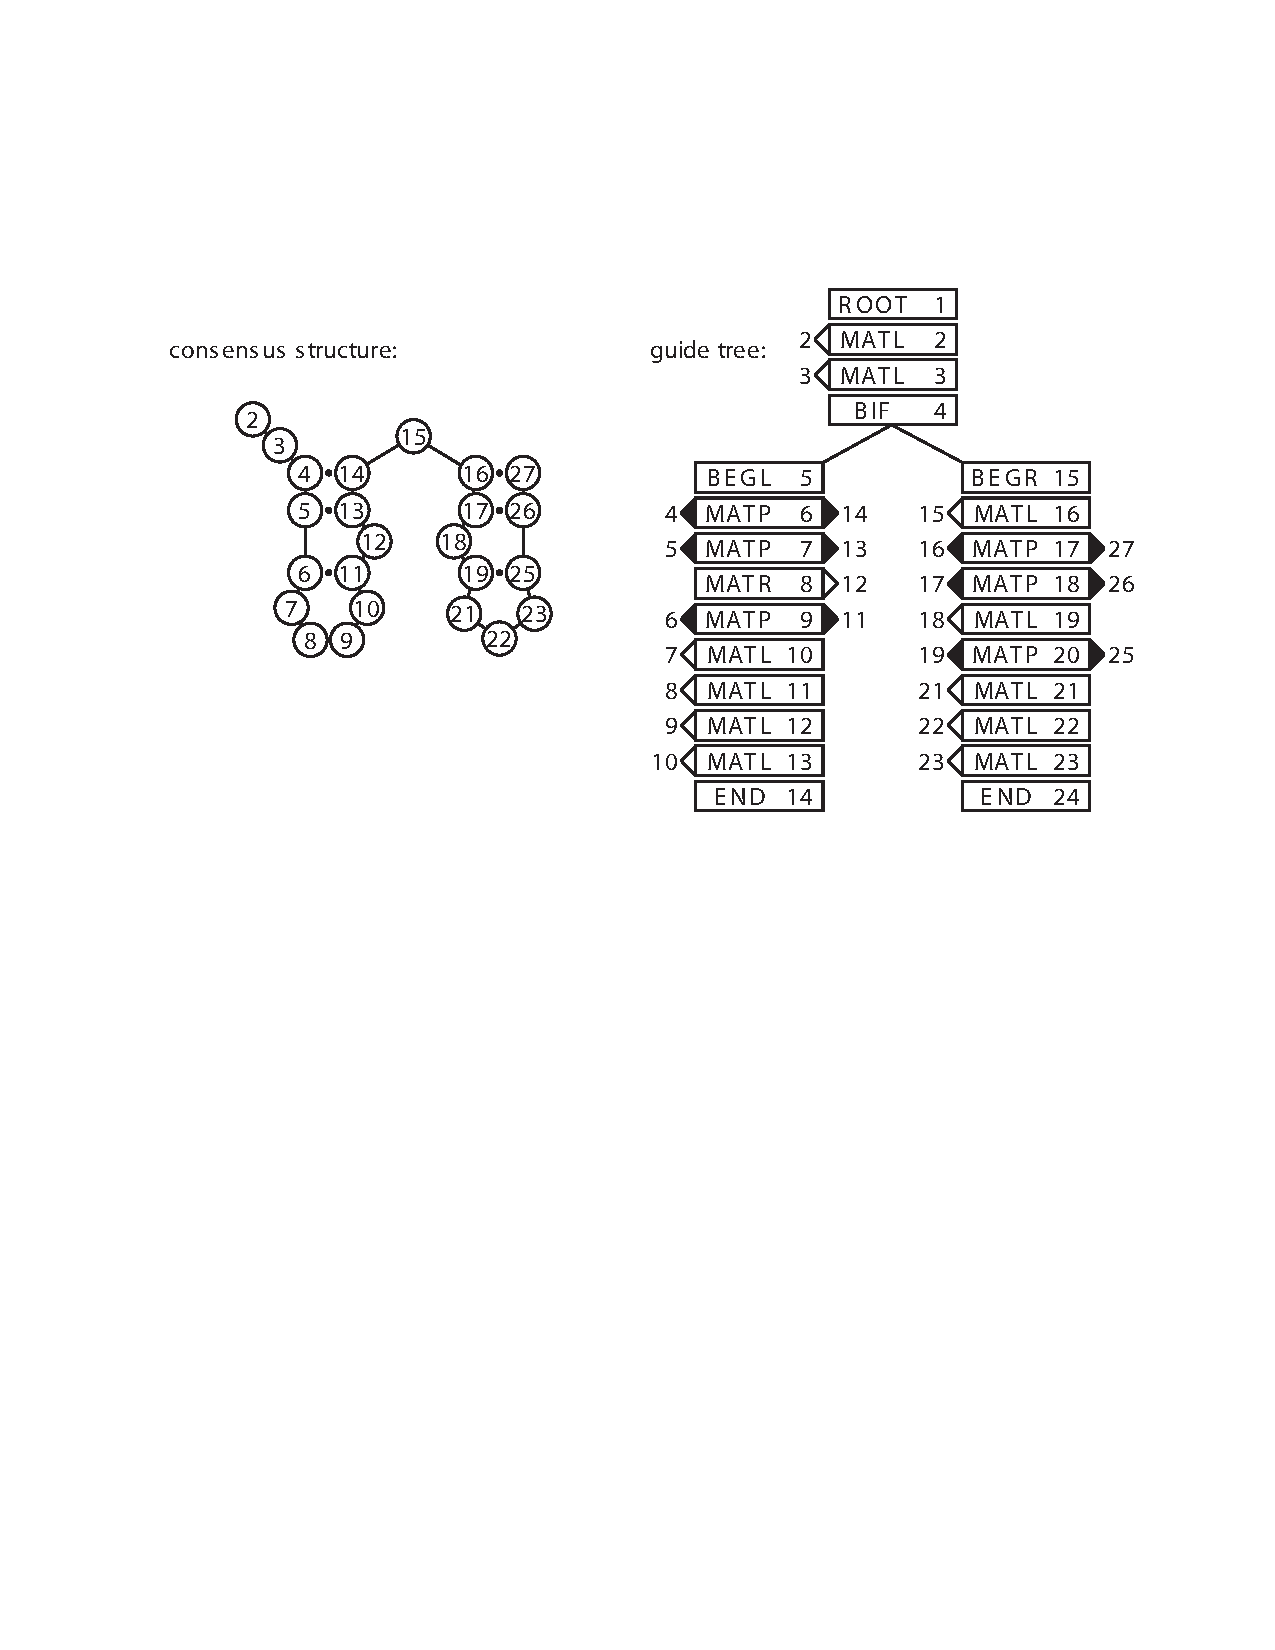
\includegraphics[width=5in]{Figures/cm_nodetree}
\end{center}
\caption{\small\textbf{The structural alignment is converted to a guide
tree.} Left: the consensus secondary structure is derived from the
annotated alignment in Figure~\ref{fig:input_alignment}. Numbers in
the circles indicate alignment column coordinates: e.g.  column 4 base
pairs with column 14, and so on. Right: the CM guide tree
corresponding to this consensus structure. The nodes of the tree are
numbered 1..24 in preorder traversal (see text). MATP, MATL, and MATR
nodes are associated with the columns they generate: e.g., node 6 is a
MATP (pair) node that is associated with the base-paired columns 4 and
14.}
\label{fig:cm_nodetree}
\end{figure}

Given the consensus structure, consensus base pairs are assigned to
MATP nodes and consensus unpaired columns are assigned to MATL or MATR
nodes. One ROOT node is used at the head of the tree.  Multifurcation
loops and/or multiple stems are dealt with by assigning one or more
BIF nodes that branch to subtrees starting with BEGL or BEGR head
nodes. (ROOT, BEGL, and BEGR start nodes are labeled differently
because they will be expanded to different groups of states; this has
to do with avoiding ambiguous parse trees for individual sequences, as
described below.) Alignment columns that are considered to be
insertions relative to the consensus structure are ignored at this
stage.

In general there will be more than one possible guide tree for any
given consensus structure. Almost all of this ambiguity is eliminated
by three conventions: (1) MATL nodes are always used instead of MATR
nodes where possible, for instance in hairpin loops; (2) in describing
interior loops, MATL nodes are used before MATR nodes; and (3) BIF
nodes are only invoked where necessary to explain branching secondary
structure stems (as opposed to unnecessarily bifurcating in single
stranded sequence). One source of ambiguity remains. In invoking a
bifurcation to explain alignment columns $i..j$ by two substructures
on columns $i..k$ and $k+1..j$, there will be more than one possible
choice of $k$ if $i..j$ is a multifurcation loop containing three or
more stems. The choice of $k$ impacts the performance of the divide
and conquer algorithm; for optimal time performance, we will want
bifurcations to split into roughly equal sized alignment problems, so
I choose the $k$ that makes $i..k$ and $k+1..j$ as close to the same
length as possible.

The result of this procedure is the guide tree. The nodes of the guide
tree are numbered in preorder traversal (e.g. a recursion of ``number
the current node, visit its left child, visit its right child'': thus
parent nodes always have lower indices than their children). The guide
tree corresponding to the input multiple alignment in
Figure~\ref{fig:input_alignment} is shown in
Figure~\ref{fig:cm_nodetree}.

\subsubsection{From guide tree to covariance model}

A CM must deal with insertions and deletions in individual sequences
relative to the consensus structure. For example, for a consensus base
pair, either partner may be deleted leaving a single unpaired residue,
or the pair may be entirely deleted; additionally, there may be
inserted nonconsensus residues between this pair and the next pair in
the stem. Accordingly, each node in the master tree is expanded into
one or more \emph{states} in the CM as follows:

\vspace{0.5em}
\begin{center}
\begin{tabular}{llccc}
       &                     & total \#& \# of split& \# of insert\\
Node   &  States             & states  & states     & states \\ \hline
MATP   & [MP ML MR D] IL IR  &   6     &   4        &  2   \\
MATL   & [ML D] IL           &   3     &   2    &  1   \\
MATR   & [MR D] IR           &   3     &   2    &  1   \\
BIF    & [B]                 &   1     &   1    &  0   \\
ROOT   & [S] IL IR           &   3     &   1    &  2   \\
BEGL   & [S]                 &   1     &   1    &  0   \\
BEGR   & [S] IL              &   2     &   1    &  1   \\
END    & [E]                 &   1     &   1    &  0   \\ \hline
\end{tabular}
\end{center}
\vspace{0.5em}

Here we distinguish between consensus (``M'', for ``match'') states
and insert (``I'') states. ML and IL, for example, are both L type
states with L type productions, but they will have slightly different
properties, as described below.

The states are grouped into a \emph{split set} of 1-4 states (shown in
brackets above) and an \emph{insert set} of 0-2 insert states. The
split set includes the main consensus state, which by convention is
first. One and only one of the states in the split set must be visited
in every parse tree (and this fact will be exploited by the divide and
conquer algorithm). The insert state(s) are not obligately visited,
and they have self-transitions, so they will be visited zero or more
times in any given parse tree.

State transitions are then assigned as follows. For bifurcation nodes,
the B state makes obligate transitions to the S states of the child
BEGL and BEGR nodes. For other nodes, each state in a split set has a
possible transition to every insert state in the \emph{same} node, and
to every state in the split set of the \emph{next} node. An IL state
makes a transition to itself, to the IR state in the same node (if
present), and to every state in the split set of the next node. An IR
state makes a transition to itself and to every state in the split set
of the next node.

There is one exception to this arrangement of transitions: insert
states that are immediately before an END node are effectively
\emph{detached} from the model by making transitions into them
impossible. This inelegant solution was imposed on the CM model
building procedure to fix a design flaw that allowed an ambiguity in
the determination of a parsetree given a structure. The detachment of
these special insert states removes this ambiguity.

This arrangement of transitions guarantees that (given the guide tree)
there is unambiguously one and only one parse tree for any given
individual structure. This is important. The algorithm will find a
maximum likelihood parse tree for a given sequence, and we wish to
interpret this result as a maximum likelihood structure, so there must
be a one to one relationship between parse trees and secondary
structures \citep{Giegerich00}.

The final CM is an array of $M$ states, connected as a directed graph
by transitions $t_v(y)$ (or probability 1 transitions $v \rightarrow
(y,z)$ for bifurcations) with the states numbered such that $(y,z)
\geq v$. There are no cycles in the directed graph other than cycles
of length one (e.g. the self-transitions of the insert states). We can
think of the CM as an array of states in which all transition
dependencies run in one direction; we can do an iterative dynamic
programming calculation through the model states starting with the
last numbered end state $M$ and ending in the root state $1$.  An
example CM, corresponding to the input alignment of
Figure~\ref{fig:input_alignment}, is shown in
Figure~\ref{fig:cm_graph}.

As a convenient side effect of the construction procedure, it is
guaranteed that the transitions from any state are to a
\emph{contiguous} set of child states, so the transitions for state
$v$ may be kept as an offset and a count. For example, in
Figure~\ref{fig:cm_graph}, state 12 (an MP) connects to states 16, 17,
18, 19, 20, and 21. We can store this as an offset of 4 to the first
connected state, and a total count of 6 connected states.  We know
that the offset is the distance to the next non-split state in the
current node; we also know that the count is equal to the number of
insert states in the current node, plus the number of split set states
in the next node. These properties make establishing the connectivity
of the CM trivial. Similarly, all the parents of any given state are
also contiguously numbered, and can be determined analogously. We are
also guaranteed that the states in a split set are numbered
contiguously.  This contiguity is exploited by the divide and conquer
implementation.

\begin{figure}[tp]
\begin{center}
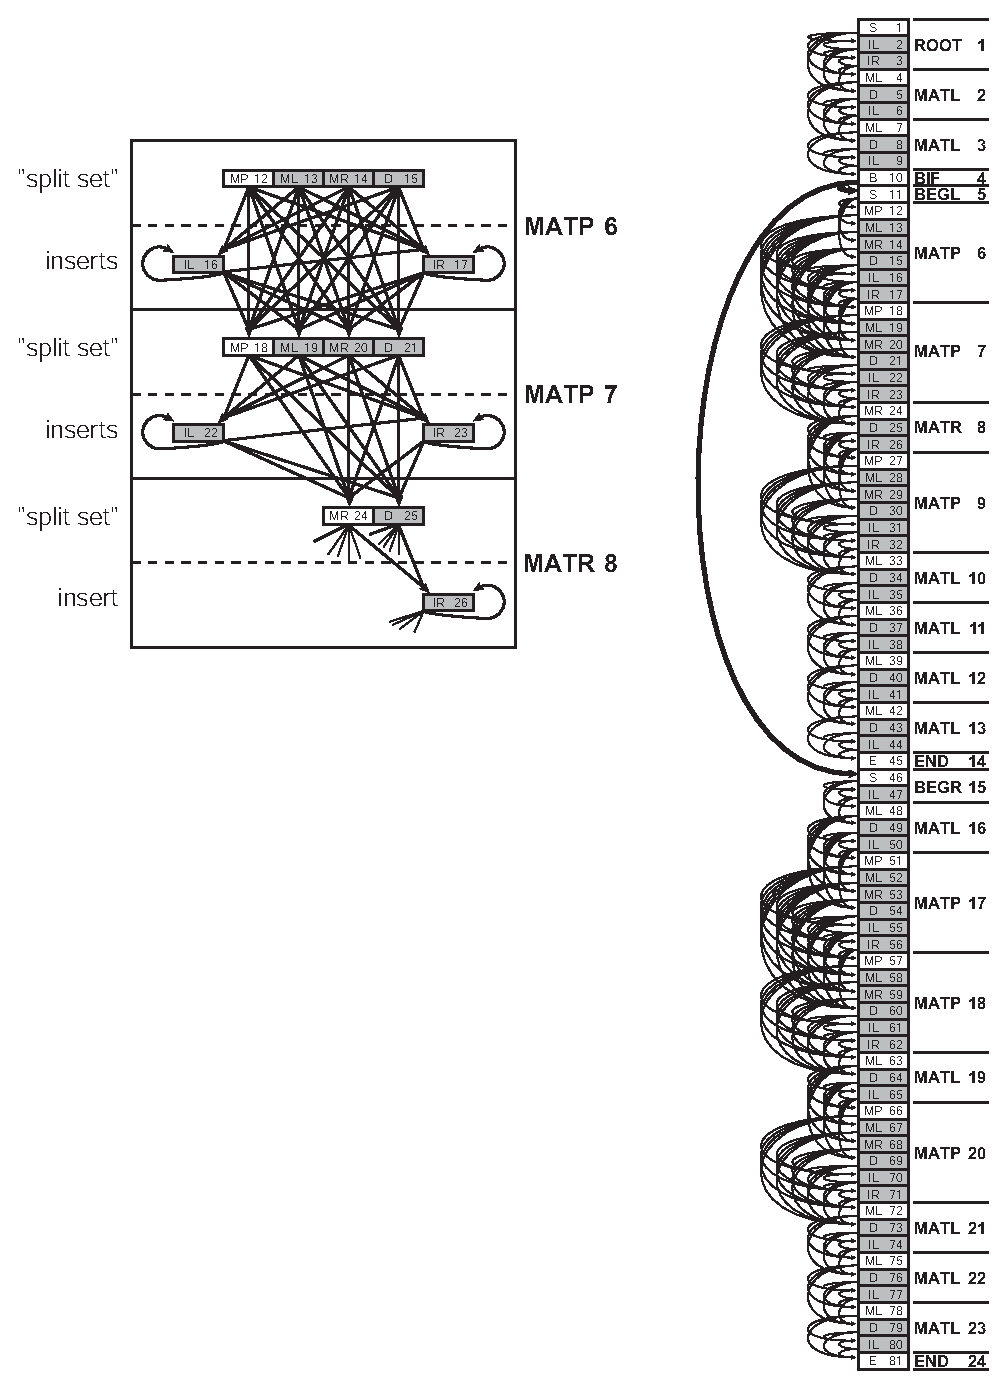
\includegraphics[width=5in]{Figures/cm_graph}
\end{center}
\caption{\small\textbf{A complete covariance model.} Right: the CM
corresponding to the alignment in Figure~\ref{fig:input_alignment}.
The model has 81 states (boxes, stacked in a vertical array). Each
state is associated with one of the 24 nodes of the guide tree (text
to the right of the state array). States corresponding to the
consensus are in white. States responsible for insertions and
deletions are gray. The transitions from bifurcation state B10 to
start states S11 and S46 are in bold because they are special: they
are an obligate (probability 1) bifurcation. All other transitions
(thin arrows) are associated with transition probabilities.  Emission
probability distributions are not represented in the figure. Left: the
states are also arranged according to the guide tree. A blow up of
part of the model corresponding to nodes 6, 7, and 8 shows
more clearly the logic of the connectivity of transition probabilities
(see main text), and also shows why any parse tree must transit through
one and only one state in each ``split set''.}
\label{fig:cm_graph}
\end{figure}

\subsubsection{Parameterization}

Using the guide tree and the final CM, each individual sequence in the
input multiple alignment can be converted unambiguously to a CM parse
tree, as shown in Figure~\ref{fig:parsetrees}. Weighted counts for
observed state transitions and singlet/pair emissions are then
collected from these parse trees. These counts are converted to
transition and emission probabilities, as maximum \emph{a posteriori}
estimates using mixture Dirichlet priors
\citep{Sjolander96,Durbin98,NawrockiEddy07}. 

\begin{figure}[t]
\begin{center}
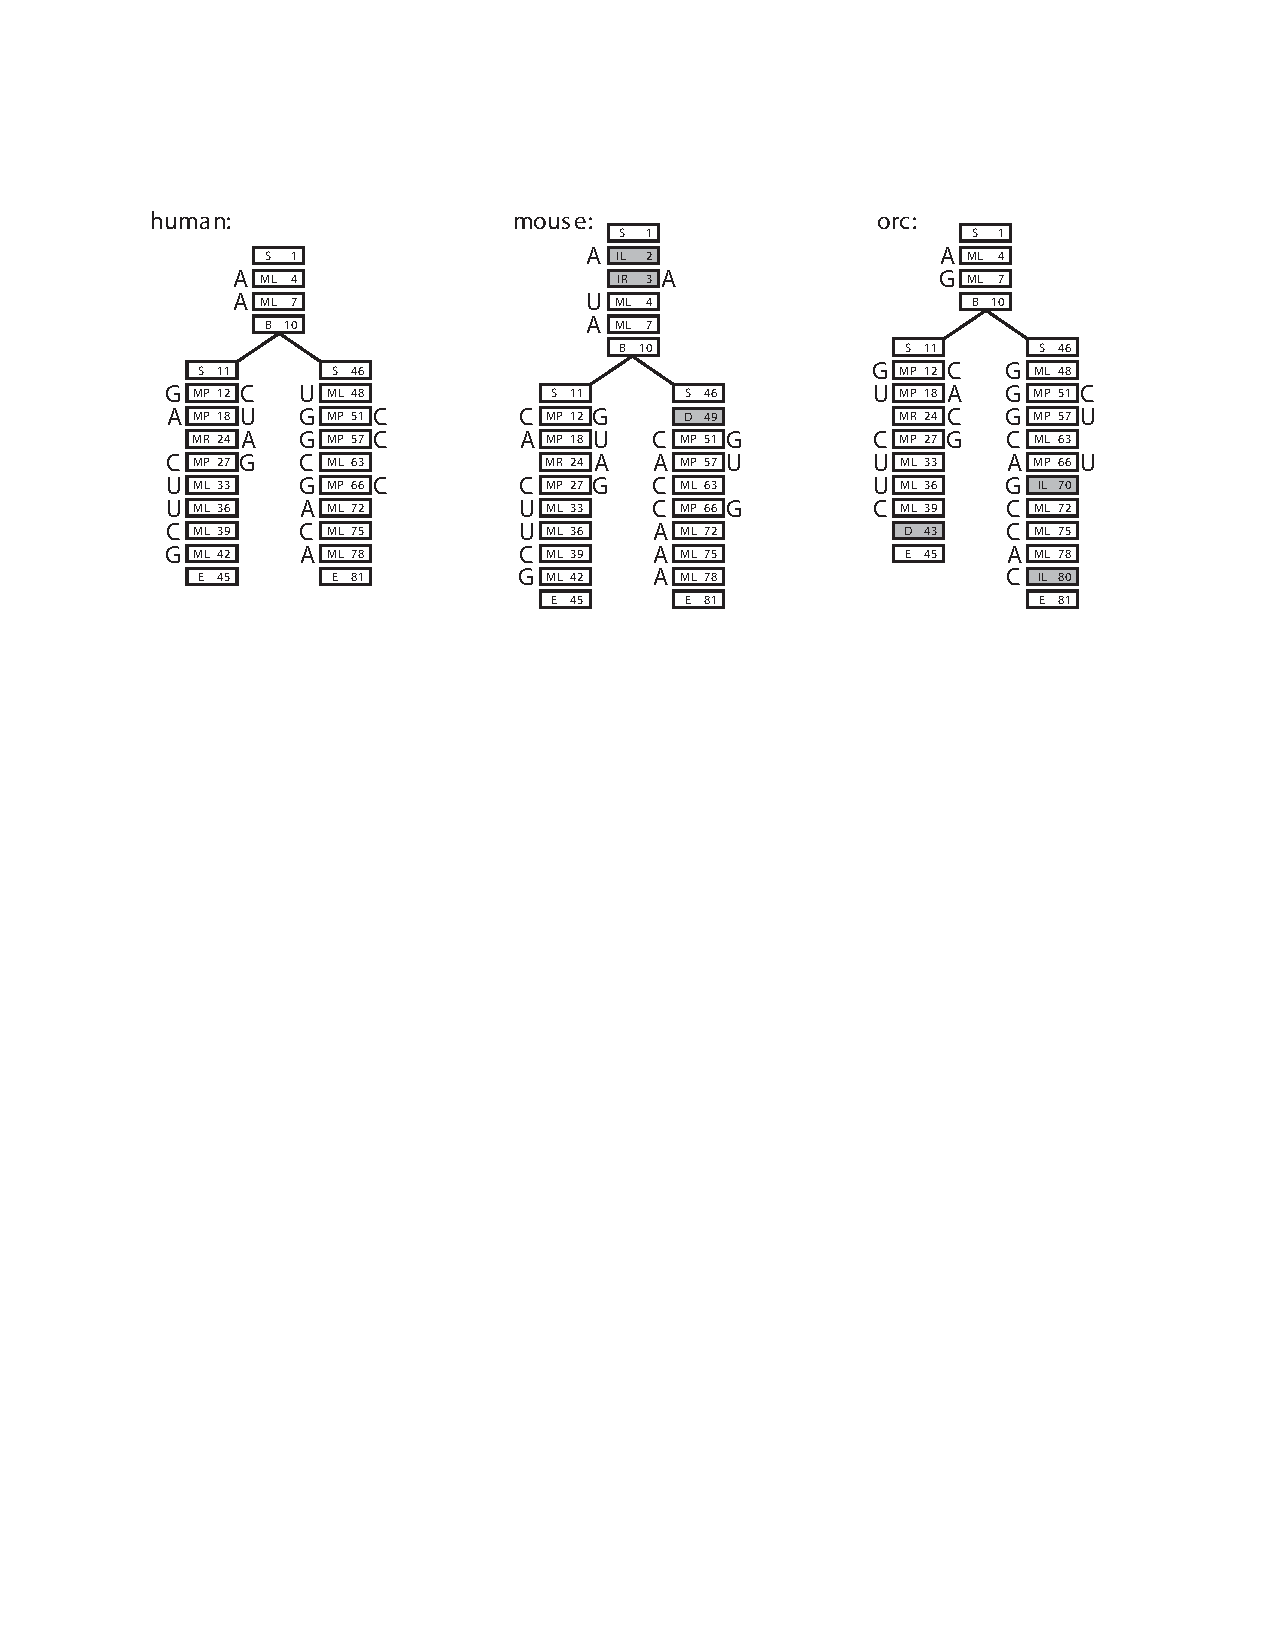
\includegraphics[width=5in]{Figures/parsetrees}
\end{center}
\caption{\small\textbf{Example parse trees.} Parse trees are shown for the
three sequences/structures from Figure~\ref{fig:input_alignment},
given the CM in Figure~\ref{fig:cm_graph}. For each sequence, each
residue must be associated with a state in the parse tree. (The
sequences can be read off its parse tree by starting at the upper left
and reading counterclockwise around the edge of parse tree.) Each
parse tree corresponds directly to a secondary structure -- base pairs
are pairs of residues aligned to MP states. A collection of parse
trees also corresponds to a multiple alignment, by aligning residues
that are associated with the same state -- for example, all three
trees have a residue aligned to state ML4, so these three residues
would be aligned together. Insertions and deletions relative to the
consensus use nonconsensus states, shown in gray.}
\label{fig:parsetrees}
\end{figure}

\subsubsection{Comparison to profile HMMs}

The relationship between an SCFG and a covariance model is analogous
to the relationship of hidden Markov models (HMMs) and profile HMMs
for modeling multiple sequence alignments
\citep{Krogh94,Durbin98,Eddy98}. A comparison may be instructive to
readers familiar with profile HMMs.  A profile HMM is a repetitive HMM
architecture that associates each consensus column of a multiple
alignment with a single type of model node -- a MATL node, in the
above notation. Each node contains a ``match'', ``delete'', and
``insert'' HMM state -- ML, IL, and D states, in the above notation.
The profile HMM also has special begin and end states. Profile HMMs
could therefore be thought of as a special case of CMs. An
unstructured RNA multiple alignment would be modeled by a guide tree
of all MATL nodes, and converted to an unbifurcated CM that would
essentially be identical to a profile HMM. (The only difference is
trivial; the CM root node includes a IR state, whereas the start node
of a profile HMM does not.) All the other node types (especially MATP,
MATR, and BIF) and state types (e.g. MP, MR, IR, and B) are SCFG
augmentations necessary to extend profile HMMs to deal with RNA
secondary structure.


\subsection{The \prog{cmbuild} program, step by step}
%\addtocontents{faq}{\textbf{Questions about using cmbuild:}}

The \prog{cmbuild} command line syntax is:

\user{cmbuild <options> [cmfile] [alifile]}

where \prog{[alifile]} is the name of the input alignment file, and
\prog{[cmfile]} is the name of the output CM file. What follows
describes the steps that \prog{cmbuild} goes through, and the most
important options that can be chosen to affect its behavior.

\subsubsection{Alignment input file}

The input alignment file must be in Stockholm format, and it must have
a consensus secondary structure annotation line (\otext{\#=GC SS\_cons}).

The program is actually capable of reading many common multiple
alignment formats (ClustalW, PHYLIP, GCG MSF, and others) but no other
format currently supports consensus RNA secondary structure
annotation. This may change in the future, either when other formats
allow structure annotation, or when \prog{cmbuild} is capable of
inferring consensus structure from the alignment by automated
comparative analysis, as the earlier COVE suite was capable
of \citep{Eddy94}. 

If the file does not exist, is not readable, or is not in a recognized
format, the program exits with a ``Alignment file doesn't exist or is
not readable'' error. If the file does not have consensus secondary
structure annotation, the program exits with a ``no consensus
structure annotation'' error. This includes all non-Stockholm
alignment files.

% EPN, Wed Apr  2 12:47:54 2008, the cat my.sto | cmbuild command
% in this faq no longer works.
\begin{srefaq}{Why does \prog{cmbuild} have a \prog{--informat} option, if it only
accepts Stockholm?} If you don't specify \prog{--informat}, the
software has to autodetect the file format. Autodetection of file
formats doesn't work in certain advanced/nonstandard cases, for
instance if you're reading the alignment from standard input instead
of from a file. The \prog{--informat} allows you to override
autodetection; e.g. \prog{cat my.sto | cmbuild --informat Stockholm
my.cm -} is an example of reading the alignment from piped standard
input.
\end{srefaq}

\subsubsection{Parsing secondary structure annotation}

The structure annotation line only needs to indicate which columns are
base paired to which. It does not have to be in full WUSS notation.
Even if it is, the details of the notation are largely ignored.
Nested pairs of \otext{<>}, \otext{()}, \otext{[]}, or \otext{{}} symbols
are interpreted as base paired columns. All other columns marked with
the symbols \otext{:,\_-.~} are interpreted as single stranded columns.

A simple minimal annotation is therefore to use \otext{<>} symbols to
mark base pairs and \otext{.} for single stranded columns.

If a secondary structure annotation line is in WUSS notation and it
contains valid pseudoknot annotation (e.g.\ additional non-nested
stems marked with AAA,aaa or BBB,bbb, etc.), this annotation is
ignored because Infernal cannot handle
pseudoknots. Internally, these columns are treated as if they were
marked with \otext{.} symbols.

\begin{srefaq}{How should I choose to annotate pseudoknots?} 
Infernal can only deal with nested base pairs. If there is
a pseudoknot, you have to make a choice of which stem to annotate as
normal nested structure (thus including it in the model) and which
stem to call additional ``pseudoknotted'' structure (thus ignoring it
in the model). For example, for a simple two-stem pseudoknot, should
you annotate it as \otext{AAAA.<<<<aaaa....>>>>}, or
\otext{<<<<.AAAA>>>>....aaaa}?  From an RNA structure viewpoint, which
stem I label as the pseudoknotted one is an arbitrary choice; but
since one of the stems in the pseudoknot will have to be modeled as a
single stranded region by Infernal, the choice makes a
slight difference in the performance of your model. You want your
model to capture as much information content as possible.  Thus, since
the information content of the model is a sum of the sequence
conservation plus the additional information contributed by pairwise
correlations in base-paired positions, you should tend to annotate the
shorter stem as the ``pseudoknot'' (modeling as many base pairs as
possible), and you should also annotate the stem with the more
conserved primary sequence as the ``pseudoknot'' (if one stem is more
conserved at the sequence level, you won't lose as much by modeling
that one as primary sequence consensus only).
\end{srefaq}

If (aside from any ignored pseudoknot annotation) the structure
annotation line contains characters other than \otext{<>()[]{}:\_-,.~}
then those characters are ignored (treated as \otext{.}) and a warning
is printed.

If, after this ``data cleaning'', the structure annotation is
inconsistent with a secondary structure (for example, if the number of
\otext{<} and \otext{>} characters isn't the same), then the program
exits with a ``failed to parse consensus structure annotation'' error.

\subsubsection{Sequence weighting}

By default, the input sequences are weighted in two ways to compensate
for biased sampling (phylogenetic correlations).  Relative sequence
weights are calculated by the Henikoff position-based method.
\citep{Henikoff94b}.  (The \prog{--wpb} option forces position-based
weights, but is redundant since that's the default.)  To turn relative
weighting off (e.g. set all weights to 1.0), use the \prog{--wnone}
option.

Some alignment file formats allow relative sequence weights to be
given in the file. This includes Stockholm format, which has
\otext{\#=GS WT} weight annotations. Normally \prog{cmbuild} ignores any
such input weights.  The \prog{--wgiven} option tells \prog{cmbuild}
to use them.  This lets you set the weights with any external
procedure you like; for example, the \prog{esl-weight} utility program in
Easel\footnote{This program will be in
  \ccode{infernal/easel/miniapps/} after building Infernal.} 
implements some common weighting algorithms,
including the Gerstein/Sonnhammer/Chothia weighting scheme
\citep{Gerstein94}.

Absolute weights (the ``effective sequence number'') is calculate by
``entropy weighting'' \citep{Karplus98}. This sets the balance between
the prior and the data, and affects the information content of the
model. Entropy weighting reduces the effective sequence number (the
total sum of the weights) and increases the entropy (degrading the
information content) of the model until a threshold is reached. The
default entropy is 1.41 bits per position (roughly 0.59 bits of
information, relative to uniform base composition). This threshold can
be changed with the \prog{--ere <x>} option. Entropy weighting may
be turned off entirely with the \prog{--enone} option.


\subsubsection{Architecture construction}

The CM architecture is now constructed from your input alignment and
your secondary structure annotation, as described in the previous
section. 

The program needs to determine which columns are consensus (match)
columns, and which are insert columns. (Remember that although WUSS
notation allows insertions to be annotated in the secondary structure
line, \prog{cmbuild} is only paying attention to annotated base
pairs.) By default, it does this by a simple rule based on the
frequency of residues (non-gaps) in a column. If the frequency of
residues is lower than a threshold, the column is considered to be
an insertion. Importantly though this frequency is determined using
the relative weights from the sequence weighting step, instead of
absolute gaps (e.g. a residue in a sequence with weight $0.8$ will count
 as $0.8$ residues).

The threshold defaults to 0.5. It can be changed to another number
\otext{<x>} (from 0 to 1.0) by the \prog{--symfrac <x>} option.  The
lower the number, the more columns are included in the model.  At
\prog{--symfrac 0.0}, all the columns are considered to be part of
the consensus. At \prog{--symfrac 1.0}, only columns with no gaps are.

You can also manually specify which columns are consensus versus
insert by including reference coordinate annotation (e.g. a
\otext{\#=GC RF} line, in Stockholm format) and using the
\prog{--hand} option. There's an example of this in the tutorial. Any
columns marked by non-gap symbols become consensus columns. (The
simplest thing to do is mark consensus columns with x's, and insert
columns with \otext{.}'s. Remember that spaces aren't allowed in
alignments in Stockholm format.) If you set the \prog{--hand} option but
your file doesn't have reference coordinate annotation, the program
exits with an error.

\subsubsection{Parameterization}

Weighted observed emission and transition counts are then collected
from the alignment data. These count vectors $c$ are then converted to
estimated probabilities $p$ using mixture Dirichlet priors
\citep{Sjolander96, Durbin98, NawrockiEddy07}. You can provide your
own prior as a file, using the \prog{--prior <f>} option.

As an exception, insert state emission probabilities are not learned
from the counts from implicit parse trees of sequences in the input
alignment, instead they are all set to 0.25 for each of the four RNA
nucleotides.  Another exception is made for transition counts in
ROOT\_IL and ROOT\_IR states from the implicit parsetrees. Any
transition counts in these states are \emph{ignored} by the
construction procedure -- they are set to zero before the transition
probability parameters for these states are determined.

\subsubsection{Naming the model}

Each CM gets a name. Stockholm format allows the alignment to have a
name, provided in the \otext{\#=GF ID} tag. If this name is provided,
it is used as the CM name.

Stockholm format allows more than one alignment per file, and
\prog{cmbuild} supports this: CM files can contain more than one
model, and if you say e.g.\ \prog{cmbuild Rfam.cm Rfam.sto} where
\otext{Rfam.sto} contains a whole database of alignments,
\prog{cmbuild} will create a database of CMs in the \prog{Rfam.cm} file,
one per alignment. 

If a name is not provided in the Stockholm \otext{\#=GF ID}
annotation, the name given to each CM is the input filename. This will
not work if the alignment file has more than one alignment. In that
case, you must include names for each alignment.

If the alignment file only has 1 alignment in it, you can override the
automatic naming conventions and provide your own name with the \prog{-n <s>}
option, where \prog{<s>} is any string. 

\subsubsection{Saving the model}

The model is now saved to a file, according to the filename specified
on the command line. By default, a new file is created, and the model
is saved in a portable ASCII text format. This format is described in
section~\ref{section:formats} of this guide.

If the cmfile already exists, the program exits with an error. The
\prog{-F} option causes the new model to overwrite an existing
cmfile. 




\newpage
\section{Tabular output formats}
\label{section:tabular}
\setcounter{footnote}{0}

\subsection{Target hits tables}

The \ccode{--tblout} output option in \prog{cmsearch} and
\prog{cmscan} produces \emph{target hits tables}. There are two
different formats of target hits table, which are both described
below. By default, both \prog{cmsearch} and \prog{cmscan} produce the
target hits table in \emph{format 1}. Format 1 is the only format that
was used by Infernal versions 1.1rc1 through 1.1.1. As of version 1.1.2,
with \prog{cmscan}, the \ccode{--fmt 2} option can be used in
combination with \ccode{--tblout} to produce a target hits table in
the alternative \emph{format 2}.  Both formats 1 and 2 target hits
table consist of one line for each different query/target comparison
that met the reporting thresholds, ranked by decreasing statistical
significance (increasing E-value).

\subsubsection{Target hits table format 1}

In the format 1 table, each line
consists of \textbf{18 space-delimited fields} followed by a free text
target sequence description, as follows:\footnote{The \ccode{tblout}
  format is deliberately space-delimited (rather than tab-delimited)
  and justified into aligned columns, so these files are suitable both
  for automated parsing and for human examination. Tab-delimited data
  files are difficult for humans to examine and spot check. For this
  reason, we think tab-delimited files are a minor evil in the
  world. Although we occasionally receive shrieks of outrage about
  this, we stubbornly feel that space-delimited files are just as
  trivial to parse as tab-delimited files.}

\begin{description}
\item[\emprog{(1) target name:}]
  The name of the target sequence or profile. 

\item[\emprog{(2) accession:}]
  The accession of the target sequence or profile, or '-' if none.

\item[\emprog{(3) query name:}] 
  The name of the query sequence or profile.

\item[\emprog{(4) accession:}]
  The accession of the query sequence or profile, or '-' if none.

\item[\emprog{(5) mdl (model):}] Which type of model was used to
  compute the final score. Either 'cm' or 'hmm'. A CM is
  used to compute the final hit scores unless the model has zero
  basepairs or the \ccode{--hmmonly} option is used, in which case a
  HMM will be used. 

\item[\emprog{(6) mdl from (model coord):}]
  The start of the alignment of this hit with respect to the
  profile (CM or HMM), numbered 1..N for a profile of N consensus positions.

\item[\emprog{(7) mdl to (model coord):}]
  The end of the alignment of this hit with respect to the
  profile (CM or HMM), numbered 1..N for a profile of N consensus positions.

\item[\emprog{(8) seq from (ali coord):}]
  The start of the alignment of this hit with respect to the
  sequence, numbered 1..L for a sequence of L residues.
 
\item[\emprog{(9) seq to (ali coord):}]
  The end of the alignment of this hit with respect to the
  sequence, numbered 1..L for a sequence of L residues.

\item[\emprog{(10) strand:}]
  The strand on which the hit occurs on the sequence. '+' if the hit is on
  the top (Watson) strand, '-' if the hit is on the bottom (Crick) strand.
  If on the top strand, the ``seq from'' value will be less than or
  equal to the ``seq to'' value, else it will be greater than or equal
  to it. 

\item[\emprog{(11) trunc:}] 
  Indicates if this is predicted to be a truncated CM hit or not. This will be
  ``no'' if it is a CM hit that is not predicted to be truncated by the end of the
  sequence, ``5'\,'' or ``3'\,'' if the hit is predicted to have one or more
  5' or 3' residues missing  due to a artificial truncation of the
  sequence, or ``5'\&3''' if the hit is predicted to have one or more
  5' residues missing and one or more 3' residues missing.
  If the hit is an HMM hit, this will always be '-'. 

\item[\emprog{(12) pass:}] 
  Indicates what ``pass'' of the pipeline the hit was detected
  on. This is probably only useful for testing and
  debugging. Non-truncated hits are found on the first pass, truncated
  hits are found on successive passes.

\item[\emprog{(13) gc:}] 
  Fraction of G and C nucleotides in the hit. 

\item[\emprog{(14) bias:}] The biased-composition correction: the bit
  score difference contributed by the null3 model for CM hits, or the
  null2 model for HMM hits. High bias scores may be a red flag for a
  false positive. It is difficult to correct for all possible ways in
  which a nonrandom but nonhomologous biological sequences can appear
  to be similar, such as short-period tandem repeats, so there are
  cases where the bias correction is not strong enough (creating false
  positives).

\item[\emprog{(15) score:}]
  The score (in bits) for this target/query comparison. It includes
  the biased-composition correction (the ``null3'' model for CM hits,
  or the ``null2'' model for HMM hits). 

\item[\emprog{(16) E-value:}] The expectation value (statistical
  significance) of the target.  This is a \emph{per query} E-value;
  i.e.\ calculated as the expected number of false positives achieving
  this comparison's score for a \emph{single} query against the search
  space $Z$. For \prog{cmsearch} $Z$ is defined as the total number of
  nucleotides in the target dataset multiplied by 2 because both strands
  are searched. For \prog{cmscan} $Z$ is the total number of
  nucleotides in the query sequence multiplied by 2 because both
  strands are searched and multiplied by the number of models in the target
  database. If you search with multiple queries and if you want to
  control the \emph{overall} false positive rate of that search rather
  than the false positive rate per query, you will want to multiply
  this per-query E-value by how many queries you're doing.

\item[\emprog{(17) inc:}] 
  Indicates whether or not this hit achieves the inclusion threshold:
  '!' if it does, '?' if it does not (and rather only achieves the
  reporting threshold). By default, the inclusion threshold is an
  E-value of 0.01 and the reporting threshold is an E-value of 10.0,
  but these can be changed with command line options as described in
  the manual pages.

\item[\emprog{(18) description of target:}] 
  The remainder of the line is the target's description line, as free text.
\end{description}

\subsubsection{Target hits table format 2}
\label{tabular-format2}

Format 2 includes all 18 of the fields from format 1 in the same order, plus 9
additional fields that are interspersed between some of the 18 from
format 1, as follows:

\begin{description}

\item[\emprog{(Before field 1 of format 1) idx:}] 
  The index of the hit in the list. The first hit has index '1', the
  second has index '2', the Nth hit has index 'N'.

\item[\emprog{(Before field 5 of format 1) clan name:}] 
  The name of the clan the model for this hit belongs to, or \ccode{-} if
  the model does not belong to a clan. A clan is a group of related
  models. For example, Rfam groups three LSU rRNA models
  (LSU\_rRNA\_archaea, LSU\_rRNA\_bacteria, and LSU\_rRNA\_eukarya)
  into the same clan. The value in this field will always be \ccode{-}
  unless the \ccode{--clanin <f>} option was used with
  \ccode{cmscan} to specify clan/model relationships in the input file
  \ccode{<f>}. See section~\ref{section:formats} for a description of
  the format of the input file used with \ccode{--clanin}.

\end{description}

The following seven fields all occur in format 2 between fields 17
('inc:') and 18 ('description of target') from format 1. 

\begin{description}

\item[\emprog{olp:}] A single character indicating the overlap status
  of this hit. Here, two hits are deemed to \emph{overlap} if they
  share at least one nucleotide on the same strand of the same
  sequence. There are three possible values in this field: \ccode{*},
  \ccode{\^} and \ccode{=}.  \ccode{*} indicates this hit does not
  overlap with any other reported hits. \ccode{\^} indicates that this
  hit does overlap with at least one other hit, but none of the hits
  that overlap with it have a higher score (occur above it in the hit
  list). \ccode{=} indicates that this hit does overlap with at least
  one other hit that has a higher score (occurs above it in the hit
  list). If the \ccode{--oclan} option was enabled, the definition of
  \emph{overlap} for the designations of the three characters
  \ccode{*}, \ccode{\^} and \ccode{=} described above changes to: two
  hits are deemed to \emph{overlap} if they share at least one
  nucleotide on the same strand of the same sequence and they are to
  models that are in the same clan. That is, only overlaps between
  hits to models that are in the same clan are counted, all other
  overlaps are ignored and not annotated.  Infernal will never report
  two overlapping hits to the same model.

\item[\emprog{anyidx:}]
For hits that have \ccode{=} in the ``olp'' field, this is the
index of the best scoring hit that overlaps with this hit.
For hits with either \ccode{*} or \ccode{\^} in the "olp" field,
this field will always be \ccode{-}.

\item[\emprog{anyfrct1:}]
For hits that have \ccode{=} in the "olp" field, this is the
fraction of the length of this hit that overlaps with the best scoring
overlapping hit (the hit index given in the "anyidx" field), to
4 significant digits. 
For hits with \ccode{-} in the "anyidx"
field, this field will always be \ccode{-}.  

\item[\emprog{anyfrct2:}]
For hits that have \ccode{=} in the "olp" field, this is the
fraction of the length of the best scoring overlapping hit (the hit
index given in the "anyidx" field) that overlaps with this hit,
to 4 significant digits. 
For hits with \ccode{-} in the "anyidx"
field, this field will always be \ccode{-}.  

\item[\emprog{winidx:}] 
For hits that have \ccode{=} in the "olp" field, this is either
\ccode{"} or the index of the best scoring hit that overlaps with this
hit that is marked as \ccode{\^} in the "olp" field. If the value
is \ccode{"} it means that the best scoring hit that overlaps with
this hit that is marked as \ccode{\^} in the "olp" field is
already listed in the "anyidx" field, which is usually the case.
For hits with either \ccode{*} or \ccode{\^} in the "olp" field,
this field will always be \ccode{-}.

\item[\emprog{winfrct1:}]
For hits that have neither \ccode{-} nor \ccode{"} in the
"winidx" field, this is the fraction of the length of this hit
that overlaps with the best scoring overlapping hit marked with
\ccode{\^} in the "olp" field (the hit index given in the
"winidx" field), to 4 significant digits.  For hits with either
\ccode{*} or \ccode{\^} in the "olp" field, this field will
always be \ccode{-}.  For hits with \ccode{-} in the "winidx"
field, this field will always be \ccode{-}.  
For hits with \ccode{"} in the "winidx"
field, this field will always be \ccode{"}.  

\item[\emprog{winfrct2:}]
For hits that have neither \ccode{-} nor \ccode{"} in the
"winidx" field, this is the
fraction of the length of the best scoring overlapping hit marked with
\ccode{\^} in the "olp" field (the hit
index given in the "winidx" field) that overlaps with this hit,
to 4 significant digits. 
  For hits with either
\ccode{*} or \ccode{\^} in the "olp" field, this field will
always be \ccode{-}.  For hits with \ccode{-} in the "winidx"
field, this field will always be \ccode{-}.  
For hits with \ccode{"} in the "winidx"
field, this field will always be \ccode{"}.  

\end{description}

The tables are columnated neatly for human readability, but do not
write parsers that rely on this columnation; rely on space-delimited
fields. The pretty columnation assumes fixed maximum widths for each
field. If a field exceeds its allotted width, it will still be fully
represented and space-delimited, but the columnation will be disrupted
on the rest of the row.

Note the use of target and query columns. A program like
\prog{cmsearch} searches a query profile against a target sequence
database. In an \prog{cmsearch} tblout file, the sequence (target)
name is first, and the profile (query) name is second. A program like
\prog{cmscan}, on the other hand, searches a query sequence against a
target profile database. In a \prog{cmscan} tblout file, the profile
name is first, and the sequence name is second. You might say, hey,
wouldn't it be more consistent to put the profile name first and the
sequence name second (or vice versa), so \prog{cmsearch} and
\prog{cmscan} tblout files were identical? Well, they
still wouldn't be identical, because the target database size used for
E-value calculations is different (total number of target nucleotides
for \prog{cmsearch}, number of target profiles times target sequence
length for \prog{cmscan}), and it's good not to forget this.

If some of the descriptions of these fields don't make sense to you,
it may help to go through the tutorial in
section~\ref{section:tutorial} and read section~\ref{section:pipeline}
of the manual. 



% Changes in options between 1.0 and 1.1 are omitted from the 1.1.2 user guide.
%\newpage
%\section{Changes in command-line options from version 1.0}
\label{section:options}
\setcounter{footnote}{0}

The following tables list options from Infernal version 1.0 programs
that have either been removed, renamed or significantly changed in
version 1.1. Many options in cmsearch and cmcalibrate have changed or
been removed, mainly because the new search pipeline (see
section~\ref{section:pipeline}) is so different from the version 1.0
pipeline. For example the version 1.0 pipeline set HMM filter
thresholds for a search in a model-dependent manner, whereas those
thresholds are model-independent in version 1.1. Also, cmalign and
cmstat in version 1.1 are significantly simpler than they were in
version 1.0 and have many fewer options. The motivation for renaming
options whose behavior did not change was for consistency with
HMMER3, so that analogous options in Infernal and HMMER have the same
name. For more information on the version 1.1 options, see the manual
pages in this guide.

\subsection{cmalign options from Infernal version 1.0.x that have changed in version 1.1.} 

\begin{tabular}{|lll|}
\hline
%\multicolumn{3}{|l|}{\prog{cmalign} options in Infernal version 1.0 that have changed in version 1.1.} \\ \hline
                       & corresponding            &                                     \\
v1.0 option            & v1.1 option              & explanation                         \\ \hline
\otext{-1}             & \otext{--outformat pfam} & renamed only; no change in behavior \\
\otext{--banddump <n>} & none                     & no longer supported \\
\otext{--beta}         & none                     & QDB alignment is no longer supported \\
\otext{--checkfb}      & none                     & no longer supported \\
\otext{--checkpost}    & none                     & no longer supported \\
\otext{--devhelp}      & none                     & no longer necessary \\
\otext{--dlev}         & none                     & no longer supported \\
\otext{--dna}          & \otext{--dnaout}         & renamed only; no change in behavior \\
\otext{--fins}         & none                     & no longer supported \\
\otext{--gapthresh}    & none                     & no longer necessary \\
\otext{--hsafe}        & none                     & no longer supported \\
\otext{--inside}       & none                     & no longer supported \\
\otext{-l}             & none                     & true by default, local alignment is now the default behavior \\
none                   & \otext{-g}               & for global alignment, use \otext{-g} \\
\otext{--merge}        & none                     & no longer supported \\
\otext{--no-null3}     & none                     & no longer supported \\
\otext{--onepost}      & none                     & no longer supported \\
\otext{-p}             & none                     & true by default \\
none                   & \otext{--noprob}         & disable posterior probability annotation with \otext{--noprob} \\
\otext{-q}             & none                     & true by default, output scores with \otext{-o} or \otext{--sfile} \\
\otext{--qdb}          & none                     & QDB alignment is no longer supported \\
\otext{--pbegin <x>}   & none                     & no longer supported; settable for a CM in \otext{cmbuild} \\
\otext{--pebegin}      & none                     & no longer supported; settable for a CM in \otext{cmbuild} \\
\otext{--pend <x>}     & none                     & no longer supported; settable for a CM in \otext{cmbuild} \\
\otext{--pfend <x>}    & none                     & no longer supported; settable for a CM in \otext{cmbuild} \\
\otext{--resonly}      & none                     & no longer supported \\
\otext{--rf}           & none                     & no longer necessary \\
\otext{--rna}          & none                     & RNA output is true by default \\
\otext{-s}             & \otext{--seed}           & renamed only; no change in behavior \\
\otext{--sums}         & none                     & no longer supported \\
\otext{--viterbi}      & none                     & no longer supported \\
\otext{--withali <f>}  & \otext{--mapali <f>}     & \otext{<f>} must now be same alignment used to build CM \\
\otext{--withpknots}   & \otext{--withstr}        & renamed only; no change in behavior \\
\hline
\end{tabular}

\subsection{cmbuild options from Infernal version 1.0.x that have changed in version 1.1.} 

\begin{tabular}{|lll|}
\hline
%\multicolumn{3}{|l|}{\prog{cmalign} options in Infernal version 1.0 that have changed in version 1.1.} \\ \hline
                       & corresponding            &                                     \\
v1.0 option            & v1.1 option              & explanation                         \\ \hline
\otext{-a}             & \otext{--indi}           & renamed only; no change in behavior \\
\otext{-A}             & none                     & no longer supported \\
\otext{--eX}           & none                     & no longer supported \\
\otext{--gapthresh <x>}& \otext{--symfrac <y>}    & renamed; IMPORTANT: use \otext{<y>} equal to \otext{1.0-<x>} \\
                       &                          & where \otext{<x>} is from \otext{--gapthresh <x>} in v1.0 \\
\otext{--ignorant}     & \otext{--noss}           & renamed             \\
\otext{--pbswitch}     & none                     & no longer supported \\
\otext{-s}             & \otext{--seed}           & renamed only; no change in behavior \\
\otext{--rf}           & \otext{--hand}           & renamed only; no change in behavior \\
\otext{--regress}      & none                     & no longer supported \\
\otext{-v}             & \otext{--verbose}        & renamed             \\
\otext{--Wbeta <f>}    & \otext{--betaW}          & renamed only; no change in behavior \\
\hline
\end{tabular}


\subsection{cmcalibrate options from Infernal version 1.0.x that have changed in version 1.1.} 

\begin{tabular}{|lll|}
\hline
%\multicolumn{3}{|l|}{\prog{cmalign} options in Infernal version 1.0 that have changed in version 1.1.} \\ \hline
                             & corresponding            &                                     \\
v1.0 option                  & v1.1 option              & explanation                         \\ \hline
\otext{--devhelp}            & none                     & no longer necessary \\
\otext{--exp-beta <x>}       & \otext{--beta <x>}       & renamed only; no change in behavior \\
\otext{--exp-cmL-glc <x>}    & \otext{-L <x>}           & renamed \\
\otext{--exp-cmL-loc <x>}    & \otext{-L <x>}           & renamed \\
\otext{--exp-ffile <f>}      & \otext{--ffile <f>}      & renamed only; no change in behavior \\
\otext{--exp-fract}          & none                     & no longer relevant; HMMs are not calibrated \\
\otext{--exp-gc <f>}         & \otext{--gc}             & renamed only; no change in behavior \\
\otext{--exp-hfile <f>}      & \otext{--hfile <f>}      & renamed only; no change in behavior \\
\otext{--exp-hmmLn-glc <x>}  & none                     & no longer necessary; HMMs are not calibrated \\
\otext{--exp-hmmLn-loc <x>}  & none                     & no longer necessary; HMMs are not calibrated \\
\otext{--exp-hmmLx <x>}      & none                     & no longer necessary; HMMs are not calibrated \\
\otext{--exp-no-qdb}         & \otext{--noqdb}          & renamed only; no change in behavior \\
\otext{--exp-pfile <f>}      & none                     & no longer supported \\
\otext{--exp-qqfile <f>}     & \otext{--qqfile <f>}     & renamed only; no change in behavior \\
\otext{--exp-random}         & \otext{--random}         & renamed only; no change in behavior \\
\otext{--exp-sfile <f>}      & \otext{--sfile <f>}      & renamed only; no change in behavior \\
\otext{--exp-tailn-cglc}     & \otext{--gtailn}         & renamed \\
\otext{--exp-tailn-cloc}     & \otext{--ltailn}         & renamed \\
\otext{--exp-tailn-hglc <x>} & none                     & no longer necessary; HMMs are not calibrated \\
\otext{--exp-tailn-hloc <x>} & none                     & no longer necessary; HMMs are not calibrated \\
\otext{--exp-tailp}          & \otext{--tailp}          & renamed \\
\otext{--exp-tailxn}         & none                     & no longer supported \\
\otext{--exp-T <x>}          & none                     & no longer supported \\
\otext{--fil-aln2bands}      & none                     & no longer necessary; HMM filter thresholds no longer used \\
\otext{--fil-dfile}          & none                     & no longer necessary; HMM filter thresholds no longer used \\
\otext{--fil-gemit}          & none                     & no longer necessary; HMM filter thresholds no longer used \\
\otext{--fil-F <x>}          & none                     & no longer necessary; HMM filter thresholds no longer used \\
\otext{--fil-N <n>}          & none                     & no longer necessary; HMM filter thresholds no longer used \\
\otext{--fil-nonbanded}      & none                     & no longer necessary; HMM filter thresholds no longer used \\
\otext{--fil-Smax-hmm <x>}   & none                     & no longer necessary; HMM filter thresholds no longer used \\
\otext{--fil-Smin-hmm <x>}   & none                     & no longer necessary; HMM filter thresholds no longer used \\
\otext{--fil-Starg-hmm <x>}  & none                     & no longer necessary; HMM filter thresholds no longer used \\
\otext{--fil-tau <x>}        & none                     & no longer necessary; HMM filter thresholds no longer used \\
\otext{--fil-Xmin-hmm <x>}   & none                     & no longer necessary; HMM filter thresholds no longer used \\
\otext{--fil-Xtarg-hmm <x>}  & none                     & no longer necessary; HMM filter thresholds no longer used \\
\otext{--forecast <n>}       & \otext{--forecast}       & no longer takes \# of processors \otext{<n>}; use in combination\\
                             &                          & with \otext{--nforecast <n>} to reproduce v1.0 behavior \\
\otext{--mxsize}             & none                     & no longer supported \\
\otext{--no-null3}           & \otext{--nonull3}        & renamed only; no change in behavior \\
\otext{--pbegin <x>}         & none                     & no longer supported; settable for a CM in \otext{cmbuild} \\
\otext{--pebegin}            & none                     & no longer supported; settable for a CM in \otext{cmbuild} \\
\otext{--pend <x>}           & none                     & no longer supported; settable for a CM in \otext{cmbuild} \\
\otext{--pfend <x>}          & none                     & no longer supported; settable for a CM in \otext{cmbuild} \\
\otext{-s}                   & \otext{--seed}           & renamed only; no change in behavior \\
\otext{-v}                   & none                     & no longer supported \\
\hline
\end{tabular}


\subsection{cmemit options from Infernal version 1.0.x that have changed in version 1.1.} 

\begin{tabular}{|lll|}
\hline
%\multicolumn{3}{|l|}{\prog{cmalign} options in Infernal version 1.0 that have changed in version 1.1.} \\ \hline
                       & corresponding            &                                     \\
v1.0 option            & v1.1 option              & explanation                         \\ \hline
\otext{-n}             & \otext{-N}               & renamed only; no change in behavior \\
\otext{-s}             & \otext{--seed}           & renamed only; no change in behavior \\
\otext{--begin <n>}    & \otext{--a5p <n>}        & renamed only; no change in behavior \\
\otext{--end <n>}      & \otext{--a3p <n>}        & renamed only; no change in behavior \\
\otext{--shmm}         & none                     & no longer supported \\
\otext{--ahmm}         & none                     & no longer supported \\
\otext{--pbegin <x>}   & none                     & no longer supported; settable for a CM in \otext{cmbuild} \\
\otext{--pebegin}      & none                     & no longer supported; settable for a CM in \otext{cmbuild} \\
\otext{--pend <x>}     & none                     & no longer supported; settable for a CM in \otext{cmbuild} \\
\otext{--pfend <x>}    & none                     & no longer supported; settable for a CM in \otext{cmbuild} \\
\hline
\end{tabular}


\subsection{cmsearch options from Infernal version 1.0.x that have changed in version 1.1.} 

\begin{tabular}{|lll|}
\hline
%\multicolumn{3}{|l|}{\prog{cmalign} options in Infernal version 1.0 that have changed in version 1.1.} \\ \hline
                           & corresponding            &                                     \\
v1.0 option                & v1.1 option              & explanation                         \\ \hline
\otext{--aln2hbands}       & none                     & no longer supported \\
\otext{--aln-hbanded}      & none                     & true by default \\
\otext{--aln-optacc}       & none                     & true by default \\
\otext{--dna}              & none                     & no longer supported \\
\otext{--fil-no-hmm}       & \otext{--nohmm}          & renamed \\
\otext{--fil-no-qdb}       & \otext{--max}            & \otext{--max} turns off all filters \\
\otext{--fil-beta <x>}     & \otext{--fbeta <x>}      & renamed \\
\otext{--fil-A-hmm <x>}    & none                     & no longer supported \\
\otext{--fil-finE-hmm <x>} & none                     & no longer supported \\
\otext{--fil-finE-qdb <x>} & none                     & no longer supported \\
\otext{--fil-finT-hmm <x>} & none                     & no longer supported \\
\otext{--fil-finT-qdb <x>} & none                     & no longer supported \\
\otext{--fil-E-hmm <x>}    & none                     & no longer supported \\
\otext{--fil-E-qdb <x>}    & none                     & no longer supported \\
\otext{--fil-S-hmm <x>}    & none                     & no longer supported \\
\otext{--fil-Smax-hmm <x>} & none                     & no longer supported \\
\otext{--fil-Smin-hmm <x>} & none                     & no longer supported \\
\otext{--fil-T-hmm <x>}    & none                     & no longer supported \\
\otext{--fil-T-qdb <x>}    & none                     & no longer supported \\
\otext{--fil-Xmin-hmm <x>} & none                     & no longer supported \\
\otext{--forecast <n>}     & none                     & no longer supported \\
\otext{--forward}          & \otext{--hmmonly}        & renamed \\
\otext{--ga}               & \otext{--cut\_ga}        & renamed only; no change in behavior \\
\otext{--gcfile <f>}       & none                     & no longer supported \\
\otext{--hbanded}          & none                     & true by default \\
\otext{--hmm-W <n>}        & none                     & no longer supported \\
\otext{--hmm-cW <x>}       & \otext{--wcx <x>}        & renamed \\
\otext{--informat <s>}     & \otext{--tformat <s>}    & renamed only; no change in behavior \\
\otext{--inside}           & none                     & true by default \\
\otext{--lambda <x>}       & none                     & no longer supported \\
\otext{--nc}               & \otext{--cut\_nc}        & renamed only; no change in behavior \\
\otext{--noalign}          & \otext{--noali}          & renamed \\
\otext{--no-qdb}           & \otext{--nonbanded}      & renamed only; no change in behavior \\
\otext{--tabfile <f>}      & \otext{--tblout <f>}     & renamed, and format of \otext{<f>} changed \\
\otext{--tc}               & \otext{--cut\_tc}        & renamed only; no change in behavior \\
\otext{--no-null3}         & \otext{--nonull3}        & renamed only; no change in behavior \\
\otext{--null2}            & none                     & no longer supported \\
\otext{-p}                 & none                     & true by default \\
\otext{--pbegin <x>}       & none                     & no longer supported; settable for a CM in \otext{cmbuild} \\
\otext{--pebegin}          & none                     & no longer supported; settable for a CM in \otext{cmbuild} \\
\otext{--pend <x>}         & none                     & no longer supported; settable for a CM in \otext{cmbuild} \\
\otext{--pfend <x>}        & none                     & no longer supported; settable for a CM in \otext{cmbuild} \\
\otext{--rna}              & none                     & true by default \\
\otext{--rtrans}           & none                     & no longer supported \\
\otext{-v}                 & none                     & no longer supported \\
\otext{--viterbi}          & none                     & no longer supported \\
\otext{-x}                 & none                     & no longer supported \\
\hline
\end{tabular}


\subsection{cmstat options from Infernal version 1.0.x that have changed in version 1.1.} 

\begin{tabular}{|lll|}
\hline
%\multicolumn{3}{|l|}{\prog{cmalign} options in Infernal version 1.0 that have changed in version 1.1.} \\ \hline
                           & corresponding            &                                     \\
v1.0 option                & v1.1 option              & explanation                         \\ \hline
\otext{-g}                 & none                     & no longer relevant\\
\otext{-m}                 & none                     & true by default \\
\otext{--le}               & none                     & no longer supported \\
\otext{--ge}               & none                     & no longer supported \\
\otext{--beta <x>}         & none                     & no longer relevant \\
\otext{--qdbfile <x>}      & none                     & no longer supported \\
\otext{--lfi}              & none                     & no longer relevant \\
\otext{--gfi}              & none                     & no longer relevant \\
\otext{--lfc}              & none                     & no longer relevant \\
\otext{--gfc}              & none                     & no longer relevant \\
\otext{-E <x>}             & none                     & \otext{-E <x>} behaves differently now \\
\otext{-T <x>}             & none                     & \otext{-T <x>} behaves differently now \\
\otext{--nc}               & none                     & no longer relevant \\
\otext{--ga}               & none                     & no longer relevant \\
\otext{--tc}               & none                     & no longer relevant \\
\otext{--seqfile <f>}      & none                     & no longer supported \\
\otext{--toponly}          & none                     & no longer supported \\
\otext{--search}           & none                     & no longer supported \\
\otext{--cmL}              & none                     & no longer supported \\
\otext{--hmmL}             & none                     & no longer supported \\
\otext{--efile <f>}        & none                     & no longer relevant \\
\otext{--bfile <f>}        & none                     & no longer relevant \\
\otext{--sfile <f>}        & none                     & no longer relevant \\
\otext{--xfile <f>}        & none                     & no longer relevant \\
\otext{--afile <f>}        & none                     & no longer relevant \\
\otext{--bits}             & none                     & no longer relevant \\
\hline
\end{tabular}


\newpage

\section{Some other topics}
\label{section:more}
\setcounter{footnote}{0}

\subsection{How do I cite HMMER?}

The appropriate citation is to the web site, \url{hmmer.org}. You
should also cite what version of the software you used. We archive all
old versions, so anyone should be able to obtain the version you used,
when exact reproducibility of an analysis is an issue. 

The version number is in the header of most output files. To see it
quickly, do something like \prog{hmmscan -h} to get a help page, and
the header will say:

\begin{sreoutput}
# hmmscan :: search sequence(s) against a profile database
# HMMER 3.1 (February 2013); http://hmmer.org/
# Copyright (C) 2011 Howard Hughes Medical Institute.
# Freely distributed under the GNU General Public License (GPLv3).
# - - - - - - - - - - - - - - - - - - - - - - - - - - - - - - - - - - - -
\end{sreoutput}

So (from the second line there) this is from HMMER 3.1.

There is not yet any appropriate citable published paper that
describes the HMMER3 software suite.



\subsection{How do I report a bug?}

Email us, at \url{hmmer@janelia.hhmi.org}.

Before we can see what needs fixing, we almost always need to
reproduce a bug on one of our machines. This means we want to have a
small, reproducible test case that shows us the failure you're seeing.
So if you're reporting a bug, please send us:

\begin{itemize}
 \item A brief description of what went wrong.
 \item The command line(s) that reproduce the problem.
 \item Copies of any files we need to run those command lines.
 \item Information about what kind of hardware you're on, what
   operating system, and (if you compiled the software yourself rather
   than running precompiled binaries), what compiler and version you
   used, with what configuration arguments.
\end{itemize}

Depending on how glaring the bug is, we may not need all this
information, but any work you can put into giving us a clean
reproducible test case doesn't hurt and often helps.

The information about hardware, operating system, and compiler is
important. Bugs are frequently specific to particular configurations
of hardware/OS/compiler.  We have a wide variety of systems available
for trying to reproduce bugs, and we'll try to match your system as
closely as we can.

If you first see a problem on some huge compute (like running a
zillion query sequence over a huge profile database), it will really,
really help us if you spend a bit of time yourself trying to isolate
whether the problem really only manifests itself on that huge compute,
or if you can isolate a smaller test case for us. The ideal bug report
(for us) gives us everything we need to reproduce your problem in one
email with at most some small attachments. 

Remember, we're not a company with dedicated support staff -- we're a
small lab of busy researchers like you. Somebody here is going to drop
what they're doing to try to help you out. Try to save us some time,
and we're more likely to stay in our usual good mood.

If we're in our usual good mood, we'll reply quickly.  We'll probably
tell you we fixed the bug in our development code, and that the fix
will appear in the next HMMER release. This of course doesn't help you
much, since nobody knows when the next HMMER release is going to be.
So if possible, we'll usually try to describe a workaround for the
bug.

If the code fix is small, we might also tell you how to patch and
recompile the code yourself. You may or may not want to do this.


There are currently not enough open bugs to justify having a formal
on-line bug tracking system. We have a bugtracking system, but it's
internal.


\subsection{Input files}

\subsubsection{Reading from a stdin pipe using - (dash) as a filename argument}

Generally, HMMER programs read their sequence and/or profile input
from files. Unix power users often find it convenient to string an
incantation of commands together with pipes (indeed, such wizardly
incantations are a point of pride). For example, you might extract a
subset of query sequences from a larger file using a one-liner
combination of scripting commands (perl, awk, whatever). To facilitate
the use of HMMER programs in such incantations, you can almost always
use an argument of '-' (dash) in place of a filename, and the program
will take its input from a standard input pipe instead of opening a
file.

For example, the following three commands are entirely equivalent, and
give essentially identical output:

\user{hmmsearch globins4.hmm uniprot\_sprot.fasta} 

\user{cat globins4.hmm | hmmsearch - uniprot\_sprot.fasta}

\user{cat uniprot\_sprot.fasta | hmmsearch globins4.hmm - }

Most Easel ``miniapp'' programs share the same ability of pipe-reading.

Because the programs for profile HMM fetching (\prog{hmmfetch}) and
sequence fetching (\prog{esl-sfetch}) can fetch any number of profiles
or sequences by names/accessions given in a list, \emph{and} these
programs can also read these lists from a stdin pipe, you can craft
incantations that generate subsets of queries or targets on the
fly. For example:

\user{esl-sfetch --index uniprot\_sprot.fasta}

\user{cat mytargs.list | esl-sfetch -f uniprot\_sprot.fasta - | hmmsearch globins4.hmm -}

This takes a list of sequence names/accessions in
\prog{mytargets.list}, fetches them one by one from UniProt (note that
we index the UniProt file first, for fast retrieval; and note that
\prog{esl-sfetch} is reading its \prog{<namefile>} list of
names/accessions through a pipe using the '-' argument), and pipes
them to an \prog{hmmsearch}. It should be obvious from this that we
can replace the \prog{cat mytargets.list} with \emph{any} incantation
that generates a list of sequence names/accessions (including SQL
database queries).

Ditto for piping subsets of profiles. Supposing you have a copy of Pfam in Pfam-A.hmm:

\user{hmmfetch --index Pfam-A.hmm}

\user{cat myqueries.list | hmmfetch -f Pfam.hmm - | hmmsearch - uniprot\_sprot.fasta}

This takes a list of query profile names/accessions in
\prog{myqueries.list}, fetches them one by one from Pfam, and does an
hmmsearch with each of them against UniProt. As above, the \prog{cat
  myqueries.list} part can be replaced by any suitable incantation
that generates a list of profile names/accessions.

There are three kinds of cases where using '-' is restricted or
doesn't work. A fairly obvious restriction is that you can only use
one '-' per command; you can't do a \prog{hmmsearch - -} that tries to
read both profile queries and sequence targets through the same stdin
pipe. Second, another case is when an input file must be obligately
associated with additional, separately generated auxiliary files, so
reading data from a single stream using '-' doesn't work because the
auxiliary files aren't present (in this case, using '-' will be
prohibited by the program). An example is \prog{hmmscan}, which needs
its \prog{<hmmfile>} argument to be associated with four auxiliary
files named \prog{<hmmfile>.h3\{mifp\}} that \prog{hmmpress} creates,
so \prog{hmmscan} does not permit a '-' for its \prog{<hmmfile>}
argument. Finally, when a command would require multiple passes over
an input file, the command will generally abort after the first pass
if you are trying to read that file through a standard input pipe
(pipes are nonrewindable in general; a few HMMER or Easel programs
will buffer input streams to make multiple passes possible, but this
is not usually the case). An example would be trying to search a file
containing multiple profile queries against a streamed target
database:

\user{cat myqueries.list | hmmfetch -f Pfam.hmm > many.hmms}

\user{cat mytargets.list | esl-sfetch -f uniprot\_sprot.fasta - | hmmsearch many.hmms -}

This will fail. Unfortunately the above business about how it will
``generally abort after the first pass'' means it fails weirdly. The
first query profile search will succeed, and its output will appear;
then an error message will be generated when \prog{hmmsearch} sees the
\emph{second} profile query and oops, it realizes it is unable to
rewind the target sequence database stream. This is inherent in how it
reads the profile HMM query file sequentially as a stream (which is
what's allowing it to read input from stdin pipes in the first place),
one model at a time: it doesn't see there's more than one query model
in the file until it gets to the second model.

This case isn't too restricting because the same end goal can be
achieved by reordering the commands. In cases where you want to do
multiple queries against multiple targets, you always want to be
reading the \emph{queries} from a stdin pipe, not the targets:

\user{cat mytargets.list | esl-sfetch -f uniprot\_sprot.fasta > mytarget.seqs}

\user{cat myqueries.list | hmmfetch -f Pfam.hmm - |  hmmsearch - mytarget.seqs}

So in this multiple queries/multiple targets case of using stdin
pipes, you just have to know, for any given program, which file it
considers to be queries and which it considers to be targets. (That
is, the logic in searching many queries against many targets is ``For
each query: search the target database; then rewind the target
database to the beginning.'') For \prog{hmmsearch}, the profiles are
queries and sequences are targets. For \prog{hmmscan}, the reverse.

In general, HMMER and Easel programs document in their man page
whether (and which) command line arguments can be replaced by '-'.
You can always check by trial and error, too. The worst that can
happen is a ``Failed to open file -'' error message, if the program
can't read from pipes.




\newpage
\input{manpages}

\newpage
\section{File and output formats}
\label{section:formats}
\setcounter{footnote}{0}

\subsection{Infernal CM files}

The file \prog{tutorial/Cobalamin.c.cm} gives an example of an Infernal ASCII
CM save file. An abridged version is shown here, where (\ldots) mark
deletions made for clarity and space:

\begin{tinysreoutput}
INFERNAL1/a [1.1 | June 2012]
NAME     Cobalamin
ACC      RF00174
DESC     Cobalamin riboswitch
STATES   592
NODES    163
CLEN     191
W        460
ALPH     RNA
RF       no
CONS     yes
MAP      yes
DATE     Wed Jun 13 05:40:07 2012
COM      [1] ./cmbuild Cobalamin.cm ../tutorial/Cobalamin.sto
COM      [2] ./cmcalibrate Cobalamin.cm
PBEGIN   0.05
PEND     0.05
WBETA    1e-07
QDBBETA1 1e-07
QDBBETA2 1e-15
N2OMEGA  1.52588e-05
N3OMEGA  1.52588e-05
ELSELF   -0.08926734
NSEQ     431
EFFN     6.652168
CKSUM    2307274568
NULL     0.000  0.000  0.000  0.000 
GA       39.00
TC       39.00
NC       38.79
EFP7GF   -9.3826 0.71319
ECMLC    0.69050    -9.55632    -0.82028     1600000      499982  0.002400
ECMGC    0.33713   -30.56949   -21.45119     1600000        8652  0.046232
ECMLI    0.68481    -7.98572     0.30786     1600000      351369  0.003415
ECMGI    0.38286   -21.23885   -13.16656     1600000        8796  0.045475
CM
                                             [ ROOT    0 ]      -      - - - - -
     S     0    -1 0     1     4     0     1   460   771  -8.175  -8.382  -0.025  -6.528                 
    IL     1     1 2     1     4    86   133   462   774  -1.686  -2.369  -1.117  -4.855                  0.000  0.000  0.000  0.000 
    IR     2     2 3     2     3    86   133   462   774  -1.442  -0.798  -4.142                          0.000  0.000  0.000  0.000 
                                             [ MATL    1 ]      1      - u - - -
    ML     3     2 3     5     3    86   132   461   772  -9.129  -0.009  -7.783                          0.192 -0.324 -0.320  0.331 
     D     4     2 3     5     3    80   128   458   769  -6.226  -1.577  -0.618                         
    IL     5     5 3     5     3    85   132   461   773  -1.442  -0.798  -4.142                          0.000  0.000  0.000  0.000 
(...)
                                             [ MATL   98 ]    151      - C - - -
    ML   588   587 3   590     2     1     1     1     1       *   0.000                                 -3.022  1.825 -3.061 -2.226 
     D   589   587 3   590     2     0     0     0     0       *   0.000                                 
    IL   590   590 3   590     2     1     1    13    28  -1.823  -0.479                                  0.000  0.000  0.000  0.000 
                                             [ END    99 ]      -      - - - - -
     E   591   590 3    -1     0     0     0     0     0                                                 
//
HMMER3/f [i1.1 | June 2012]
NAME  Cobalamin
ACC   RF00174
DESC  Cobalamin riboswitch
LENG  191
MAXL  565
ALPH  RNA
RF    no
MM    no
CONS  yes
CS    yes
MAP   yes
DATE  Wed Jun 13 05:40:08 2012
COM   [1] ./cmbuild Cobalamin.cm ../tutorial/Cobalamin.sto
NSEQ  431
EFFN  4.955421
CKSUM 2307274568
STATS LOCAL MSV      -10.2356  0.71319
STATS LOCAL VITERBI  -12.2484  0.71319
STATS LOCAL FORWARD   -3.9056  0.71319
HMM          A        C        G        U   
            m->m     m->i     m->d     i->m     i->i     d->m     d->d
  COMPO   1.37169  1.39466  1.27962  1.51293
          1.38629  1.38629  1.38629  1.38629
          0.02747  4.30141  4.30141  1.46634  0.26236  0.00000        *
      1   1.24903  1.60847  1.61442  1.15831      1 u - - :
          1.38629  1.38629  1.38629  1.38629
          0.02747  4.30141  4.30141  1.46634  0.26236  1.09861  0.40547
(...)
    191   1.51542  1.17791  1.56046  1.33817    441 c - - :
          1.38629  1.38629  1.38629  1.38629
          0.01381  4.28939        *  1.46634  0.26236  0.00000        *
//
\end{tinysreoutput}

A CM file consists of one or more CMs and associated filter
HMMs. Each CM is immediately followed by its filter HMM, this is
mandatory. Each CM starts with a format version identifier (here,
\prog{INFERNAL1/a}) and ends with \prog{//} on a line by itself. Each
HMM also starts with a format version identifier (here,
\prog{HMMER3/f}) and ends with \prog{//} on a line by itself.  The
format version identifier allows backward compatibility as the
Infernal software evolves: it tells the parser this file is from
Infernal's save file format version a. The closing \prog{//} allows
Infernal to determine when a CM ends and its profile HMM begins, and
allows multiple CM/filter HMM pairs to be concatenated together into a
single file.

The CM format is divided into two regions. The first region contains
textual information and miscalleneous parameters in a roughly
tag-value scheme. This section ends with a line beginning with the
keyword \prog{CM}. The second region is a tabular, whitespace-limited
format for the main model parameters.

All emission and transition model parameters are stored as log-odds
scores in bits with three digits of precision to the right of the
decimal point, rounded. 
%For example, a probability of $0.25$ is stored
%as $\log_2 0.25 = -1.38629$. 
The special case of a score of infinity, corresponding to an
impossible emission or transition, is stored as '*'.

Spacing is arranged for human readability, but the parser only cares
that fields are separated by at least one space character.

The CM format is described in more detail below, followed by a
description of the HMMER3 HMM format for the CM's mandatory filter HMM
filter.

\subsubsection{CM header section}

The header section is parsed line by line in a tag/value format. Each
line type is either \textbf{mandatory} or \textbf{optional} as
indicated. 

\begin{sreitems}{QDBBETA1 <f>}

\item [\emprog{INFERNAL1/a}] Unique identifier for the save file format
  version; the \prog{/a} means that this is INFERNAL1 CM file format
  version a. When INFERNAL changes its save file format, the revision
  code advances. This way, parsers may easily remain backwards
  compatible. The remainder of the line after the \prog{INFERNAL1/a} tag
  is free text that is ignored by the parser. INFERNAL currently writes
  its version number and release date in brackets here,
  e.g. \prog{[1.1 | June 2012]} in this
  example. \textbf{Mandatory.}

\item [\emprog{NAME <s>}] Model name; \prog{<s>} is a single word
containing no spaces or tabs. The name is normally picked up from the
\verb+#=GF ID+ line from a Stockholm alignment file.  If this is not
present, the name is created from the name of the alignment file by
removing any file type suffix. For example, an otherwise nameless CM
built from the alignment file \prog{tRNA.sto} would be named
\prog{tRNA}.  \textbf{Mandatory.}

\item [\emprog{ACC <s>}] Accession number; \prog{<s>} is a one-word
accession number. This is picked up from the \verb+#=GF AC+ line in a
Stockholm format alignment. \textbf{Optional.}

\item [\emprog{DESC <s>}] Description line; \prog{<s>} is a one-line
free text description. This is picked up from the \verb+#=GF DE+ line
in a Stockholm alignment file. \textbf{Optional.}

\item [\emprog{STATES <d>}] Number of states; \prog{<d>}, a positive nonzero
integer, is the number of states in the model.
\textbf{Mandatory.}

\item [\emprog{CLEN <d>}] Consensus model length; \prog{<d>}, a positive nonzero
integer, is the number of consensus positions in the model, which
equals the number of MATL nodes plus the number of MATR nodes plus two
times the number of MATP nodes.
\textbf{Mandatory.}

\item [\emprog{W <d>}] Window length; \prog{<d>}, a positive nonzero
integer, is the length in residues of the maximum expected size of a
hit to this model. This is calculated based on the transition
probabilities of the model\footnote{Specifically, \prog{W} is set as
the \emph{dmax} value for the ROOT\_S state (state 0) from the QDB
algorithm using $\beta$ equal to the \prog{WBETA} value
\citep{NawrockiEddy07}.}  \textbf{Mandatory.}

\item [\emprog{ALPH <s>}] Symbol alphabet type. Currently this will
necessarily be \prog{RNA} for RNA sequence analysis models.
The symbol alphabet size $K$ is set to 4 and the 
symbol alphabet to ``ACGU''. \textbf{Mandatory.}

\item [\emprog{RF <s>}] Reference annotation flag; \prog{<s>} is
either \prog{no} or \prog{yes} (case insensitive). If \prog{yes}, the
reference annotation character field(s) for each match state in the
main model (see below) is valid; if \prog{no}, these characters are
ignored.  Reference column annotation is picked up from a Stockholm
alignment file's \verb+#=GC RF+ line. by \prog{cmbuild}. It is
propagated to alignment outputs, and also may optionally be used to
define consensus match columns in CM 
construction. \textbf{Optional}; assumed to be no if not present.

\item [\emprog{CONS <s>}] Consensus residue annotation flag;
  \prog{<s>} is either \prog{no} or \prog{yes} (case insensitive).  If
  \prog{yes}, the consensus residue field(s) for each match state in
  the main model (see below) is valid. If \prog{no}, these characters
  are ignored. Consensus residue annotation is determined when models
  are built. For models of single sequences, the consensus is the same
  as the query sequence. For models of multiple alignments, the
  consensus is the highest scoring residue or basepair for each match
  state. Upper case MATL\_ML and MATR\_MR (single stranded) residues
  indicate that the model emission's score for the consensus residue
  is $\geq$ to 1.0 bit. Upper case MATP\_MP basepairs indicate that
  the model emission's score for the consensus basepair is $\geq$ to
  3.0 bits.

\item [\emprog{MAP <s>}] Map annotation flag; \prog{<s>} is either
\prog{no} or \prog{yes} (case insensitive).  If set to \prog{yes}, the
map annotation field in the main model (see below) is valid; if
\prog{no}, that field will be ignored.  The CM/alignment map
annotates each match state with the index of the alignment column from
which it came. It can be used for quickly mapping any subsequent
CM alignment back to the original multiple alignment, via the model.
\textbf{Optional}; assumed to be no if not present.

\item [\emprog{DATE <s>}] Date the model was constructed; \prog{<s>}
is a free text date string.  This field is only used for logging
purposes.\footnote{Infernal does not use dates for any purpose other than
human-readable annotation, so it is no more prone than you are to Y2K,
Y2038, or any other date-related eschatology.} \textbf{Optional.}

\item [\emprog{COM [<n>] <s>}] Command line log; \prog{<n>} counts
command line numbers, and \prog{<s>} is a one-line command. There may
be more than one \prog{COM} line per save file, each numbered starting
from $n=1$. These lines record every Infernal command that modified the
save file. This helps us reproducibly and automatically log how Rfam
models have been constructed, for example. \textbf{Optional.}

\item [\emprog{PBEGIN <f>}] Local begin probability; The aggregate
probability of a local begin into any internal entry state is
\prog{<f>}. The probability of a local begin into any single internal
entry state is \prog{<f>} divided by the number of internal entry
states in the model. All MATP\_MP, MATL\_ML, MATR\_MR, and BIF\_B
states, except for any in the the second node of the model (first
non-ROOT node), are internal entry states. The local begin probability
does not affect any of the emission/transition parameters in the CM
file, which correspond to the CM in \emph{global} search/alignment
mode, but it does affect the calibration of E-value parameters for
local search by \prog{cmcalibrate}. \prog{cmsearch} and \prog{cmscan}
therefore need to read this probability from the CM file in order to
use the same local begin probabilities used during calibration and
report appropriate E-values. \textbf{Optional}; assumed to be $0.05$
if not present.

\item [\emprog{PEND <f>}] Local end probability; The aggregate
probability of a local end out of any internal exit state is
\prog{<f>}. The probability of a local end out of any single internal
entry state is \prog{<f>} divided by the number of internal exit
states in the model. All MATP\_MP, MATL\_ML, MATR\_MR, BEGL\_S, and
BEGR\_S states, except for any for which the following node is an END
node, are internal exit states. The local end probability
does not affect any of the emission/transition parameters in the CM
file, which correspond to the CM in \emph{global} search/alignment
mode, but it does affect the calibration of E-value parameters for
local search by \prog{cmcalibrate}. \prog{cmsearch} and \prog{cmscan}
therefore need to read this probability from the CM file in order to
use the same local end probabilities used during calibration and
report appropriate E-values. \textbf{Optional}; assumed to be $0.05$
if not present.

\item [\emprog{WBETA <f>}] Tail loss probability for calculating
  window length (W); The QDB algorithm \citep{NawrockiEddy07} was used
  to determine the maximum expected length of a hit (W) using a tail
  loss probability of \otext{<f>}, W was set as the \emph{dmax} value for the
  ROOT\_S state (state 0). \textbf{Mandatory.}

\item [\emprog{QDBBETA1 <f>}] Tail loss probability for calculating
  the tighter of the two sets of query-dependent bands (QDBs); The QDB
  algorithm \citep{NawrockiEddy07} was used to determine the minimum
  and maximum subsequence lengths allowed to align to the subtree
  rooted at each state of the model, using a tail loss $\beta$
  probability of \otext{<f>}. These minimum and maximum values for each state
  are included in each state line in the main model section, described
  below.  below. The \prog{<f>} value for \prog{QDBBETA2} will be
  less than or equal to the \prog{<f>} value for \prog{QDBBETA1}.
  \textbf{Mandatory.}

\item [\emprog{QDBBETA2 <f>}] Tail loss probability for calculating
  the looser of the two sets of query-dependent bands (QDBs); The QDB
  algorithm \citep{NawrockiEddy07} was used to determine the minimum
  and maximum subsequence lengths allowed to align to the subtree
  rooted at each state of the model, using a tail loss $\beta$
  probability of \prog{<f>}. These minimum and maximum values for each state
  are included in each state line in the main model section, described
  below. The \prog{<f>} value for \prog{QDBBETA2} will be less than
  or equal to the \prog{<f>} value for \prog{QDBBETA1}.
  \textbf{Mandatory.}

\item [\emprog{N2OMEGA <f>}] The prior probability for the alternative
  ``null2'' model for biased composition
  sequences. \textbf{Mandatory}; but only relevant in \prog{cmsearch} and
  \prog{cmscan} if the \prog{--null2} option is used.

\item [\emprog{N3OMEGA <f>}] The prior probability for the alternative
  ``null3'' model for biased composition
  sequences. \textbf{Mandatory}; the null3 model is used by default in 
  \prog{cmcalibrate}, \prog{cmsearch} and \prog{cmscan}.

\item [\emprog{NSEQ <d>}] Sequence number; \prog{<d>} is a nonzero
positive integer, the number of sequences that the CM was trained on,
i.e. the number of sequences in the input alignment used to create the
CM in \prog{cmbuild}.  This field is only used for logging
purposes.  \textbf{Optional.}

\item [\emprog{EFFN <f>}] Effective sequence number; \prog{<f>} is a
nonzero positive real, the effective total number of sequences
determined by \prog{cmbuild} during sequence weighting, for combining
observed counts with Dirichlet prior information in parameterizing the
model. This field is only used for logging purposes.
\textbf{Optional.}

\item [\emprog{CKSUM <d>}] Training alignment checksum; \prog{<d>} is
  a nonnegative unsigned 32-bit integer. This number is calculated
  from the training sequence data, and used in conjunction with the
  alignment map information to verify that a given alignment is indeed
  the alignment that the map is for. \textbf{Optional.}

\item [\emprog{NULL <f> <f> <f> <f>}] null model emission scores for
  each alphabet symbol. By default, these are all \prog{0.0} but may
  not be if the \prog{--null} option was used in \prog{cmbuild} to
  define alternative null model scores. Because only RNA CMs can be
  built by \prog{cmbuild} there will be four values on this line, one
  each for ``A'', ``C'', ``G'', and ``U''. \textbf{Mandatory.}

\item [\emprog{GA <f>}] Rfam GA gathering threshold bit score.  The GA
bit score threshold is normally picked up from the \verb+#=GF GA+ line
from a Stockholm alignment file.  GA thresholds are generally
considered to be the reliable curated thresholds defining family
membership; for example, in Rfam, these thresholds define what gets
included in Rfam Full alignments based on searches with Rfam Seed
models. \textbf{Optional.}

\item [\emprog{NC <f>}] Rfam NC noise cutoff bit score.
The NC bit score threshold is normally picked up from the
\verb+#=GF NC+ line from a Stockholm alignment file.  
NC thresholds are generally considered to be the
score of the highest-scoring known false positive found by searches
during preparation of the Rfam database. \textbf{Optional.}

\item [\emprog{TC <f>}] Rfam TC trusted cutoff bit score.
The TC bit score threshold is normally picked up from the
\verb+#=GF TC+ line from a Stockholm alignment file.  
TC thresholds are generally considered to be the score of the lowest
scoring believed true positive that is above all known false positives
found by searches during preparation of the Rfam database.
\textbf{Optional.}

\item [\emprog{EFP7GF <f1> <f2>}] Statistical parameters for filter HMM
  E-value calculations in glocal mode for the Forward algorithm. 
  \prog{<f1>} and \prog{<f2>} are $\tau$ and $\lambda$ for exponential
  tails for glocal Forward filter HMM scores. This line is necessary
  in the CM file section rather than the filter HMM file because
  glocal HMM searches are not normally performed in HMMER3, but are
  part of the HMM filter pipeline in Infernal. \textbf{Mandatory.}

\item [\emprog{ECMLC <f1> <f2> <f3> <d1> <d2> <f4>}] Statistical
  parameters needed for E-value calculations for the CM CYK algorithm
  in local mode. This line, along with the next three, with tags
  \prog{ECMGC}, \prog{ECMLI}, and \prog{ECMGI}, must either all be
  present or none of them must be present. If present, the model is
  considered calibrated for E-value statistics. These lines will not
  be present in a model after it is created by \prog{cmbuild} but will
  be added by the \prog{cmcalibrate} program.  \prog{<f1>} and
  \prog{<f2>} are $\lambda$ and $\tau$, the slope and location
  parameters for exponential tails for local CYK scores. $\lambda$
  values must be positive. The remaining values were computed in
  \prog{cmcalibrate} during model calibration: \prog{<f3>} is a
  different $\tau$ value computed for the full histogram of all hits;
  \prog{<d1>} is the database size in residues; \prog{<d2>} is the
  total number of non-overlapping hits of any score found; \prog{<f4>}
  is the fraction of the high-scoring histogram tail fit to an
  exponential tail. Of these parameters, only \prog{<f1>}, \prog{<f2>}
  and \prog{<d2>} are used, the others are only stored in the CM file
  for record keeping purposes.

\item [\emprog{ECMGC <f1> <f2> <f3> <d1> <d2> <f4>}] Statistical
  parameters analogous to those described above in the \prog{ECMLC}
  line, except that these pertain to CM CYK scores in glocal mode.

\item [\emprog{ECMLI <f1> <f2> <f3> <d1> <d2> <f4>}] Statistical
  parameters analogous to those described above in the \prog{ECMLC}
  line, except that these pertain to CM Inside scores in local mode.

\item [\emprog{ECMGI <f1> <f2> <f3> <d1> <d2> <f4>}] Statistical
  parameters analogous to those described above in the \prog{ECMLC}
  line, except that these pertain to CM Inside scores in glocal mode.

\item [\emprog{CM}] Flags the start of the main model
section. \textbf{Mandatory.}

\end{sreitems}

\subsubsection{CM main model section}

All the remaining fields are \textbf{mandatory}.

The model section consistes of two types of lines: node lines and
state lines. Each node line is immediately followed by one or more
state lines, one each for each state within the node. 

\begin{sreitems}{\textbf{State line}}

\item [\textbf{Node line}] Each node line begins with 45 spaces, and
  includes ten fields. 

  The first field is always a \prog{[} character.

  The second is the node type, one of ROOT, MATP, MATL, MATR, BIF,
  BEGL, BEGR, or END. 

  The next field is the index of the node in the
  model, greater than or equal to 0. Node indices are not always in
  increasing order, e.g. node 200 may come on a line before node 100.

  The fourth field is always a \prog{]} character. 

  The next two fields are the \prog{MAP} annotation for this node. If
  \prog{MAP} was \prog{yes} in the header and the node is a MATP
  (match pair) node, then these fields will both be positive integers,
  representing the alignment column indices for the left and right
  halves of this match pair state, respectively. If \prog{MAP} was
  \prog{yes} and the node is a MATL (match left) node, then the first
  field will be the alignment column for this match state and the
  second field will be '-'. If \prog{MAP} was
  \prog{yes} and the node is a MATR (match right) node, then the first
  field will be '-' and the second field will be the alignment column
  for this match state. If the node is any other type, or if the
  \prog{MAP} was \prog{no} in the header, then both fields will be '-'.

  The next two fields are the \prog{CONS} consensus residue(s) for
  this node. If \prog{CONS} was \prog{yes} in the header and the node
  is a MATP (match pair) node, then these fields will both be
  characters, the consensus residues for the left and right halves of
  this match pair state, respectively. If \prog{CONS} was \prog{yes}
  and the node is a MATL (match left) node, then the first field will
  be the consensus residue for this state and the second field will be
  '-'. If \prog{CONS} was \prog{yes} and the node is a MATR (match
  right) node, then the first field will be '-' and the second field
  will be the consensus residue for this state. If the node is
  any other type, or if the \prog{CONS} was \prog{no} in the header,
  then both fields will be '-'.

  The final two fields are the \prog{RF} annotation for this node.
  this node. If \prog{RF} was \prog{yes} in the header and the node is
  a MATP (match pair) node, then these fields will both be characters,
  the reference annotation character for the left and right halves of
  this match pair state, respectively. If \prog{RF} was \prog{yes} and
  the node is a MATL (match left) node, then the first field will be
  the reference annotation character for this state and the second field
  will be '-'. If \prog{RF} was \prog{yes} and the node is a MATR
  (match right) node, then the first field will be '-' and the second
  field will be the reference annotation character for this state. If
  the node is any other type, or if the \prog{CONS} was \prog{no} in
  the header, then both fields will be '-'.

  Each node line is followed by 1 to 6 state
  lines depending on the node type. ROOT, MATL, and MATR node lines
  are followed by 3 state lines. BIF, BEGL, and END nodes are followed
  by 1 state line. BEGLR node lines have 2 state lines after them, and
  MATP node lines are followed by 6 state lines. 

\item [\textbf{State line}] 
  The number of fields on a state line is variable depending on the
  state type and the number of possible transitions from the
  state. The first field is the state type, either ``MP'', ``ML'',
  ``MR'', ``IL'', ``IR'', ``D'', ``B'', ``S'', or ``E''.

  The next field is the state index, these are in increasing order
  starting with 0 (i.e. lower numbered states always occur earlier in the
  file than higher numbered ones). 

  The next field is the index of the highest numbered ``parent''
  state for the current state, where state $a$ is a parent of state
  $b$ if state $a$ can transition to state $b$.

  The next field is the number of parent states for the current
  state. A set of parent states are always contiguously numbered. For
  example, if state $a$ is the highest numbered parent state of $b$
  and $b$ has 3 parent states, then $a-2$, $a-1$, and $a$ are the
  three parent states of $b$.

  The next field is the index of the lowest numbered ``child'' state
  for the current state, where state $c$ is a child of state $b$ if
  $b$ can transition to state $c$. 

  The next field is the number of child states for the current
  state. A set of child states are always contiguously numbered. For
  example, if state $c$ is the lowest numbered parent state of $b$ and
  $b$ has 3 parent states, then $c$, $c+1$, and $c+2$ are the three
  child states of $b$. As a special case, for ``B'' (bifurcation) states
  this field is the state index of the ``BEGR\_S'' state to which the
  ``B'' state necessarily transitions with probability 1.0.

  The next four fields \prog{<n1>}, \prog{<n2>}, \prog{<n3>}, and
  \prog{<n4>} are query dependent band values for the current
  state. These are integers. \prog{<n1>} is the minimum expected
  subsequence length to align at the subtree rooted at this state
  calculated with the QDB algorithm \citep{NawrockiEddy07} using a
  $\beta$ tail loss probability value given in the header in the
  \prog{QDBBETA2} line. \prog{<n2>} is the same, but calculated with
  $\beta$ equal to the value from the \prog{QDBBETA1} header line. 
  \prog{<n3>} is the maximum expected
  subsequence length to align at the subtree rooted at this state
  calculated with the QDB algorithm \citep{NawrockiEddy07} using a
  $\beta$ tail loss probability value given in the header in the
  \prog{QDBBETA1} line. \prog{<n4>} is the same, but calculated with
  $\beta$ equal to the value from the \prog{QDBBETA2} header line. 
  These values should be in increasing order: $<n1> \leq <n2> \leq
  <n3> \leq <n4>$, although Infernal does not enforce this to be
  true. The QDB values will only be used by \prog{cmsearch} and
  \prog{cmscan} if certain option combinations are used (see the
  manual page for those programs); by default they are not used.

  After the four QDB values, the next set of fields are log-odds bit
  scores for possible transitions out of this state to all child
  states of the current states. The number of child states is given
  earlier on the line as the sixth field. It varies depending on the
  state type and the node type of the \emph{next} node in the model.
  For a list of all possible sets of transitions for each possible
  state type/next node combination see Table 1 of
  \citep{NawrockiEddy07}. As a special case, ``B'' (bifurcation) states
  have zero transition score fields, they necessarily transition to
  their child ``BEGL\_S'' and ``BEGR\_S'' states with a probability of
  $1.0$ (score of $0$ bits).

  After the transition scores are the emission scores. 
  ``MP'' state lines have 16 emission log-odds bit scores. All other
  types of emitting states (``ML'', ``MR'', ``IL'', ``IR'') will have
  four emission scores. All other types of states will have no
  emission scores. For ``MP'' states, the sixteen scores are for the
  sixteen possible non-degenerate RNA basepairs: ``AA'', ``AC'',
  ``AG'', ``AU'', ``CA'', ``CC'', ``CG'', ``CU'', ``GA'', ``GC'',
  ``GG'', ``GU'', ``UA'', ``UC'', ``UG'', ``UU'', in that order. 
  For the other emitting states the four scores are for ``A'', ``C'',
  ``G'', and ``U'', in that order.
\end{sreitems}

  Finally, the last line of the format is the ``//'' record separator.
  After the CM comes its associated filter HMM in HMMER3 format,
  described below.

\subsubsection{HMMER3 filter HMM format}

As with the CM, the HMM format is divided into two regions. The first
region contains textual information and miscalleneous parameters in a
roughly tag-value scheme.  This section ends with a line beginning
with the keyword \prog{HMM}. The second region is a tabular,
whitespace-limited format for the main model parameters.

All HMM probability parameters are all stored as negative natural log
probabilities with five digits of precision to the right of the
decimal point, rounded. For example, a probability of $0.25$ is stored
as $-\log 0.25 = 1.38629$. The special case of a zero probability is
stored as '*'.

Spacing is arranged for human readability, but the parser only cares
that fields are separated by at least one space character.

A more detailed description of the format follows\footnote{This section is
  nearly identical to one from the HMMER3 user's guide
  \cite{hmmer3guide}. It is included here, instead of just providing
  reference to the HMMER guide, for convenience.}.

\subsubsection{HMM header section}

The header section is parsed line by line in a tag/value format. Each
line type is either \textbf{mandatory} or \textbf{optional} as
indicated. 

\begin{sreitems}{\emprog{STATS <s1> <s2> <f>}}

\item [\emprog{HMMER3/f}] Unique identifier for the save file format
  version; the \prog{/b} means that this is HMMER3 HMM file format
  version b. When HMMER3 changes its save file format, the revision
  code advances. This way, parsers may easily remain backwards
  compatible. The remainder of the line after the \prog{HMMER3/b} tag
  is free text that is ignored by the parser. HMMER currently writes
  its version number and release date in brackets here,
  e.g. \prog{[3.0b2 | June 2009]} in this
  example. \textbf{Mandatory.}

\item [\emprog{NAME <s>}] Model name; \prog{<s>} is a single word
containing no spaces or tabs. The name is normally picked up from the
\verb+#=GF ID+ line from a Stockholm alignment file.  If this is not
present, the name is created from the name of the alignment file by
removing any file type suffix. For example, an otherwise nameless HMM
built from the alignment file \prog{rrm.slx} would be named
\prog{rrm}.  \textbf{Mandatory.}

\item [\emprog{ACC <s>}] Accession number; \prog{<s>} is a one-word
accession number. This is picked up from the \verb+#=GF AC+ line in a
Stockholm format alignment. \textbf{Optional.}

\item [\emprog{DESC <s>}] Description line; \prog{<s>} is a one-line
free text description. This is picked up from the \verb+#=GF DE+ line
in a Stockholm alignment file. \textbf{Optional.}

\item [\emprog{LENG <d>}] Model length; \prog{<d>}, a positive nonzero
integer, is the number of match states in the model.
\textbf{Mandatory.}

\item [\emprog{ALPH <s>}] Symbol alphabet type. For biosequence
analysis models, \prog{<s>} is \prog{amino}, \prog{DNA}, or \prog{RNA}
(case insensitive). There are also other accepted alphabets for
purposes beyond biosequence analysis, including \prog{coins},
\prog{dice}, and \prog{custom}. This determines the symbol alphabet
and the size of the symbol emission probability distributions.  If
\prog{amino}, the alphabet size $K$ is set to 20 and the symbol
alphabet to ``ACDEFGHIKLMNPQRSTVWY'' (alphabetic order); if
\prog{DNA}, the alphabet size $K$ is set to 4 and the symbol alphabet
to ``ACGT''; if \prog{RNA}, the alphabet size $K$ is set to 4 and the
symbol alphabet to ``ACGU''. \textbf{Mandatory.}

\item [\emprog{RF <s>}] Reference annotation flag; \prog{<s>} is
either \prog{no} or \prog{yes} (case insensitive). If \prog{yes}, the
reference annotation character field for each match state in the main
model (see below) is valid; if \prog{no}, these characters are
ignored.  Reference column annotation is picked up from a Stockholm
alignment file's \verb+#=GC RF+ line. It is propagated to alignment
outputs, and also may optionally be used to define consensus match
columns in profile HMM construction. \textbf{Optional}; assumed to be
no if not present.

\item [\emprog{CONS <s>}] Consensus residue annotation flag;
  \prog{<s>} is either \prog{no} or \prog{yes} (case insensitive).  If
  \prog{yes}, the consensus residue field for each match state in the
  main model (see below) is valid. If \prog{no}, these characters are
  ignored. Consensus residue annotation is determined when models are
  built. For models of single sequences, the consensus is the same as
  the query sequence. For models of multiple alignments, the consensus
  is the maximum likelihood residue at each position. Upper case
  indicates that the model's emission probability for the consensus
  residue is $\geq$ an arbitrary threshold (0.5 for protein models,
  0.9 for DNA/RNA models).

\item [\emprog{CS <s>}] Consensus structure annotation flag;
\prog{<s>} is either \prog{no} or \prog{yes} (case insensitive). If
\prog{yes}, the consensus structure character field for each match
state in the main model (see below) is valid; if \prog{no} these
characters are ignored. Consensus structure annotation is picked up
from a Stockholm file's \verb+#=GC SS_cons+ line, and propagated to
alignment displays.  \textbf{Optional}; assumed to be no if not
present.

\item [\emprog{MAP <s>}] Map annotation flag; \prog{<s>} is either
\prog{no} or \prog{yes} (case insensitive).  If set to \prog{yes}, the
map annotation field in the main model (see below) is valid; if
\prog{no}, that field will be ignored.  The HMM/alignment map
annotates each match state with the index of the alignment column from
which it came. It can be used for quickly mapping any subsequent
HMM alignment back to the original multiple alignment, via the model.
\textbf{Optional}; assumed to be no if not present.

\item [\emprog{DATE <s>}] Date the model was constructed; \prog{<s>}
is a free text date string.  This field is only used for logging
purposes. \textbf{Optional.}

\item [\emprog{COM [<n>] <s>}] Command line log; \prog{<n>} counts
command line numbers, and \prog{<s>} is a one-line command. There may
be more than one \prog{COM} line per save file, each numbered starting
from $n=1$. These lines record every HMMER command that modified the
save file. This helps us reproducibly and automatically log how Pfam
models have been constructed, for example. \textbf{Optional.}

\item [\emprog{NSEQ  <d>}] Sequence number; \prog{<d>} is a nonzero
positive integer, the number of sequences that the HMM was trained on.
This field is only used for logging purposes.
\textbf{Optional.}

\item [\emprog{EFFN <f>}] Effective sequence number; \prog{<f>} is a
nonzero positive real, the effective total number of sequences
determined by \prog{hmmbuild} during sequence weighting, for combining
observed counts with Dirichlet prior information in parameterizing the
model. This field is only used for logging purposes.
\textbf{Optional.}

\item [\emprog{CKSUM <d>}] Training alignment checksum; \prog{<d>} is
  a nonnegative unsigned 32-bit integer. This number is calculated
  from the training sequence data, and used in conjunction with the
  alignment map information to verify that a given alignment is indeed
  the alignment that the map is for. \textbf{Optional.}

\item [\emprog{STATS <s1> <s2> <f1> <f2>}] Statistical parameters
  needed for E-value calculations. \prog{<s1>} is the model's
  alignment mode configuration: currently only \prog{LOCAL} is
  recognized. \prog{<s2>} is the name of the score distribution:
  currently \prog{MSV}, \prog{VITERBI}, and \prog{FORWARD} are
  recognized.  \prog{<f1>} and \prog{<f2>} are two real-valued
  parameters controlling location and slope of each distribution,
  respectively; $\mu$ and $\lambda$ for Gumbel distributions for MSV
  and Viterbi scores, and $\tau$ and $\lambda$ for exponential tails
  for Forward scores.  $\lambda$ values must be positive.  All three
  lines or none of them must be present: when all three are present,
  the model is considered to be calibrated for E-value
  statistics. \textbf{Optional.}

\item [\emprog{HMM }] Flags the start of the main model
section. Solely for human readability of the tabular model data, the
symbol alphabet is shown on the \prog{HMM} line, aligned to the fields
of the match and insert symbol emission distributions in the main
model below. The next line is also for human readability, providing
column headers for the state transition probability fields in the main
model section that follows. Though unparsed after the \prog{HMM} tag,
the presence of two header lines is \textbf{mandatory:} the parser
always skips the line after the \prog{HMM} tag line.

\item [\emprog{COMPO <f>*K}] The first line in the main model section
may be an optional line starting with \emprog{COMPO}: these are the
model's overall average match state emission probabilities, which are
used as a background residue composition in the ``filter null''
model. The $K$ fields on this line are log probabilities for each
residue in the appropriate biosequence alphabet's
order. \textbf{Optional.}

\end{sreitems}

\subsubsection{HMM main model section}

All the remaining fields are \textbf{mandatory}.

The first two lines in the main model section are
atypical.\footnote{That is, the first two lines after the optional
  COMPO line. Don't be confused by the presence of an optional COMPO
  line here. The COMPO line is placed in the model section, below the
  residue column headers, because it's an array of numbers much like
  residue scores, but it's not really part of the model.}  They
contain information for the core model's BEGIN node. This is stored as
model node 0, and match state 0 is treated as the BEGIN state.  The
begin state is mute, so there are no match emission probabilities. The
first line is the insert 0 emissions. The second line contains the
transitions from the begin state and insert state 0.  These seven
numbers are: $B \rightarrow M_1$, $B \rightarrow I_0$, $B \rightarrow
D_1$; $I_0 \rightarrow M_1$, $I_0 \rightarrow I_0$; then a 0.0 and a
'*', because by convention, nonexistent transitions from the
nonexistent delete state 0 are set to $\log 1 = 0$ and $\log 0 =
-\infty = $ `*'.

The remainder of the model has three lines per node, for $M$ nodes
(where $M$ is the number of match states, as given by the \prog{LENG}
line). These three lines are ($K$ is the alphabet size in residues):

\begin{sreitems}{\textbf{State transition line}}

\item [\textbf{Match emission line}] The first field is the node
number ($1 \ldots M$).  The parser verifies this number as a
consistency check (it expects the nodes to come in order). The next
$K$ numbers for match emissions, one per symbol, in alphabetic order.

The next field is the \prog{MAP} annotation for this node.  If
\prog{MAP} was \prog{yes} in the header, then this is an integer,
representing the alignment column index for this match state
(1..alen); otherwise, this field is `-'.

The next field is the \prog{CONS} consensus residue for this node.  If
\prog{CONS} was \prog{yes} in the header, then this is a single
character, representing the consensus residue annotation for this
match state; otherwise, this field is `-'.

The next field is the \prog{RF} annotation for this node.  If
\prog{RF} was \prog{yes} in the header, then this is a single
character, representing the reference annotation for this match state;
otherwise, this field is `-'.

The next field is the \prog{CS} annotation for this node.  If
\prog{CS} was \prog{yes}, then this is a single character,
representing the consensus structure at this match state; otherwise
this field is `-'.

\item [\textbf{Insert emission line}] The $K$ fields on this line are
the insert emission scores, one per symbol, in alphabetic order.

\item [\textbf{State transition line}] The seven fields on this line
are the transitions for node $k$, in the order shown by the transition
header line: $M_k \rightarrow M_{k+1}, I_{k}, D_{k+1}$; $ I_k
\rightarrow M_{k+1}, I_k$; $D_{k} \rightarrow M_{k+1}, D_{k+1}$.

For transitions from the final node $M$, match state $M+1$ is
interpreted as the END state $E$, and there is no delete state $M+1$;
therefore the final $M_k \rightarrow D_{k+1}$ and $D_k \rightarrow
D_{k+1}$ transitions are always * (zero probability), and the final
$D_k \rightarrow M_{k+1}$ transition is always 0.0 (probability 1.0).
\end{sreitems}

Finally, the last line of the format is the ``//'' record separator.

\subsection{RNA secondary structures: WUSS notation}

Infernal annotates RNA secondary structures using a linear
string representation called ``WUSS notation'' (Washington University
Secondary Structure notation).

The symbology is extended from the common bracket notation for RNA
secondary structures, where open- and close-bracket symbols (or
parentheses) are used to annotate base pairing partners: for example,
\verb+((((...))))+ indicates a four-base stem with a three-base loop.
Bracket notation is difficult for humans to interpret, for anything
much larger than a simple stem-loop. WUSS notation makes it somewhat
easier to interpret the annotation for larger structures.

The following figure shows an example with the key elements of WUSS
notation.  At the top left is an example RNA structure. At the top
right is the same structure, with different RNA structural elements
marked. Below both structure pictures : the WUSS notation string for
the structure.

\begin{center}
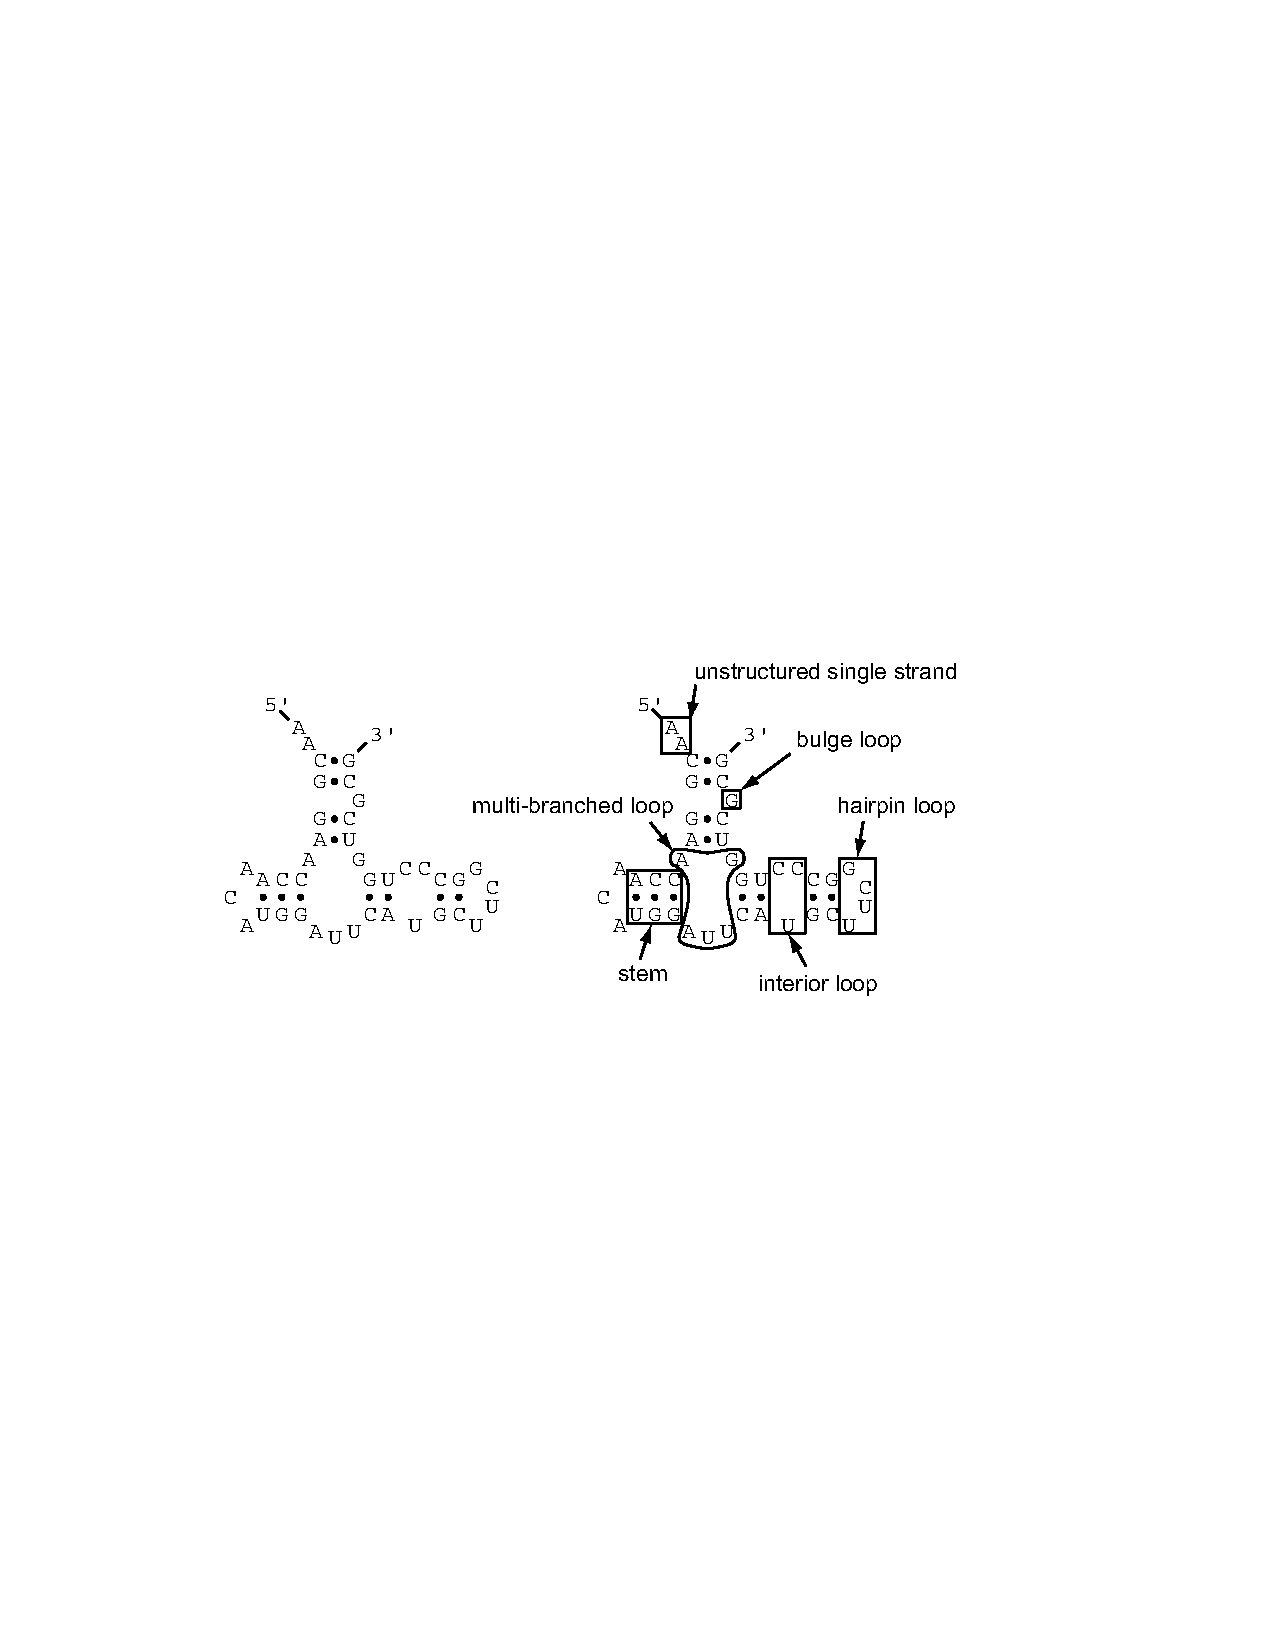
\includegraphics[scale=0.8]{Figures/rna_elements}
\end{center}
\begin{center}
\begin{BVerbatim}
  ::((((,<<<___>>>,,,<<-<<____>>-->>,))-))
  AACGGAACCAACAUGGAUUCAUGCUUCGGCCCUGGUCGCG
\end{BVerbatim}
\end{center}

\subsubsection{Full (output) WUSS notation}

In detail, symbols used by WUSS notation in \emph{output} structure
annotation strings are as follows:

\begin{sreitems}{\textbf{Bulge, interior loops}}
\item[\textbf{Base pairs}]
  Base pairs are annotated by nested matching pairs of symbols
  \verb+<>+, \verb+()+, \verb+[]+, or \verb+{}+.
  The different symbols indicate the ``depth'' of the
  helix in the RNA structure as follows:
  \verb+<>+ are used for simple terminal stems; 
  \verb+()+ are used for ``internal'' helices enclosing a multifurcation of
  all terminal stems; \verb+[]+ are used for internal helices 
  enclosing a multifurcation that includes at least one annotated
  \verb+()+ stem already; and \verb+{}+ are used for all internal
  helices enclosing deeper multifurcations.
   
\item[\textbf{Hairpin loops}]
  Hairpin loop residues are indicated by underscores, \verb+_+.
  Simple stem loops stand out as, e.g.\ \verb+<<<<____>>>>+.

\item[\textbf{Bulge, interior loops}]
  Bulge and interior loop residues are indicated by dashes, \verb+-+.
  
\item[\textbf{Multifurcation loops}]
  Multifurcation loop residues are indicated by commas, \verb+,+.
  The mnemonic is ``stem 1, stem2'', e.g.\ \verb+<<<___>>>,,<<<___>>>+.

\item[\textbf{External residues}]
  Unstructured single stranded residues completely outside the
  structure (unenclosed by any base pairs) are annotated by
  colons, \verb+:+.

\item[\textbf{Insertions}]
  Insertions relative to a known structure are indicated by periods,
  \verb+.+. Regions where local structural alignment was invoked,
  leaving regions of both target and query sequence unaligned,
  are indicated by tildes, \verb+~+. These symbols only appear in
  alignments of a known (query) structure annotation to a target
  sequence of unknown structure.

\item[\textbf{Pseudoknots}]
  WUSS notation allows pseudoknots to be annotated as pairs of
  upper case/lower case letters: for example,
  \verb+<<<<_AAAA____>>>>aaaa+ annotates a simple pseudoknot;
  additional pseudoknotted stems could be annotated by \verb+Bb+,
  \verb+Cc+, etc. Infernal cannot handle pseudoknots, however;
  pseudoknot notation never appears in Infernal output; it
  is accepted in input files, but ignored.
\end{sreitems}

An example of WUSS notation for a complicated structure
(\emph{E. coli} RNase P) is shown in Figure~\ref{fig:RNaseP}.  An
example of WUSS notation for a local Infernal alignment of
\emph{B. subtilis} RNase P to \emph{E. coli} RNase P, illustrating the
use of local alignment annotation symbols, is in
Figure~\ref{fig:bsu-alignment}.

\begin{figure}[tp]
\begin{center}
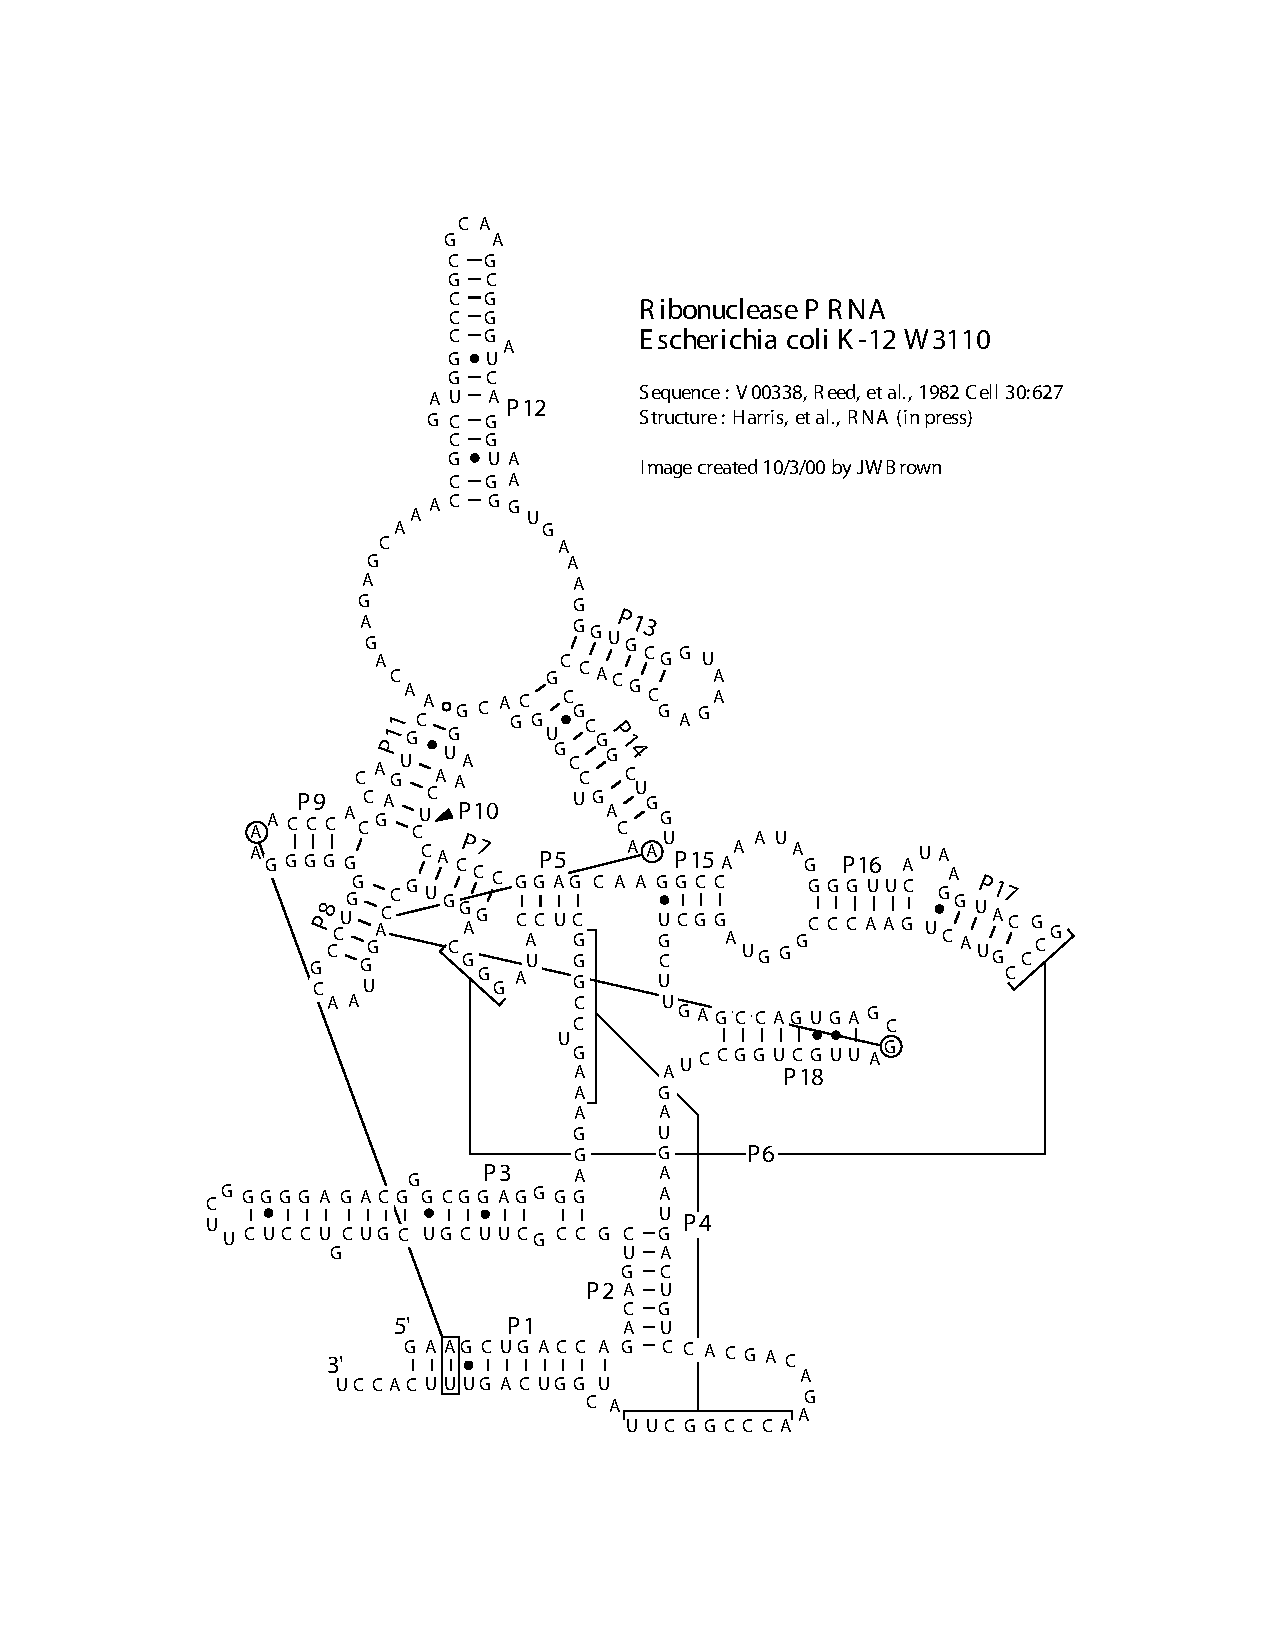
\includegraphics[scale=0.6]{Figures/rnaseP-ecoli}
\end{center}        
\begin{center}
{\scriptsize
\begin{BVerbatim}
           {{{{{{{{{{{{{{{{{{,<<<<<<<<<<<<<-<<<<<____>>>>>>>>>->>>>>>>>
         1 GAAGCUGACCAGACAGUCGCCGCUUCGUCGUCGUCCUCUUCGGGGGAGACGGGCGGAGGG 60      

           >,,,,,,,,,,,,,[[[[--------[[[[[<<<<<_____>>>>><<<<____>>>->(
        61 GAGGAAAGUCCGGGCUCCAUAGGGCAGGGUGCCAGGUAACGCCUGGGGGGGAAACCCACG 120     

           (---(((((,,,,,,,,,,,,<<<<<--<<<<<<<<____>>>>>->>>>>>-->>,,,,
       121 ACCAGUGCAACAGAGAGCAAACCGCCGAUGGCCCGCGCAAGCGGGAUCAGGUAAGGGUGA 180     

           ,,,<<<<<<_______>>>>>><<<<<<<<<____>>>->>>>>->,,)))--))))]]]
       181 AAGGGUGCGGUAAGAGCGCACCGCGCGGCUGGUAACAGUCCGUGGCACGGUAAACUCCAC 240     

           ]]]]]],,,<<<<------<<<<<<----<<<<<_____>>>>>>>>>>>----->>>>,
       241 CCGGAGCAAGGCCAAAUAGGGGUUCAUAAGGUACGGCCCGUACUGAACCCGGGUAGGCUG 300     

           ,,,,,<<<<<<<<____>>>>>>>>,,,,,,,,,,}}}}}}}------------------
       301 CUUGAGCCAGUGAGCGAUUGCUGGCCUAGAUGAAUGACUGUCCACGACAGAACCCGGCUU 360     

           -}-}}}}}}}}}}::::
       361 AUCGGUCAGUUUCACCU 377     
\end{BVerbatim} 
}
\end{center}
\caption{\small \textbf{Example of WUSS notation.} Top: Secondary
structure of \emph{E. coli} RNase P, from Jim Brown's RNase P database
\citep{Brown99}. Bottom: WUSS notation for the same structure,
annotating the \emph{E. coli} RNase P sequence. The P4 and P6
pseudoknots are not annotated in this example.}
\label{fig:RNaseP}
\end{figure}

\begin{figure}[tp]
\begin{center}
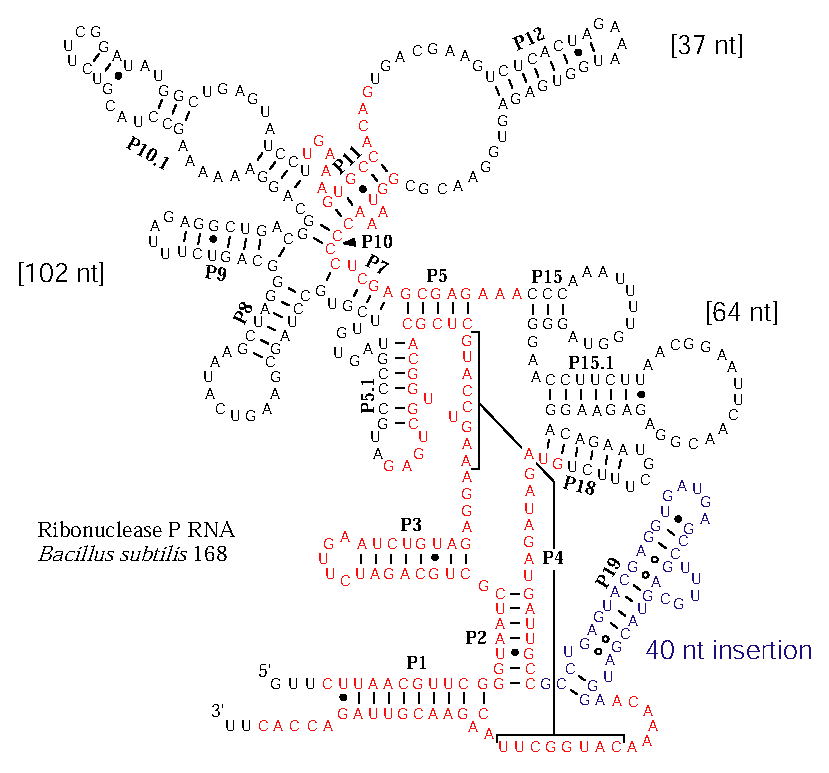
\includegraphics[scale=0.6]{Figures/rnaseP-bsu-alignment}
\end{center}
\begin{center}
{\scriptsize
\begin{BVerbatim}
>> M13175.1  
 rank     E-value  score  bias mdl mdl from   mdl to       seq from      seq to       acc trunc   gc
 ----   --------- ------ ----- --- -------- --------    ----------- -----------      ---- ----- ----
  (1) !   2.2e-20   58.0   0.0  cm        1      367 []           4         399 + .. 0.77    no 0.49

                    v                          v      v                                  vv         vvvvv    vvvv vv NC
                    {{{{{{{{{{{{{{{{{{,<<<<<<<<<______>>>>>>>>>,,,,,,,,,,,,,[[[[.--------[[[[[~~~~~~<<<<<____>>>>->( CS
  RNaseP_bact_a   1 cgagccggccgggcggucGCgcccccccuuaaaagggggggcGAGGAAAGUCCGGgCUcC.AcAGGgCAggguG*[15]*cggggGugAccccAgG 104
                       ::CG::CGGG:::UCGC::C:::: U      ::::G::GAGGAAAGUCC  GCUC  AC G GC   G:G               +++C + 
       M13175.1   4 CUUAACGUUCGGGUAAUCGCUGCAGAUCU---UGAAUCUGUAGAGGAAAGUCCAUGCUCGcACGGUGCU--GAG*[96]*---------UAUCCUU 175
                    **************************974...4579**********************98788777776..555...8...........3444468 PP

                                                                                           v   vv        vvvv        NC
                    (---(((((,,,,,,,,,,,,<<<<<<<<<<<____>>>>>>>>>-->>,,,,,,~~~~~~,,)))--))))]]]]].]]]],,,<<<<-----   CS
  RNaseP_bact_a 105 GAaAGugCcACAGAAAaaAgACCgCccgccccuuaaggggcggGcAAGGGUGAAA*[43]*uagGcAAaCCCCaccc.GgAGCAAggccAAAUA   234
                    GAAAGU:CCACAG +A  A+ :C   :::C:: +AA::G:::     G:GUG AA        GG:AAACC C:C +  GAG AA  C+AA U 
       M13175.1 176 GAAAGUGCCACAGUGACGAAGUC---UCACUAGAAAUGGUGA-----GAGUGGAA*[ 1]*GCGGUAAACCCCUCGAgCGAGAAACCCAAAUUU   256
                    99*****************8866...4455558888555444.....66999987...6..99********97665577899888765444332   PP

                          vvvv                                                                                       NC
                    ~~~~~~>>>>,,,,,,<<<<<<.<<____>>>>>>>>,,,,,,,,,,}}}}}}}---------------........................--- CS
  RNaseP_bact_a 235 *[39]*ggccGCUuGAGccggc.cgGuAAcggccggCCuAGAugAAUgaccgcccucuuguuaaauuuu........................aAC 338
                              G     :::: : C:G AA:G: :::: UAGAU++AUGA:::CC  CU + UA  +  U                        AAC
       M13175.1 257 *[32]*----GAG---AGAAGGaCAG-AAUGCUUUCUGUAGAUAGAUGAUUGCCGCCUGAGUACGAGGUgaugagccguuugcaguacgauggAAC 370
                    ...3......222...2222221222.335555566699****************9998888888888899999********************** PP

                                            v     NC
                    -------------}-}}}}}}}}}}:::: CS
  RNaseP_bact_a 339 AGAAcCCGGCUUAcaggccggcucgucuu 367
                    A AAC  GGCUUACAG::CG::    C+ 
       M13175.1 371 AAAACAUGGCUUACAGAACGUUAGACCAC 399
                    ***************************** PP
\end{BVerbatim}
}
\end{center}
\caption{\small \textbf{Local alignment annotation example.} Top:
Secondary structure of \emph{B. subtilis} RNase P, from Jim Brown's
RNase P database \citep{Brown99}. Residues in red are those that
Infernal aligns to a CM of \emph{E. coli} type RNase P's
(the RNase P bacterial type A model built from the Rfam 10.1 RF00010
seed alignment using default Infernal 1.1 \prog{cmbuild} and
\prog{cmcalibrate}). The local structural alignment is in four pieces;
three regions of the structure (96, 1, and 32 nt long) are skipped
over (i.e. not aligned to the type A model). One additional stem is
treated as a 24 nt insertion.  Bottom: the Infernal \prog{cmsearch}
output showing the RNase P type A query model, which corresponds
closely to the \emph{E. coli} structure, aligned to the
\emph{B. subtilis} sequence. The three skipped regions (96, 1, and 32
nt long) of the \emph{B. subtilis} structure from the top of the
figure are ``local end'' emissions which skip 15, 43, and 39 consensus
positions of the type A model, respectively.}
\label{fig:bsu-alignment}
\end{figure}

\subsubsection{Shorthand (input) WUSS notation}

While WUSS notation makes it easier to visually interpret
Infernal \emph{output} structural annotation, it would be
painful to be required to \emph{input} all structures in full WUSS
notation. Therefore when Infernal reads input secondary
structure annotation, it uses simpler rules:

\begin{sreitems}{\textbf{Single stranded residues}}
\item [\textbf{Base pairs}]
  Any matching nested pair of \verb+()+, \verb+()+, \verb+[]+, \verb+{}+
  symbols indicates a base pair; the exact choice of symbol has no
  meaning, so long as the left and right partners match up.

\item [\textbf{Single stranded residues}]
  All other symbols \verb+_-,:.~+ 
  indicate single stranded residues.
  The choice of symbol has no special meaning.
  Annotated pseudoknots (nested matched pairs of upper/lower case
  alphabetic characters) are also interpreted as single
  stranded residue in Infernal input.
\end{sreitems}

Thus, for instance, \verb+<<<<....>>>>+ and \verb+((((____))))+ and
\verb+<(<(._._)>)>+ all indicate a four base stem with a four base
loop (the last example is legal but weird). 

Remember that the key property of canonical (nonpseudoknotted) RNA
secondary structure is that the pairs are \emph{nested}.
\verb+((<<....))>>+ is not a legal annotation string: the pair symbols
don't match up properly. Infernal will reject such an
annotation and report an input format error, suspecting a problem with
your annotation.  If you want to annotate pseudoknots, WUSS notation
allows alphabetic symbols Aa, Bb, etc.\, see above; but remember that
Infernal ignores pseudoknotted stems and treats them as
single stranded residues.

Because many other RNA secondary structure analysis programs use a
simple bracket notation for annotating structure,
Infernal's ability to input this format makes it easier to
use data generated by other RNA software packages. Conversely,
converting Infernal output WUSS notation to simple bracket
notation is a matter of a simple Perl or sed script, substituting the
symbols appropriately.

\subsection{Stockholm, the recommended multiple sequence alignment format}

The Rfam and Pfam Consortiums have developed a multiple sequence
alignment format called ``Stockholm format'' that allows rich and
extensible annotation. 

Crucially for Infernal, Stockholm alignments support the annotation of 
a consensus secondary structure, which is why \prog{cmbuild} requires
its input alignment files to be in Stockholm format. Here is a minimal
Stockholm file with consensus secondary structure annotation in
shorthand WUSS notation (described earlier in this section).

\begin{sreoutput}
# STOCKHOLM 1.0

seq1           ACCGUC...GCAA...GG
seq2           ACCGUC...GCAA...GG
seq3           .CCUUCGUCGGAUGACGA
#=GC SS_cons   ...<<<..........>>

seq1           CGAUAC
seq2           CG..AC
seq3           ACAUCC
#=GC SS_cons   >.....
//
\end{sreoutput}

The first line in the file must be \verb+# STOCKHOLM 1.x+, where
\verb+x+ is a minor version number for the format specification
(and which currently has no effect on my parsers). This line allows a
parser to instantly identify the file format.

In the alignment, each line contains a name, followed by the aligned
sequence. A dash, period, underscore, or tilde (but not whitespace)
denotes a gap. If the alignment is too long to fit on one line, the
alignment may be split into multiple blocks, with blocks separated by
blank lines, as this example is. The number of sequences, their order,
and their names must be the same in every block. Within a given block,
each (sub)sequence (and any associated \verb+#=GR+ and \verb+#=GC+
markup, such as the \verb+SS_cons+ lines, see below) is of equal
length, called the \textit{block length}. Block lengths may differ
from block to block. The block length must be at least one residue,
and there is no maximum. 

Other blank lines are ignored. You can add comments anywhere to the
file (even within a block) on lines starting with a \verb+#+.

The \verb+SS_cons+ line defines the consensus secondary structure in
shorthand WUSS notation, as described earlier in 
this section.

All other annotation is added using a tag/value comment style. The
tag/value format is inherently extensible, and readily made
backwards-compatible; unrecognized tags will simply be ignored. Extra
annotation includes individual sequence RNA or protein secondary
structure, sequence weights, a reference coordinate system for the
columns, and database source information including name, accession
number, and coordinates (for subsequences extracted from a longer
source sequence) See below for details.

\subsubsection{syntax of Stockholm markup}

There are four types of Stockholm markup annotation, for per-file,
per-sequence, per-column, and per-residue annotation:

\begin{sreitems}{\emprog{\#=GR <seqname> <tag> <..s..>}}
\item [\emprog{\#=GF <tag> <s>}]
        Per-file annotation. \prog{<s>} is a free format text line
        of annotation type \prog{<tag>}. For example, \prog{\#=GF DATE
        April 1, 2000}. Can occur anywhere in the file, but usually
        all the \prog{\#=GF} markups occur in a header.

\item [\emprog{\#=GS <seqname> <tag> <s>}]
        Per-sequence annotation. \prog{<s>} is a free format text line
        of annotation type \prog{tag} associated with the sequence
        named \prog{<seqname>}. For example, \prog{\#=GS seq1
        SPECIES\_SOURCE Caenorhabditis elegans}. Can occur anywhere
        in the file, but in single-block formats (e.g. the Pfam
        distribution) will typically follow on the line after the
        sequence itself, and in multi-block formats (e.g. Infernal
        output), will typically occur in the header preceding the
        alignment but following the \prog{\#=GF} annotation.

\item [\emprog{\#=GC <tag> <..s..>}]
        Per-column annotation. \prog{<..s..>} is an aligned text line
        of annotation type \prog{<tag>}.
        \verb+#=GC+ lines are
        associated with a sequence alignment block; \prog{<..s..>}
        is aligned to the residues in the alignment block, and has
        the same length as the rest of the block.
        Typically \verb+#=GC+ lines are placed at the end of each block.

\item [\emprog{\#=GR <seqname> <tag> <..s..>}]
        Per-residue annotation. \prog{<..s..>} is an aligned text line
        of annotation type \prog{<tag>}, associated with the sequence
        named \prog{<seqname>}. 
        \verb+#=GR+ lines are 
        associated with one sequence in a sequence alignment block; 
        \prog{<..s..>}
        is aligned to the residues in that sequence, and has
        the same length as the rest of the block.
        Typically
        \verb+#=GR+ lines are placed immediately following the
        aligned sequence they annotate.
\end{sreitems}

\subsubsection{semantics of Stockholm markup}

Any Stockholm parser will accept syntactically correct files, but is
not obligated to do anything with the markup lines. It is up to the
application whether it will attempt to interpret the meaning (the
semantics) of the markup in a useful way. At the two extremes are the
Belvu alignment viewer and the Infernal and HMMER 
software packages.

Belvu simply reads Stockholm markup and displays it, without trying to
interpret it at all. The tag types (\prog{\#=GF}, etc.) are sufficient
to tell Belvu how to display the markup: whether it is attached to the
whole file, sequences, columns, or residues.

Infernal uses Stockholm markup to pick up a variety of information
from the Rfam multiple alignment database. The Rfam consortium
therefore agrees on additional syntax for certain tag types, so
Infernal can parse some markups for useful information. This
additional syntax is imposed by Rfam, Pfam, Infernal, HMMER, and other
software from our lab, not by Stockholm format per se. You can think
of Stockholm as akin to XML, and what our software reads as akin
to an XML DTD, if you're into that sort of structured data format
lingo.

The Stockholm markup tags that are parsed semantically by Infernal
are as follows:

\subsubsection{recognized \#=GF annotations}
\begin{sreitems}{\emprog{TC  <f> <f>}}
\item [\emprog{ID  <s>}] 
        Identifier. \emprog{<s>} is a name for the alignment;
        e.g. ``RNaseP''. One word. Unique in file.

\item [\emprog{AC  <s>}]
        Accession. \emprog{<s>} is a unique accession number for the
        alignment; e.g. 
        ``RF00001''. Used by the Rfam database, for instance. 
        Often a alphabetical prefix indicating the database
        (e.g. ``RF'') followed by a unique numerical accession.
        One word. Unique in file. 
        
\item [\emprog{DE  <s>}]
        Description. \emprog{<s>} is a free format line giving
        a description of the alignment; e.g.
        ``Ribonuclease P RNA''. One line. Unique in file.

\item [\emprog{AU  <s>}]
        Author. \emprog{<s>} is a free format line listing the 
        authors responsible for an alignment; e.g. 
        ``Bateman A''. One line. Unique in file.

\item [\emprog{GA  <f>}]
        Gathering threshold. The Infernal bit score cutoff 
        used in gathering the members of Rfam full alignments. 
        
\item [\emprog{NC <f>}] 
        Noise cutoff. The Infernal bit score cutoff, set according to
        the highest scores seen for nonhomologous sequence hits when
        gathering members of Rfam full alignments.

\item [\emprog{TC  <f>}]
        Trusted cutoff. The Infernal bit score cutoff, set according
        to the lowest scores seen for true homologous sequence hits
        that were above the GA gathering thresholds, when gathering
        members of Rfam full alignments.
\end{sreitems}

\subsubsection{recognized \#=GS annotations}

\begin{sreitems}{\emprog{WT  <f>}}
\item [\emprog{WT  <f>}]
        Weight. \emprog{<f>} is a positive real number giving the
        relative weight for a sequence, usually used to compensate
        for biased representation by downweighting similar sequences.   
        Usually the weights average 1.0 (e.g. the weights sum to
        the number of sequences in the alignment) but this is not
        required. Either every sequence must have a weight annotated, 
        or none of them can.  

\item [\emprog{AC  <s>}]
        Accession. \emprog{<s>} is a database accession number for 
        this sequence. (Compare the \prog{\#=GF AC} markup, which gives
        an accession for the whole alignment.) One word. 
        
\item [\emprog{DE  <s>}]
        Description. \emprog{<s>} is one line giving a description for
        this sequence. (Compare the \prog{\#=GF DE} markup, which gives
        a description for the whole alignment.)
\end{sreitems}


\subsubsection{recognized \#=GC annotations}

\begin{sreitems}{\emprog{SS\_cons}}
\item [\emprog{RF}]
        Reference line. Any character is accepted as a markup for a
        column. The intent is to allow labeling the columns with some
        sort of mark. \prog{cmbuild} uses this annotation to determine
        which columns are consensus versus insertion if the
        \prog{--hand} option is used; insertion columns are annotated
        by a gap symbol, and consensus columns by any non-gap symbol.
        
\item [\emprog{SS\_cons}]
	Secondary structure consensus.  When this line is generated by
        Infernal, it is generated in full WUSS notation.
        When it is read by \prog{cmbuild}, it is interpreted more
        loosely, in shorthand (input) WUSS notation: pairs of symbols
        \verb+<>+, \verb+()+, \verb+[]+, or \verb+[]+ mark consensus
        base pairs, and symbols \verb+:_-,.~+ mark single stranded
        columns (see the section on WUSS format above for details).

\end{sreitems}

\subsubsection{recognized \#=GR annotations}
\begin{sreitems}{\emprog{SS}}
\item [\emprog{SS}]
        Secondary structure consensus. See \prog{\#=GC SS\_cons}
        above.

\item [\emprog{PP}] Posterior probability for an aligned residue. This
  represents the probability that this residue is assigned to the CM
  state corresponding to this alignment column, as opposed to some
  other state. The posterior
  probability is encoded as 11 possible characters \verb+0-9*+: $0.0
  \leq p < 0.05$ is coded as 0, $0.05 \leq p < 0.15$ is coded as 1,
  (... and so on ...), $0.85 \leq p < 0.95$ is coded as 9, and $0.95
  \leq p \leq 1.0$ is coded as '*'. Gap characters appear in the PP
  line where no residue has been assigned.
\end{sreitems}

\subsection{Sequence files: FASTA format}

FASTA is probably the simplest of formats for unaligned sequences.
FASTA files are easily created in a text editor.  Each sequence is
preceded by a line starting with \verb+>+. The first word on this line
is the name of the sequence. The rest of the line is a description of
the sequence (free format). The remaining lines contain the sequence
itself. You can put as many letters on a sequence line as you want.
For example:

\begin{sreoutput}
>seq1 This is the description of my first sequence.
AGTACGTAGTAGCTGCTGCTACGTGCGCTAGCTAGTACGTCA CGACGTAGATGCTAGCTGACTCGATGC
>seq2 This is a description of my second sequence.
CGATCGATCGTACGTCGACTGATCGTAGCTACGTCGTACGTAG CATCGTCAGTTACTGCATGCTCG
CATCAGGCATGCTGCTGACTGATCGTACG
\end{sreoutput}

For better or worse, FASTA is not a documented standard. Minor (and
major) variants are in widespread use in the bioinformatics community,
all of which are called ``FASTA format''. My software attempts to
cater to all of them, and is tolerant of common deviations in FASTA
format. Certainly anything that is accepted by the database formatting
programs in NCBI BLAST or WU-BLAST (e.g. setdb, pressdb, xdformat)
will also be accepted by my software. Blank lines in a FASTA file are
ignored, and so are spaces or other gap symbols (dashes, underscores,
periods) in a sequence. Other non-amino or non-nucleic acid symbols in
the sequence are also silently ignored, mostly because some people
seem to think that ``*'' or ``.'' should be added to protein sequences
to (redundantly) indicate the end of the sequence. The parser will
also accept unlimited line lengths, which allows it to accomodate the
enormous description lines in the NCBI NR databases.

(On the other hand, any FASTA files \emph{generated} by my software
adhere closely to community standards, and should be usable by other
software packages (BLAST, FASTA, etc.) that are more picky about
parsing their input files. That means you can run a sloppy FASTA file
thru the \prog{sreformat} utility program to clean it up.)

Partly because of this tolerance, the software may have a difficult
time dealing with files that are \textit{not} in FASTA format,
especially if you're relying on file format autodetection (the
``Babelfish'').  Some (now mercifully uncommon) file formats are so
similar to FASTA format that they be erroneously called FASTA by the
Babelfish and then quietly and lethally misparsed. An example is the
old NBRF file format. If you're afraid of this, you can use the
\prog{--informat fasta} option to bypass the Babelfish and improve
robustness. However, it is still possible to construct files
perversely similar to FASTA that will still confuse the parser.  (The
gist of these caveats applies to all formats, not just FASTA.)

\subsection{Null model file format}

The Infernal source distribution includes an example null model file, 
\prog{src/rna.null}. This null model is identical to the hardcoded default
prior used by Infernal, all four RNA nucleotides are equiprobable in
the null, background model. 

A null model file must contain exactly four non-comment lines. A
comment line begins with a ``\# ``, that is a \# followed by a single
space. Each of the four non-comment lines must contain a single floating point
number, the four of which sum to 1.0. The first non-comment line is interpreted as
the background probability of an ``A'' residue, the second, third, and
fourth non-comment lines are interpreted as the background
probabilities of a ``C'', ``G'' and ``U'' respectively. 

\subsection{Clan input file format for cmscan}

The \ccode{cmscan} program has a \ccode{--clanin <f>} option that
allows the user to supply an input file \ccode{<f>} with information
on clan membership for models in the CM file. This option must be used
in combination with the \ccode{--tblout} and \ccode{--fmt 2}
options. An example clan input file is included with the Infernal
source distribution, \ccode{tutorial/Rfam.12.1.clanin}. This file
specifies the clan membership for the 2474 models in the Rfam 12.1
release, of which 311 models belong to 104 clans. This file should be
used in combination with the Rfam.cm file for Rfam 12.1, available for
download as a gzipped file here:
\url{ftp://ftp.ebi.ac.uk/pub/databases/Rfam/12.1/Rfam.cm.gz}. Note that
many of the Rfam models are not members of a clan; the clan input file does
not need to specify clan membership for all models in the CM file.

A clan input file contains one line per clan. Each line must contain
at least two space-delimited tokens. The first token is the name of
the clan (this name cannot contain spaces). Each token after the first
is the name of a model that is a member of the clan named in the first
token. These tokens must be valid names of models in the file CM file
you are using with \ccode{cmscan}. These tokens cannot be the
accessions of models. Valid model names cannot contain spaces
(enforced by \prog{cmbuild} during model construction). To determine
the names of models in a CM file, use \ccode{cmstat}. 

For example, in the file \ccode{tutorial/Rfam.12.1.clanin} the first token
of the first line is ``CL00001'' and tokens two through five are
``tRNA'', ``cyano\_tmRNA'', ``tRNA-Sec'', ``mt-tmRNA'', indicating
that these four models are members of the CL00001 clan. \ccode{cmscan}
will output the clan name of models in clans in its tabular output
file specified with \ccode{--tblout} when the \ccode{--fmt 2} option
is also used. Furthermore, you can specify
that only overlapping hits between models of the same clan are
annotated (as opposed to all overlapping hits) in the tabular output
file by additionally using the \ccode{--oclan} option. Finally, you
can specify that lower scoring overlaps within clans are not output by
additionally using the \ccode{--oskip} and the \ccode{--oclan}
options.





\subsection{Dirichlet prior files}
% Documentation of Infernal's Dirichlet prior file format
%
% Uses no sectioning commands, so it may be included as a subsection of
% a section, or a section in a chapter of file formats.
% The .tex file that includes this one provides the \section{} header.
%  
% SRE, Wed Apr  6 13:46:43 2005
% SVN $Id$

A prior file is parsed into a number of whitespace-delimited,
non-comment fields. These fields are then interpreted in order.  The
order and number of the fields is important. This is not a robust,
tag-value save file format.

All whitespace is ignored, including newlines. The number of fields
per line is unimportant.

Comments begin with a \verb+#+ character. The remainder of any line
following a \verb+#+ is ignored.

The Infernal source distribution includes an example prior file,
\prog{default.pri}. This prior is identical to the hardcoded default
prior used by Infernal. The following text may only make sense if
you're looking at that example while you read.

The order of the fields in the prior file is as follows:

\begin{description}
\item[\textbf{Strategy.}] The first field is the keyword
  \emprog{Dirichlet}. Currently Dirichlet priors (mixture or not)
  are the only prior strategy used by Infernal.

\item[\textbf{Transition prior section.}] The next field is the number
  \emprog{74}, the number of different types of transition
  distributions. (See Figure~\ref{fig:magic74} for an explanation of
  where the number 74 comes from.) Then, for each of these 74
  distributions:

  \begin{description}
  \item{\emprog{<from-uniqstate> <to-node>}:} Two fields give the
  transition type: from a unique state identifier, to a node
  identifier. Example: \emprog{MATP\_MP MATP}. 

  \item{\emprog{<n>}:} One field gives the number of transition
  probabilities for this transition type; that is, the number of
  Dirichlet parameter vector $\alpha^q_1..\alpha^q_n$ for each mixture
  component $q$.

  \item{\emprog{<nq>}:} One field gives the number of mixture
  Dirichlet components for this transition type's prior. Then,
  for each of these \emprog{nq} Dirichlet components:

     \begin{description}
     \item{\emprog{p(q)}:} One field gives the mixture coefficient $p(q)$,
     the prior probability of this component $q$. For a single-component
     ``mixture'', this is always 1.0.

     \item{$\mathbf{\alpha^q_1..\alpha^q_n}$:} The next $n$ fields give the
     Dirichlet parameter vector for this mixture component $q$.
     \end{description}
  \end{description}

\item[\textbf{Base pair emission prior section.}] This next section is
  the prior for MATP\_MP emissions. One field gives \emprog{<K>}, the
  ``alphabet size'' -- the number of base pair emission probabilities
  -- which is always 16 (4x4), for RNA. The next field gives \emprog{<nq>}, the
  number of mixture components. Then, for each of these \emprog{nq}
  Dirichlet components:
     \begin{description}
     \item{\emprog{p(q)}:} One field gives the mixture coefficient $p(q)$,
     the prior probability of this component $q$. For a single-component
     ``mixture'', this is always 1.0.

     \item{$\mathbf{\alpha^q_{AA}..\alpha^q_{UU}}$:} The next 16 fields give the
     Dirichlet parameter vector for this mixture component, in alphabetical
     order (AA, AC, AG, AU, CA \ldots GU, UA, UC, UG, UU). 
     \end{description}

\item[\textbf{Consensus singlet base emission prior section.}] This
  next section is the prior for MATL\_ML and MATR\_MR emissions.  One
  field gives \emprog{<K>}, the ``alphabet size'' -- the number of
  singlet emission probabilities -- which is always 4, for RNA.  The
  next field gives \emprog{<nq>}, the number of mixture components. Then,
  for each of these \emprog{nq} Dirichlet components:
     \begin{description}
     \item{\emprog{p(q)}:} One field gives the mixture coefficient $p(q)$,
     the prior probability of this component $q$. For a single-component
     ``mixture'', this is always 1.0.

     \item{$\mathbf{\alpha^q_A..\alpha^q_U}$:} The next 4 fields give the
     Dirichlet parameter vector for this mixture component, in alphabetical
     order (A, C, G, U).
     \end{description}
  
\item[\textbf{Nonconsensus singlet base emission prior section.}] This
  next section is the prior for insertions (MATP\_IL, MATP\_IR,
  MATL\_IL, MATR\_IR, ROOT\_IL, ROOT\_IR, BEGR\_IL) as well as
  nonconsensus singlets (MATP\_ML, MATP\_MR). 
  One field gives \emprog{<K>}, the ``alphabet size'' -- the number of
  singlet emission probabilities -- which is always 4, for RNA. 
  The next field gives \emprog{<nq>}, the
  number of mixture components. Then, for each of these \emprog{nq}
  Dirichlet components:
     \begin{description}
     \item{\emprog{p(q)}:} One field gives the mixture coefficient $p(q)$,
     the prior probability of this component $q$. For a single-component
     ``mixture'', this is always 1.0.

     \item{$\mathbf{\alpha^q_A..\alpha^q_U}$:} The next 4 fields give the
     Dirichlet parameter vector for this mixture component, in alphabetical
     order (A, C, G, U).
     \end{description}
\end{description}


\begin{figure}[htp]
\begin{center}
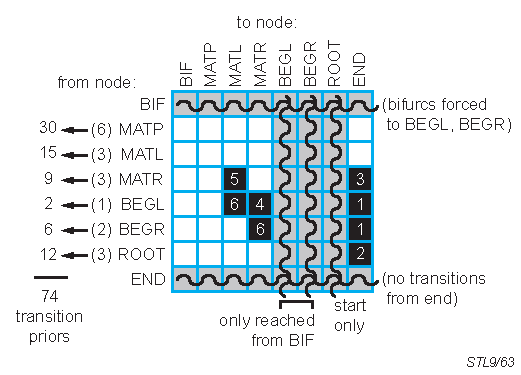
\includegraphics{Figures/stl9-63}
\end{center}
\caption{\small\textbf{Where does the magic number of 74 transition
distribution types come from?} The transition distributions are
indexed in a 2D array, from a unique statetype (20 possible) to a
downstream node (8 possible), so the total conceivable number of
different distributions is $20 \times 8 = 160$. The grid represents
these possibilities by showing the $8 \times 8$ array of all node
types to all node types; each starting node contains 1 or more unique
states (number in parentheses to the left).
Two rows are impossible (gray): bifurcations automatically transit to
determined BEGL, BEGR states with probability 1, and end nodes have no
transitions.  Three columns are impossible (gray): BEGL and BEGR can
only be reached by probability 1 transitions from a bifurcation, and
the ROOT node is special and can only start a model. 
Eight individual cells of the grid are unused (black) because of the
way \prog{cmbuild} (almost) unambiguously constructs a guide tree from
a consensus structure.  These cases are numbered as follows. (1) BEGL
and BEGR never transit to END; this would imply an empty
substructure. A bifurcation is only used if both sides of the split
contain at least one consensus pair (MATP). (2) ROOT never transits to
END; this would imply an alignment with zero consensus
columns. Infernal models assume $\geq 1$ consensus columns. (3) MATR
never transits to END. Infernal always uses MATL for unpaired columns
whenever possible. MATR is only used for internal loops,
multifurcation loops, and 3' bulges, so MATR must always be followed
by a BIF, MATP, or another MATR. (4) BEGL never transits to MATR. The
single stranded region between two bifurcated stems is unambiguously
assigned to MATL nodes on the right side of the split, not to MATR
nodes on the left. (5) MATR never transits to MATL. The only place
where this could arise (given that we already specified that MATL is
used whenever possible) is in an interior loop; there, by unambiguous
convention, MATL nodes precede MATR nodes. (6) BEGL nodes never
transit to MATL, and BEGR nodes never transit to MATR. By convention,
at any bifurcated subsequence $i,j$, $i$ and $j$ are paired but not to
each other. That is, the smallest possible subsequence is bifurcated,
so that any single stranded stretches to the left and right are
assigned to MATL and MATR nodes above the bifurcation, instead of MATL
nodes below the BEGL and MATR nodes below the BEGR.
Thus, the total number 74 comes from multiplying, for each row, the
number of unique states in each starting node by the number of
possible downstream nodes (white), and summing these up, as shown to
the left of the grid.}
\label{fig:magic74}
\end{figure}

\newpage
\section{Acknowledgements}

Infernal relies heavily on HMMER and Easel, originally created by Sean
Eddy. Several others have helped develop these two packages as well,
including Steve Johnson, Alex Coventry, Dawn Brooks, Sergi Castellano,
Michael Farrar, Travis Wheeler, and Elena Rivas.  In particular, the
improved speed of Infernal 1.1 is enabled by research and development
for the HMMER3 project, mainly from Sean, Travis and Michael. Further,
many of the changes made for Infernal 1.1 mirror features in HMMER3,
and were implemented frequently by stealing and slightly modifying
code. Even this guide is based heavily on HMMER3's guide, and some
analogous sections are identical or near identical.  Additionally, the
RSEARCH program \citep{KleinEddy03} from Robbie Klein has also had an
important impact on Infernal, which still includes some of its code.

Sean created and was the lone developer of Infernal up through the
version 0.55 release in 2003. Two graduate students, Diana Kolbe and
Eric Nawrocki, focused on improvements to Infernal for their graduate
work, beginning in 2004. Their efforts combined with Sean's led to
versions 0.56 through 1.0.2. Diana has moved onto a postdoc, but
included a snapshot of the codebase in between the 1.0.2 and 1.1
releases as supplementary material with her thesis. Eric continues to
develop Infernal and is responsible for most of the changes in the 1.1
release.

The concept of HMM banded SCFG alignment implemented in Infernal
derives from Michael Brown's RNACAD software, developed while he was
working with David Haussler at UC Santa Cruz \citep{Brown00}. HMM
filtering for CMs was pioneered by Zasha Weinberg and Larry Ruzzo at
the University of Washington
\citep{WeinbergRuzzo04,WeinbergRuzzo04b,WeinbergRuzzo06}. The CP9 HMMs
in Infernal are a reimplementation of a profile HMM architecture
introduced by Weinberg.

Infernal testing requires \emph{a lot} of compute power, and we are
extremely fortunate to have access to a highly reliable and
state-of-the-art computing cluster, thanks to Jesse Becker, Ron
Patterson and others at NCBI.

Infernal is primarily developed on GNU/Linux and Apple Macintosh
machines, but is tested on a variety of hardware. Over the years,
Compaq, IBM, Intel, Sun Microsystems, Silicon Graphics,
Hewlett-Packard, Paracel, and nVidia have provided generous hardware
support that makes this possible. We owe a large debt to the free
software community for the development tools we use: an incomplete
list includes GNU gcc, gdb, emacs, and autoconf; the amazing valgrind;
the indispensable Subversion; the ineffable perl; LaTeX and TeX;
PolyglotMan; and the UNIX and Linux operating systems.

\label{manualend}


\newpage
\bibliography{master,lab,books,local}
\end{document}
